\documentclass[a4paper]{report}

%====================== PACKAGES ======================

\usepackage[french]{babel}
\usepackage[utf8x]{inputenc}
%pour gérer les positionnement d'images
\usepackage{float}
\usepackage{amsmath}
\usepackage{graphicx}
\usepackage[colorinlistoftodos]{todonotes}
\usepackage{url}
%pour les informations sur un document compilé en PDF et les liens externes / internes
\usepackage{hyperref}
%pour la mise en page des tableaux
\usepackage{array}
\usepackage{tabularx}
%pour utiliser \floatbarrier
%\usepackage{placeins}
%\usepackage{floatrow}
%espacement entre les lignes
\usepackage{setspace}
%modifier la mise en page de l'abstract
\usepackage{abstract}
%police et mise en page (marges) du document
\usepackage[T1]{fontenc}
\usepackage[top=2cm, bottom=2cm, left=2cm, right=2cm]{geometry}
%Pour les galerie d'images
\usepackage{subfig}
\usepackage[dvipsnames]{xcolor}

%====================== INFORMATION ET REGLES ======================

%rajouter les numérotation pour les \paragraphe et \subparagraphe
\setcounter{secnumdepth}{4}
\setcounter{tocdepth}{4}

\hypersetup{							% Information sur le document
pdfauthor = {Premier Auteur,
			Deuxième Auteur,
			Troisième Auteur,
    		Quatrième Auteur},			% Auteurs
pdftitle = {Nom du Projet -
			Sujet du Projet},			% Titre du document
pdfsubject = {Mémoire de Projet},		% Sujet
pdfkeywords = {Tag1, Tag2, Tag3, ...},	% Mots-clefs
pdfstartview={FitH}}					% ajuste la page à la largueur de l'écran
%pdfcreator = {MikTeX},% Logiciel qui a crée le document
%pdfproducer = {}} % Société avec produit le logiciel

%======================== DEBUT DU DOCUMENT ========================

\begin{document}

%régler l'espacement entre les lignes
\newcommand{\HRule}{\rule{\linewidth}{0.5mm}}

%page de garde
\begin{titlepage}
\begin{center}

% Upper part of the page. The '~' is needed because only works if a paragraph has started.

\includegraphics[width=0.35\textwidth]{images/UL.jpg}~\\[1cm]

\textsc{\LARGE Université Catholique de Louvain}\\[1.5cm]

\textsc{\Large }\\[0.5cm]

% Title
\HRule \\[0.4cm]

{\huge \bfseries LSTAT2330 - Synthèse:\\
Statistique des essais cliniques \\[0.4cm] }

\HRule \\[1.5cm]

% Author and supervisor
\begin{minipage}{0.4\textwidth}
\begin{flushleft} \large
\emph{Auteur :}\\
Deside \textsc{Guillaume}\\

\end{flushleft}
\end{minipage}
\begin{minipage}{0.4\textwidth}
\begin{flushright} \large
\emph{Prof :} \\
Catherine \textsc{Legrand}\\
\end{flushright}
\end{minipage}

\vfill

% Bottom of the page
{\large \today}

\end{center}
\end{titlepage}

%page blanche
\thispagestyle{empty}
\newpage
~
\thispagestyle{empty}
\tableofcontents
\thispagestyle{empty}
\setcounter{page}{0}
%ne pas numéroter le sommaire

%\newpage

%espacement entre les lignes d'un tableau
\renewcommand{\arraystretch}{1.5}

%====================== INCLUSION DES PARTIES ======================

~
%\thispagestyle{empty}
%recommencer la numérotation des pages à "1"
\setcounter{page}{0}
%\newpage

\chapter{Prérequis}

\section{Principe des tests d’hypothèse}
On  étudie  une  population  dont  les  éléments  possèdent  un  caractère  (mesurable  ou qualitatif) et dont la valeur du paramètre relative au caractère étudié est inconnue. Une  hypothèse  est  formulée  sur  la  valeur  du  paramètre  :  cette  formulation  résulte  de considérations  théoriques,  pratiques  ou  encore  elle  est  simplement  basée  sur  un pressentiment. Pour  décider  si  l’hypothèse  formulée  est  supportée  ou  non  par  les observations,  il  faut  une  méthode  qui  permettra  de  conclure  si  l’écart  observé  entre  la valeur  de  la  statistique  obtenue  dans  l’échantillon  et  celle  du  paramètre  spécifié  dans l’hypothèse  est  trop  important  pour  être  uniquement  imputable  au  hasard  de l’échantillonnage.

On part d'une hypothèse nulle \textbf{H0}(figure \ref{fig:H0}) et on va vérifier si on peut la rejeter ou pas.
\begin{figure}[H]
    \centering
    
\includegraphics{images/H0.png}
    \caption{Test statistique}
    \label{fig:H0}
\end{figure}
On va aussi définir $\delta = \pi_{A}-\pi_{B}$ qui est l'\textbf{effet du traitement}.\\
On réalise nos expériences sur des échantillons de la population. Dans notre cas, un groupe A qui va recevoir un traitement A et un groupe B qui va recevoir un traitement B. On définit donc aussi :
$P_{A}$ : taux de succès avec le traitement A 
$P_{B}$ : taux de succès avec le traitement B. 
\subsection{Erreur de type I et erreur de type II}
Lorsqu'rejette H0 ou pas, on a deux types d'erreurs possibles 
\begin{figure}[H]
    \centering
    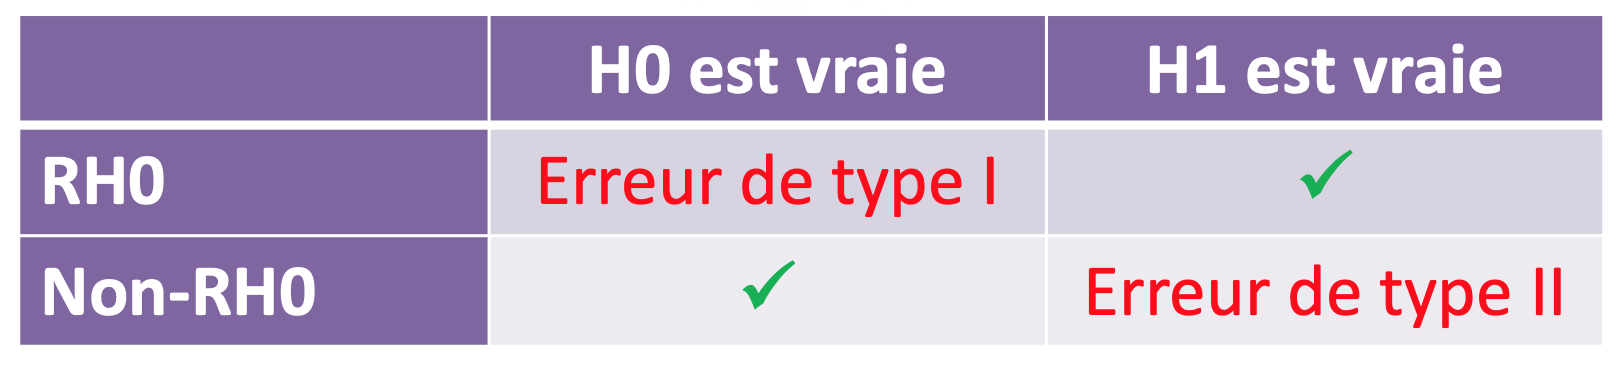
\includegraphics[scale =0.5]{images/errors.png}
    \caption{Deux types d'erreur}
    \label{fig:type_error}
\end{figure}

\subsubsection{Erreur de type I}
Conclure qu’il y a un effet du traitement ($\pi_{A} \neq \pi_{B}$) alors qu’en fait il n’y en a pas($\pi_{A} = \pi_{B}$) =\textbf{faux-positif}

\subsubsection{Erreur de type II}
Conclure qu’il n’y a pas d’effet du traitement ($\pi_{A} = \pi_{B}$) alors qu’en fait il y en a un($\pi_{A} \neq \pi_{B}$) = \textbf{Faux-négatif}

\subsection{Puissance d'un test}
On va plus souvent parler de la puissance d’un test : 
$$Puissance = 1 - \beta$$

plutôt que du risque d’erreur de type II ($\beta$), ce qui est en fait équivalent.\\
$$\beta = P(NRH_{0},H_{1})$$ et $$puissance = P(RH_{0},H_{1})$$

Ainsi, la puissance est la probabilité de rejeter $H0$ si $H1$ est vrai.

\subsection{Test bilatéral versus test unilatéral}

\section{Endpoint binaire}

\begin{figure}[H]
    \centering
    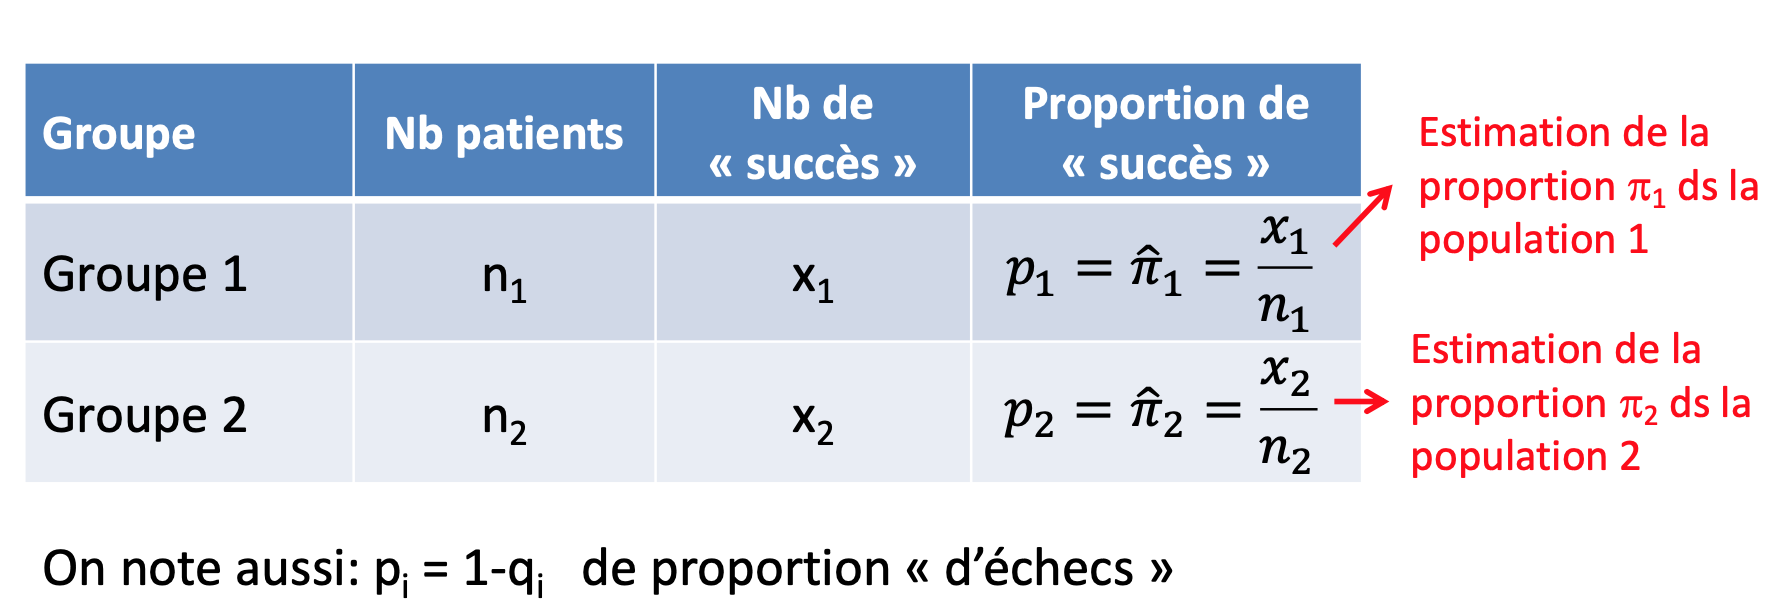
\includegraphics[scale = 0.3]{images/estimationproportion.png}
    \caption{Tableau endpoint binaire}
    \label{fig:my_label}
\end{figure}

Pour calculer de l’intervalle de confiance pour l’estimation d’une probabilité (proportion) sur base de l’approximation normale de la binomiale (sans correction) :
\begin{figure}[H]
    \centering
    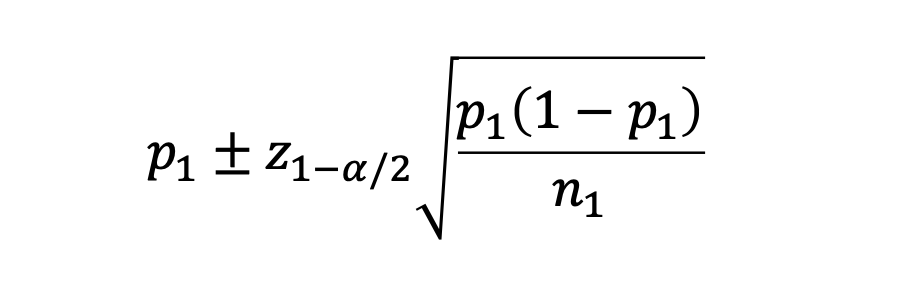
\includegraphics[scale = 0.5]{images/intervalprob.png}
    \caption{intervalle de confiance d'une probabilité (proportion)}
    \label{fig:my_label}
\end{figure}

\begin{figure}[H]
    \centering
    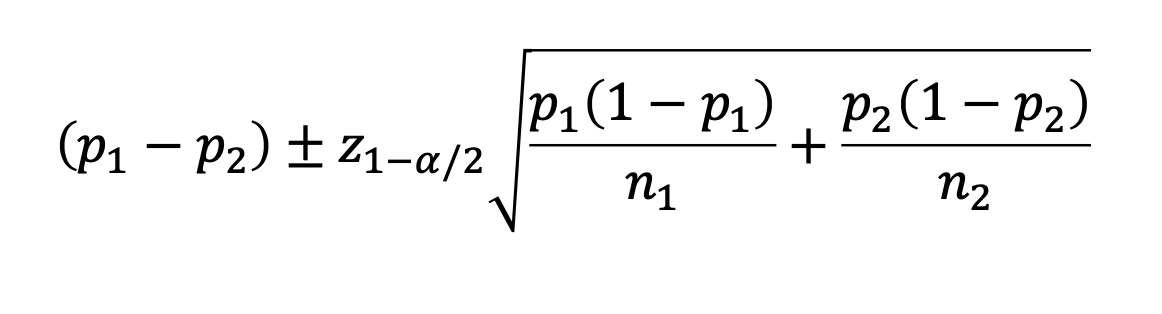
\includegraphics[scale = 0.5]{images/intervaldiffprop.png}
    \caption{intervalle de confiance pour la différence de deux proportions}
    \label{fig:my_label}
\end{figure}


\section{Endpoint continu}
\subsection{Premier cas $\sigma_1^2 \neq \sigma_2^2$}
\begin{figure}[H]
    \centering
    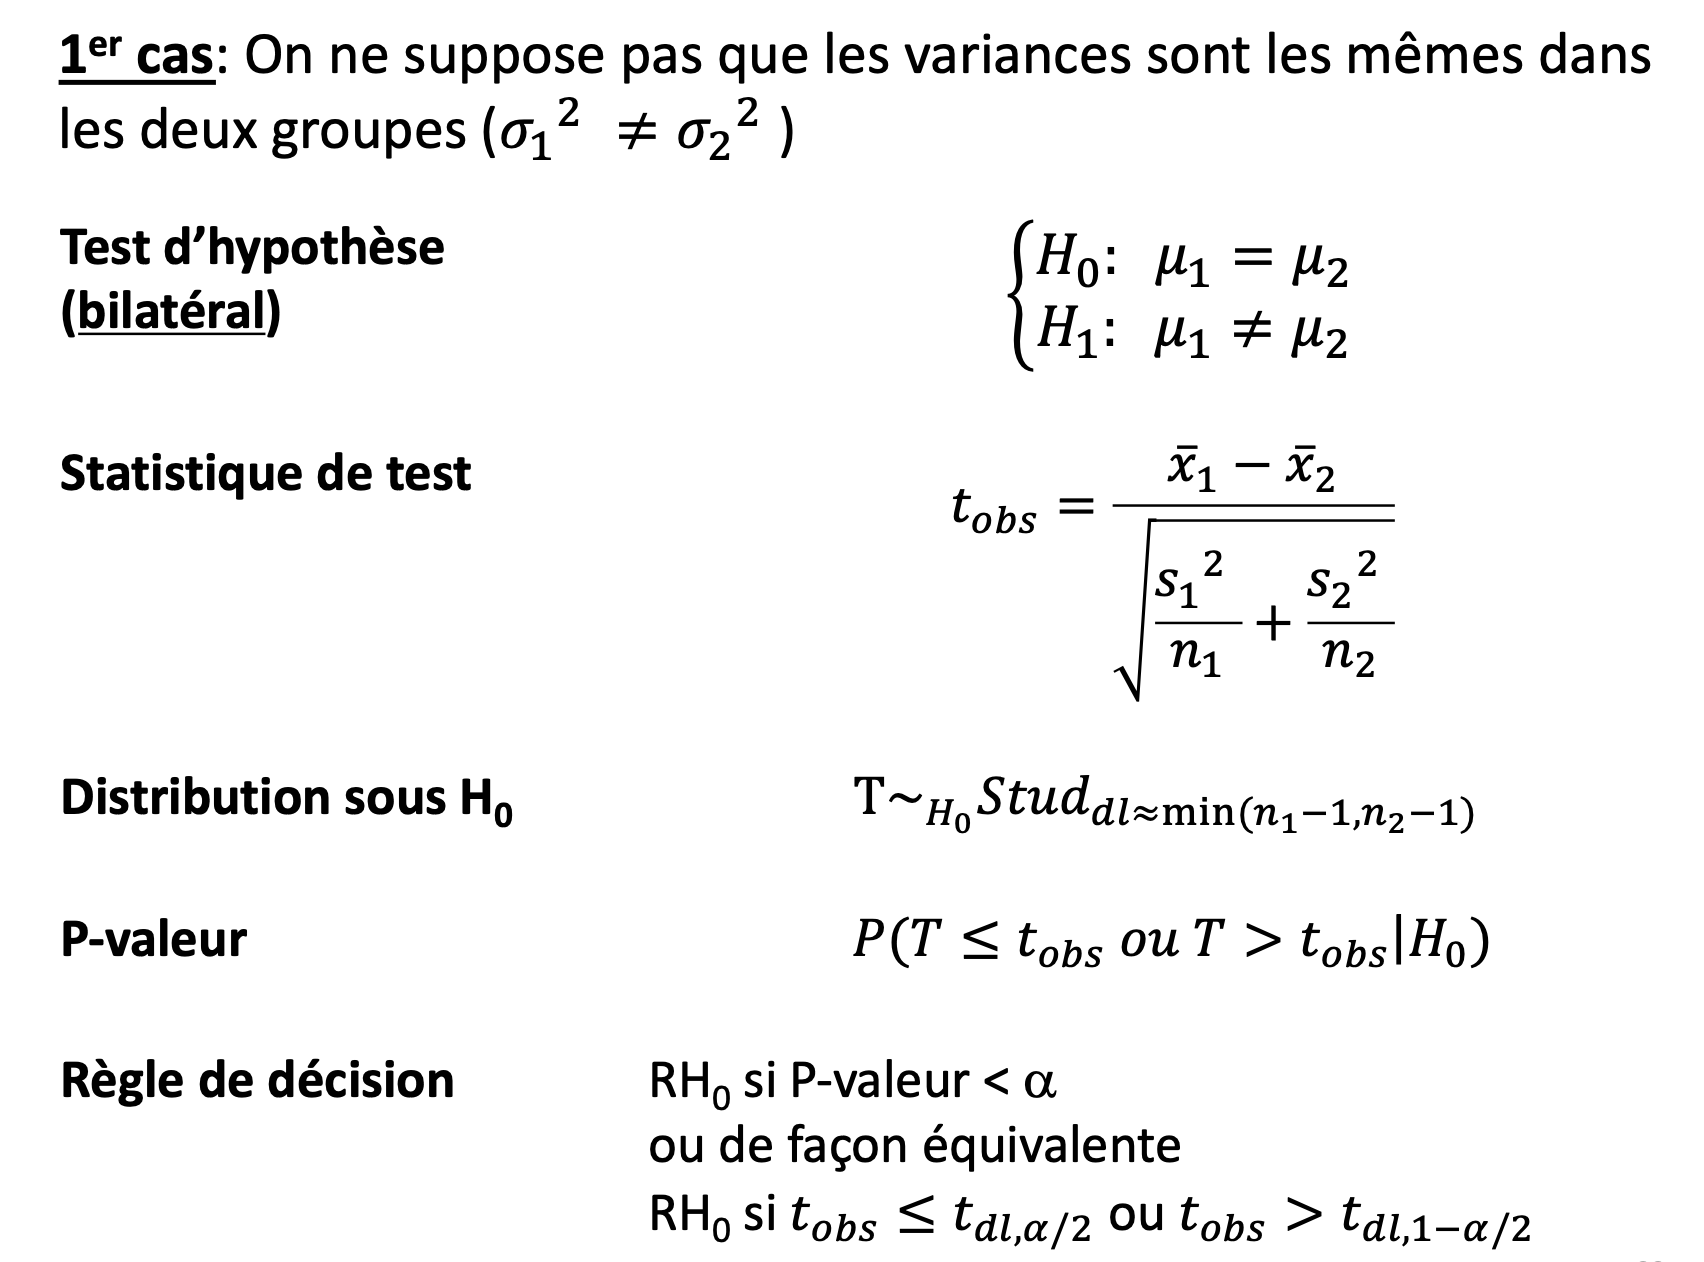
\includegraphics[scale = 0.5]{images/firstcasecontinu.png}
    \caption{Premier cas $\sigma_1^2 \neq \sigma_2^2$}
    \label{fig:my_label}
\end{figure}

\subsection{Deuxième cas $\sigma_1^2 = \sigma_2^2$}
\begin{figure}[H]
    \centering
    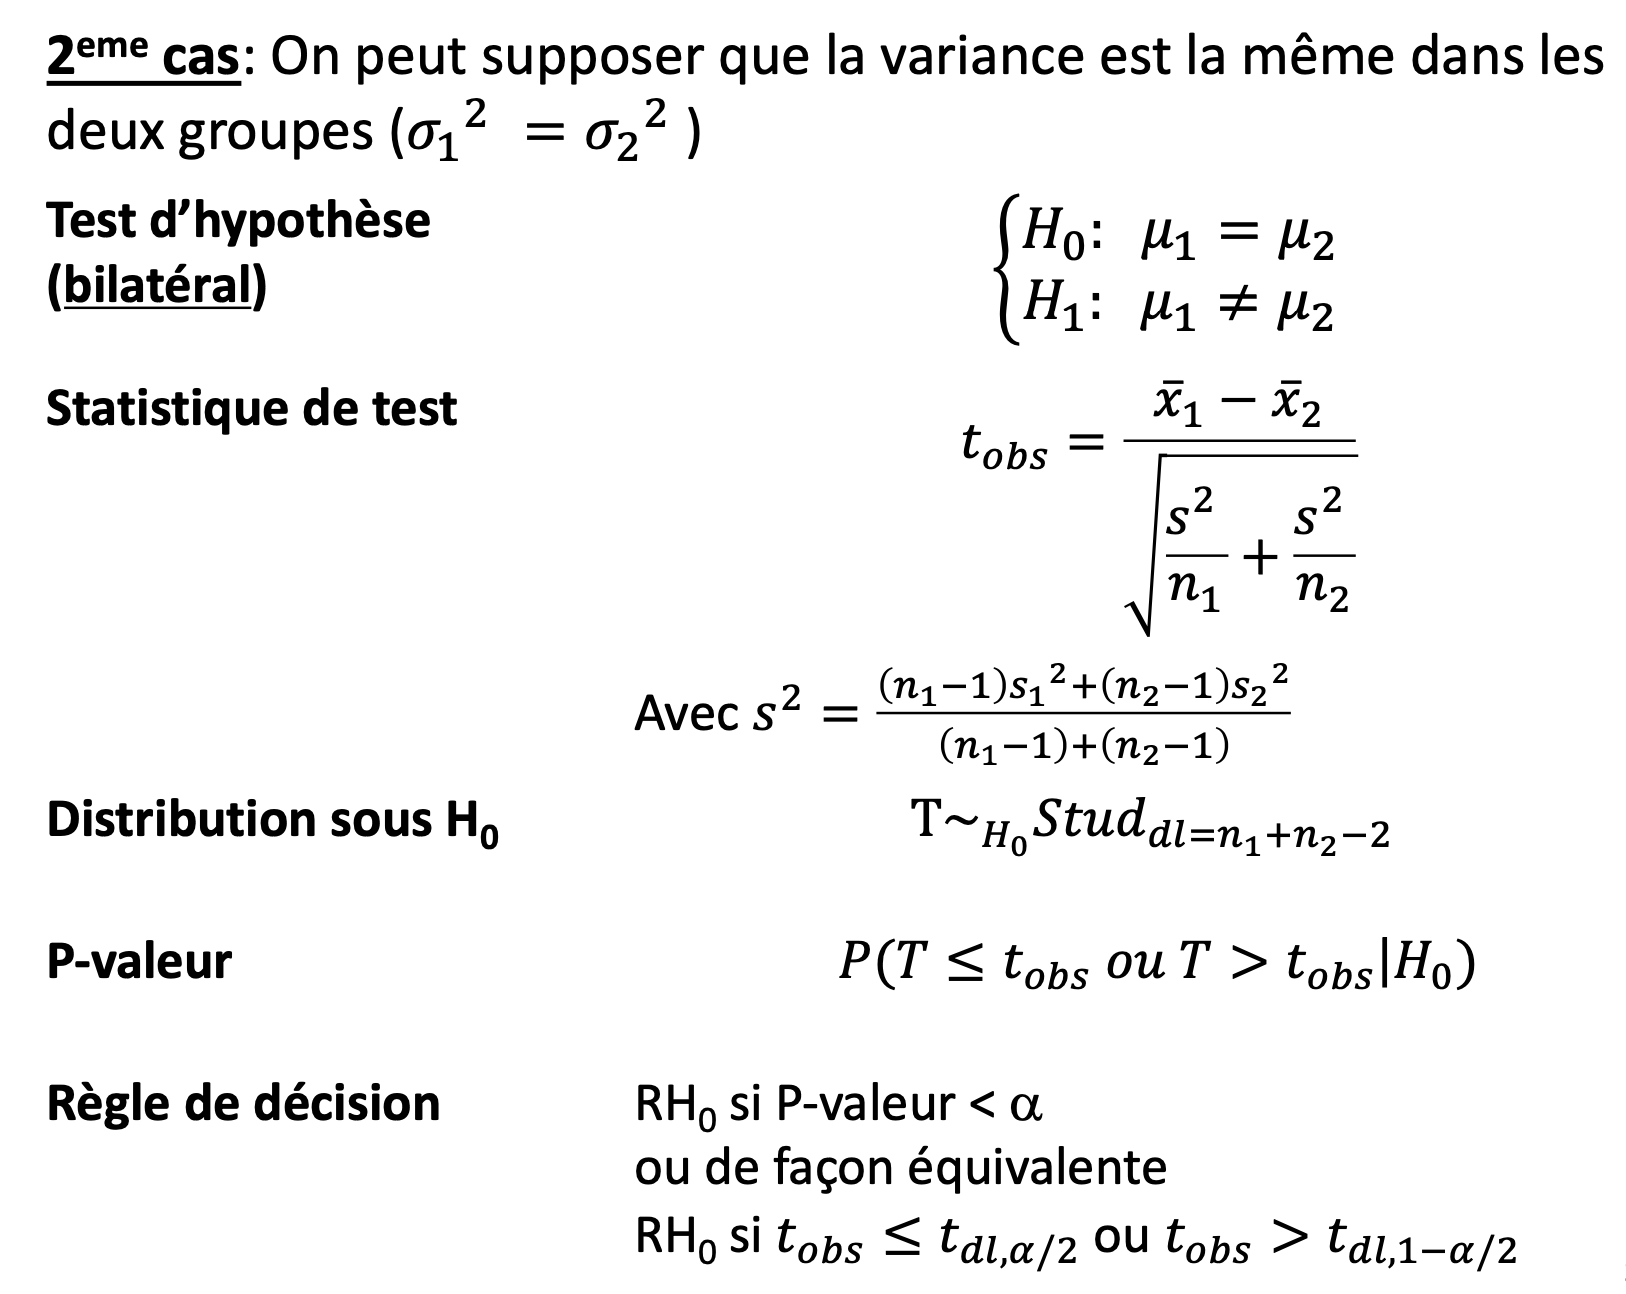
\includegraphics[scale = 0.5]{images/deuxiemecascontinu.png}
    \caption{Deuxième cas $\sigma_1^2 = \sigma_2^2$}
    \label{fig:my_label}
\end{figure}



\chapter{Introduction}

Introduction aux essais cliniques.

\section{Du laboratoire au patient}
Lorsqu'on veut mettre un nouveau médicament sur le marché, on a plein de questions \ref{fig:questions}.

\begin{figure}[H]
    \centering
    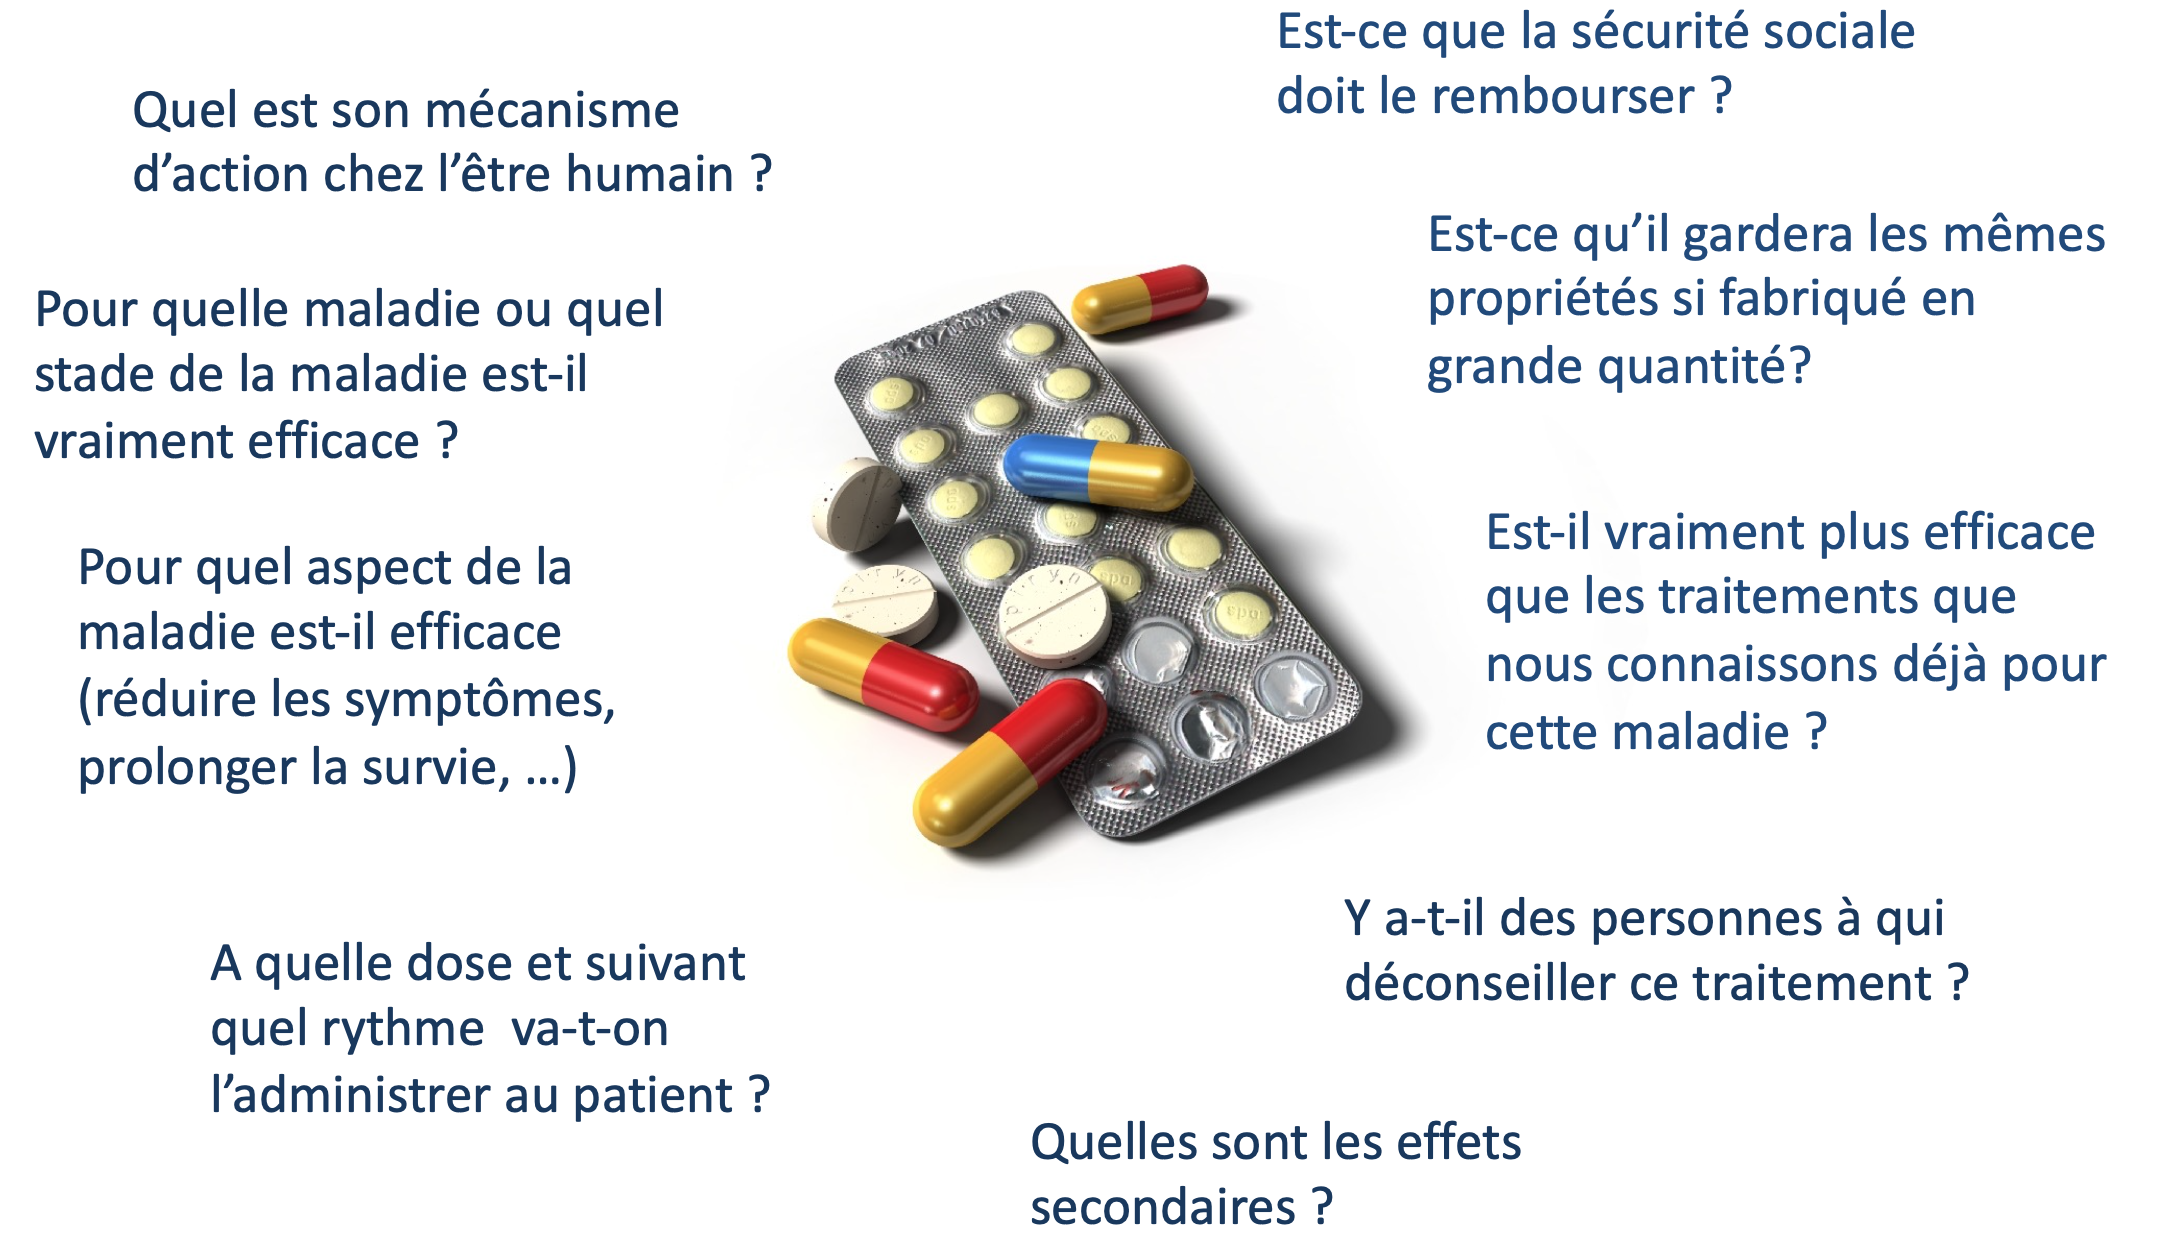
\includegraphics[scale=0.2]{images/questions.png}
    \caption{Questions sur médicament}
    \label{fig:questions}
\end{figure}

La recherche clinique (et préclinique) va tenter d’apporter une réponse à toutes ces questions dans la figure \ref{fig:questions}. La statistique, et plus particulièrement la biostatistique, est un outil fondamental de la recherche clinique.

La recherche clinique se base sur la mise sur pied, la réalisation, l’analyse et la diffusion d’essais cliniques.\\


\textbf{Essai clinique} toute expérience sur des êtres humains visant à déterminer l’impact d’un (ou plusieurs) traitement(s) pour guérir, soigner ou prévenir une maladie.\\

Le plus souvent : Essais cliniques impliquant deux (ou plusieurs) traitements appliqués à deux (ou plusieurs) groupes de personnes ou patients qui sont enrôlés, traités et suivi suivant le même protocole.\\

\textbf{But des essais cliniques :}
\begin{itemize}
    \item Découvrir, étudier et développer de nouveaux traitements pour guérir, soigner ou prévenir une maladie
    \item Fournir suffisamment d’évidence pour changer la pratique clinique dans le traitement d’une maladie spécifique et d’une population spécifique
\end{itemize}

\vspace{0.15cm}
\textbf{ Traitement :}
\begin{itemize}
    \item Un médicament particulier à un certain dosage, une combinaison de médicaments, etc
    \item Une technique chirurgicale, une technique de radiothérapie, etc 
    \item Un régime, des mesures en matière d’hygiène de vie, une
campagne de prévention, etc
    \item Une stratégie de traitements (combinaison de différentes approches)
\end{itemize}


\subsection{Déclaration d’Helsinki}
Cela correspond aux droits du patient. C'est l'énoncé des principes éthiques applicables à la recherche médicale impliquant des êtres humains. Les objectifs de la recherche médicale ne doivent jamais prévaloir sur les droits des personnes impliquées.


\subsection{Comité d’éthique et Consentement éclairé}

Tous les protocoles de recherche impliquant des êtres humains doivent être revus et approuvés par le board institutionnel et le comité d’éthique (CE) avant de pouvoir démarrer. Ces comités restent impliqués tout au long de l'étude et tout événement inattendu arrivant durant le cours d’un essai doivent leur être signalés.\\

Les patients éligibles ne peuvent être enrôlés dans un essai clinique seulement une fois :
\begin{itemize}
    \item qu’ils ont été informés que leur participation n’est pas obligatoire, et qu’une fois enrôlés ils peuvent quitter l’essai à tout moment
    \item qu’ils ont été informés des risques et des bénéfices de leur participation dans l'essai clinique avec suffisamment de détails
    \item qu’ils ont signé un \textbf{consentement éclairé} pour leur participation.

\end{itemize}

\section{Essais Cliniques : principe}
Les différentes étapes sont :
\begin{enumerate}
    \item Protocole : objectif, méthodologie
    \item Sélections des centres, des investigateurs, accord du CE
    \item Sélections et traitement de patients
    \item Encodage des données
    \item Analyse statistiques des données
    \item Publication/présentation des résultats.
\end{enumerate}
\vspace{0.15cm}
Le biostatisticien va jouer un rôle dans plusieurs étapes. Il est impliqué dans la mise en place du protocole, dans l'analyse statistique et dans la publication des résultats. 

\subsection{Effet traitement}
\textbf{L’effet d’un traitement} pour un patient est la différence entre ce qu’il est arrivé au patient suite à l’administration de ce traitement et ce qu’il serait arrivé à ce patient s’il n’avait pas reçu ce traitement. (Senn, 1999)\\

Les points importants sont : 
\begin{itemize}
    \item Idée de comparaison : effet du traitement est toujours comparatif ! \item Effet du traitement 1 Activité du traitement
    \item Notion de CAUSALITÉ !
\end{itemize}
\vspace{0.15cm}
Différents effets peuvent influencer la maladie sans que ce soit le médicament. Il faut les prendre en compte.\\

\begin{itemize}
    \item Cours naturel de la maladie 
    \item \textbf{Facteurs confondant} (exemple Glace-noyade)
    \item Effet de sélection
     \item \textbf{ Régression to the mean} (exemple avec performance extraordinaire et faible probabilité de la répéter)
     \item ...
\end{itemize}
\vspace{0.15cm}
La question importante est \textbf{Comment établir la causalité ?}\\

Pour répondre « OUI » sans ambiguïté, il faut que les deux
groupes soient comparables en tout point : même âge, même
pronostique, même niveau socio-économique, ….

\subsection{Randomisation}
Le choix du traitement est alloué au hasard aux différents patients.\\
\begin{itemize}
    \item Comparaison non biaisée des traitements
    \item Variables confondantes distribuées également entre les groupes
    \item Base de l’inférence statistique
\end{itemize}
\vspace{0.15cm}
\textbf{Principe de base} : randomisation totalement aléatoire\\
\begin{itemize}
    \item Chaque patient à la même chance de recevoir chacun des
traitements étudiés
    \item L’assignement d’un patient à un groupe traitement n’influence pas le choix du traitement des autres patients
    \item On ne sait pas à l’avance quel traitement chacun des patients va recevoir.
\end{itemize}
\vspace{0.15cm}
\textbf{La randomisation des patients entre les différents traitements n’est éthiquement acceptable que :}\\
\begin{itemize}
    \item si le médecin (et de façon générale la communauté scientifique) est en état d’équipoise.

\item si un traitement efficace est connu, mais que les conséquences d’un traitement de contrôle sans traitement sont réversibles et modérées (par exemple mal de tête) et que le ratio risque-bénéfice peut justifier l’essai clinique.
\end{itemize}

\subsection{Réponse (Outcome)}

Les effets du traitement sont évalués en mesurant une ou plusieurs caractéristiques sur les patients = \textbf{variable(s) que l’on va étudier}\\

\textbf{Remarques}\\

\begin{itemize}
    \item Endpoint principal et endpoints secondaires
    \begin{itemize}
        \item  L’\textbf{endpoint principal} sera utilisé pour le calcul de taille
d’échantillon et pour les conclusions principales de l’étude
\item Les \textbf{endpoints secondaires} seront utilisés pour
confirmer/appuyer les conclusions tirées sur base de
l’endpoint principal
    \end{itemize}
\item Le choix de l’endpoint principal (et des endpoints secondaires)
est crucial et doit rencontrer un consensus
\item Uniformisation des mesures pour diminuer la variabilité
\end{itemize}
\vspace{0.15cm}
\textbf{Comment généraliser ces résultats à d’autres patients que ceux dans l’essai clinique ?}\\

On fait des tests cliniques sur un sous groupe de la population et on fait une extrapolation.
\subsection{Extrapolation}
Pour pouvoir faire de l’inférence(=interpolation) il faut que l’échantillon soit :
\begin{itemize}
    \item  En théorie : ALÉATOIRE
    \item En pratique : REPRÉSENTATIF de la population
\end{itemize}
\vspace{0.15cm}
Pour s’assurer de la représentativité de l’échantillon, les patients entrés dans l’essai clinique devrait être un échantillon aléatoire de la population étudiée. Mais Impossible pour des raisons éthiques et pratiques. Les patients entrés dans l’essai clinique doivent être
représentatifs de la population étudiée(problème de sous représentativité des minorités ethniques dans les essais cliniques).\\

\textbf{Si on s’intéresse à l’effet d’un nouveau traitement, peut-on directement commencer un tel essai clinique ?}
 Non on a des phases bien précises à respecter. Ces phases permettent de collecter des informations sur la posologie, la dose, les mécanismes d'action et l'activité du traitement, les effets secondaires, ....
 
 \subsection{Différentes phases}
 \subsubsection{Phases avant expérimentation clinique}
 On a deux phases avant les expérimentations cliniques : \textbf{recherche de base} qui se fait in vitro en laboratoire et \textbf{expérimentation préclinique} qui se fait in vivo dans des animaux.
 
\subsubsection{phase I}

\begin{enumerate}
    \item 1ère administration à des êtres humains 
    \item < 100 patients, 10-30 patients
    \item Action de la molécule ("bio-chimique") 
    \item Profil de toxicité
    \item Dose(s) recommandée(s)
\end{enumerate}

\subsubsection{phase II}

\begin{enumerate}
    \item  1ère évaluation de l’activité chez des êtres humains (en général : affectés par la maladie)
    \item<100 patients, 40-80 patients
    \item Profile de toxicité
    \item Dose
    \item Réponse, mécanisme d’action
\end{enumerate}

\subsubsection{phase III}

\begin{enumerate}
    \item  Évaluation comparative de l’efficacité
    \item Plusieurs centaines/milliers de patients
    \item Toxicité
    \item Efficacité
\end{enumerate}

\subsubsection{phase IV}
\begin{itemize}
    \item Follow-up à long-terme (efficacité et safety) dans des conditions plus proches de la réalité, et a plus grande échelle
    \item « pharmacosurveillance » : Peut permettre de mettre en évidence des effets
secondaires rares
    \item Obtenir des données supplémentaires pour les négociations sur le cout et le remboursement possible
    \item Typiquement plusieurs milliers de patients traités dans des conditions beaucoup moins contrôlées
\end{itemize}
\subsubsection{Remarques}
\begin{itemize}
    \item Plusieurs essais sont en général réalisés pour une même phase. Ces phases ne sont pas toujours aussi distinctes.
    \itemTout au long du processus Phase I-Phase III : les aspects « commerciaux », « techniques », et « marketing » sont évalués en parallèle.
\item Après complétion de la phase III : soumission aux autorités pour autorisation de mise sur le marché
\end{itemize}
\section{Documents}

\subsection{Protocole}

\textbf{Protocole} : Document rédigé et approuvé avant le début de l’étude et ayant pour but de \textbf{standardiser} la façon dont est menée l’étude. Il contient les points suivants :
\begin{itemize}
    \item Motivation de l’étude, connaissances actuelles
\item Objectif(s) - Question(s) d’intérêt clairement définie(s)
 \begin{itemize}
     \item Objectif principal/Objectifs secondaires
     \item Hypothèses statistiques
 \end{itemize}
\item Outcomes/Mesures de réponse
\begin{itemize}
    \item Outcome principal / secondaires
\end{itemize}
\item Définition de la population cible, échantillonnage et taille d’échantillon
\item Phase, design de l’étude, randomisation.
\item Traitements considérés
\begin{itemize}
    \item Informations disponibles sur ce traitement
    \item Mode d’administration, dosage et posologie
\end{itemize}

\item Prise en charge des patients et collecte des
données
\begin{itemize}
    \item Gestion des effets secondaires, réduction des
doses, traitement concomitant, autres soins, …
\item Examens, visites et données à collecter 
\end{itemize}
\item Technique d’analyse des résultats
\begin{itemize}
    \item En fonction des objectifs, du plan d’expérience et
de la variable d’outcome
\item Monitoring statistique de l’essai
\end{itemize}
\item …
\end{itemize}
\vspace{0.15cm}
La population de l'essai clinique se définit dans le protocole sur base d’une liste de critère d’éligibilité (= liste de critères d’inclusion et de non-inclusion permettant de
définir précisément les patients pouvant être randomisés dans
l’essai clinique.)

\subsection{Plan d’analyse Statistique}

Document rédigé et approuvé avant que le statisticien ait accès aux données de l’étude.\\

\begin{itemize}
    \item SAP en anglais (Statistical Analysis Plan)
    \item Peut être une partie du protocole ou un document séparé
    \item A pour but principal d’éviter le « qui cherche trouve » 
     \item Toutes les analyses statistiques prévues doivent être pré- spécifiée dans le SAP. Les analyses non pré-spécifiées dans le SAP seront interprétées comme « exploratoires »
    \item Clairement le type d’analyse dépendra du choix de l’endpoint et des objectifs de l’étude. Ces techniques d’analyse doivent être conformes aux recommandations faites dans les guidelines internationales.
\end{itemize}\\

Ce doucement doit détailler :

\begin{itemize}
    \item Les patients inclus dans chaque analyse (« Intent-toTreat » ou du
«Per-protocol »)
\item Le niveau « d’importance » de chaque analyse (primary,
secondary, supportive, exploratory, …)
\item Les méthodes statistiques utilisées, et notamment
\begin{itemize}
    \item  Les tests d’hypothèse et le niveau a à utiliser pour
l’interprétation de ces tests
\item Les modèles statistiques, facteurs inclus dans ces modèles,
facteurs de stratification
\item La gestion des données manquantes
\item …
\end{itemize}
\item …
\end{itemize}

\subsection{Patients inclus dans l’analyse [Analysis set]}
Lorsqu'on fait l'analyse statistique, différentes techniques peuvent être utilisées pour prendre en compte la population de patients.\\

\textbf{Intention-to-treat (ITT) set:}
Tous les patients randomisés sont inclus dans l’analyse, dans le groupe de traitement auquel ils ont été randomisés. Même si certains arrêtent avant, on les prend en compte dans le groupe où ils ont été placés lors de la randomisation.\\
Cette. technique est la plus défavorable, mais si elle permet de prouver l'efficacité du traitement, c'est le JACKPOT.\\

\textbf{Per Protocol (PP) set:}
On prend le sous-ensemble de patients définis dans le protocole. On va souvent exclure les patients inéligibles, les patients n’ayant pas commencé le traitement, etc. On Analyse les patients dans le groupe correspondant au traitement reçu et non pas au traitement assigné par randomisation.\\

\textbf{Safety set:}
On prend en compte que les patients utilisés pour analyse les aspects «safety » du traitement (par exemple effets indésirables). En général, cela ne concerne que les patients ayant commencé le traitement.

\subsection{Types d’analyses}

\subsubsection{Main/Primary Analysis}
Analyse principale de l’endpoint principal. C'est cette analyse qui dirige nos tests statistiques.

\subsubsection{Secondary Analyses}
Analyse principale des endpoints secondaires. Cela permet de mettre en évidence certaines conclusions.

\subsubsection{Supportive/Sensitivity Analyses}
Analyse des endpoints primaires/secondaires sur un autre analysis set, ou avec des techniques d’analyse un peu différente. On utilise cela pour faire des études sur des sous-groupes. 

\subsubsection{Safety Analyses}
\begin{itemize}
    \item Analyse principale des toxicités, effets secondaires,
indésirables, etc
    \item Sur base du Safety Set
    \item Doit dans l’idéal aussi rapporter l’exposition au traitement des patients (par exemple nombre de doses reçues)
\end{itemize}\\
\begin{center}
\fbox{%
\begin{minipage}{0.75\textwidth}
Les conclusions de l’analyse statistique d’un essai clinique ne seront valides que si l’essai clinique a été correctement mis sur pied.
\end{minipage}
}
\end{center}


\section{Quelques remarques}
Le premier essai clinique randomisé « moderne » a été conduit par le Medical Research Council (UK) dont le principal leader était le statisticien Austin Bradford Hill (1897-1991).
 
\chapter{Phase III - design}

La phase III est la dernière phase du développement clinique d’un nouveau traitement.\\

Les phases III sont toujours des \textbf{essais comparatifs}:
\begin{itemize}
    \item L’idée est de confronter le nouveau traitement au traitement
standard ou à un placebo
    \item L’idée est que les patients du groupe traitement et du groupe
contrôle ne diffère que par leur traitement (\textbf{causalité}).
\end{itemize}

\section{Choix de l’endpoint}

Le choix de l’endpoint est très important et doit se faire en fonction de l’objectif de l’étude. Il est déterminé en fonction du type de maladie et du type de
patients et doit représenter un bénéfice clinique pour le patient. Ce choix va déterminer le type d’analyse. 

\subsection{Primary endpoint}
\begin{itemize}
    \item Endpoint principal
    \item En général : unique, base pour calcul de la taille d’échantillon
    \item De préférence : "Hard" endpoint
\end{itemize}

\subsection{Secondary endpoints}
\begin{itemize}
    \item Endpoints secondaires
     \item En général : plusieurs, attention à la puissance
\end{itemize}


\section{Choix du groupe contrôle}
Lors d'essais cliniques, on fait une comparaison du traitement avec un autre traitement (= traitement de référence) sur une même période, un groupe similaire de patients, et dans des conditions similaires.\\

\begin{center}
    \textbf{Que peut-on considérer comme bras contrôle ?}
\end{center}
\begin{itemize}
    \item un groupe de patients non-traité ?
 \item un groupe de patients traités avec un placebo
 \item un groupe de patients avec un autre traitement connu ?
 \item un groupe de patients avec un autre traitement expérimental ? (Besoin d'un autre groupe de contrôle quand même)
\end{itemize}

\subsection{Unités témoins ou groupe de références}
ensemble des individus servant de comparaisons et qui ne reçoit pas de traitement (ou un placebo) ou qui reçoit un traitement dont les effets sont connues(« traitement standard »)

\subsection{Placebo}

\textbf{Placebo}: substance ayant le même aspect (forme, odeur, couleur, etc) que le traitement étudié, mais étant totalement inactive.

\subsubsection{Effet placebo}
L’effet placebo est souvent lui-même un effet confondant : une personne recevant un placebo, en pensant recevoir une substance active, peut se sentir mieux – simplement parce qu’on lui a administré quelque chose qu’elle croit actif (effet placebo – du latin « je plais »).

\subsubsection{Étude en aveugle}
Étude en aveugle avec un contrôle placebo : on randomise une partie des unités expérimentales à recevoir le traitement étudié et l’autre partie à recevoir un placebo sans que l’unité expérimentale (ou son entourage) ne sache quel traitement a été attribué à quelle unité expérimentale.\\

Il y a \textbf{trois niveaux d'aveugle : }
\begin{figure}[H]
    \centering
    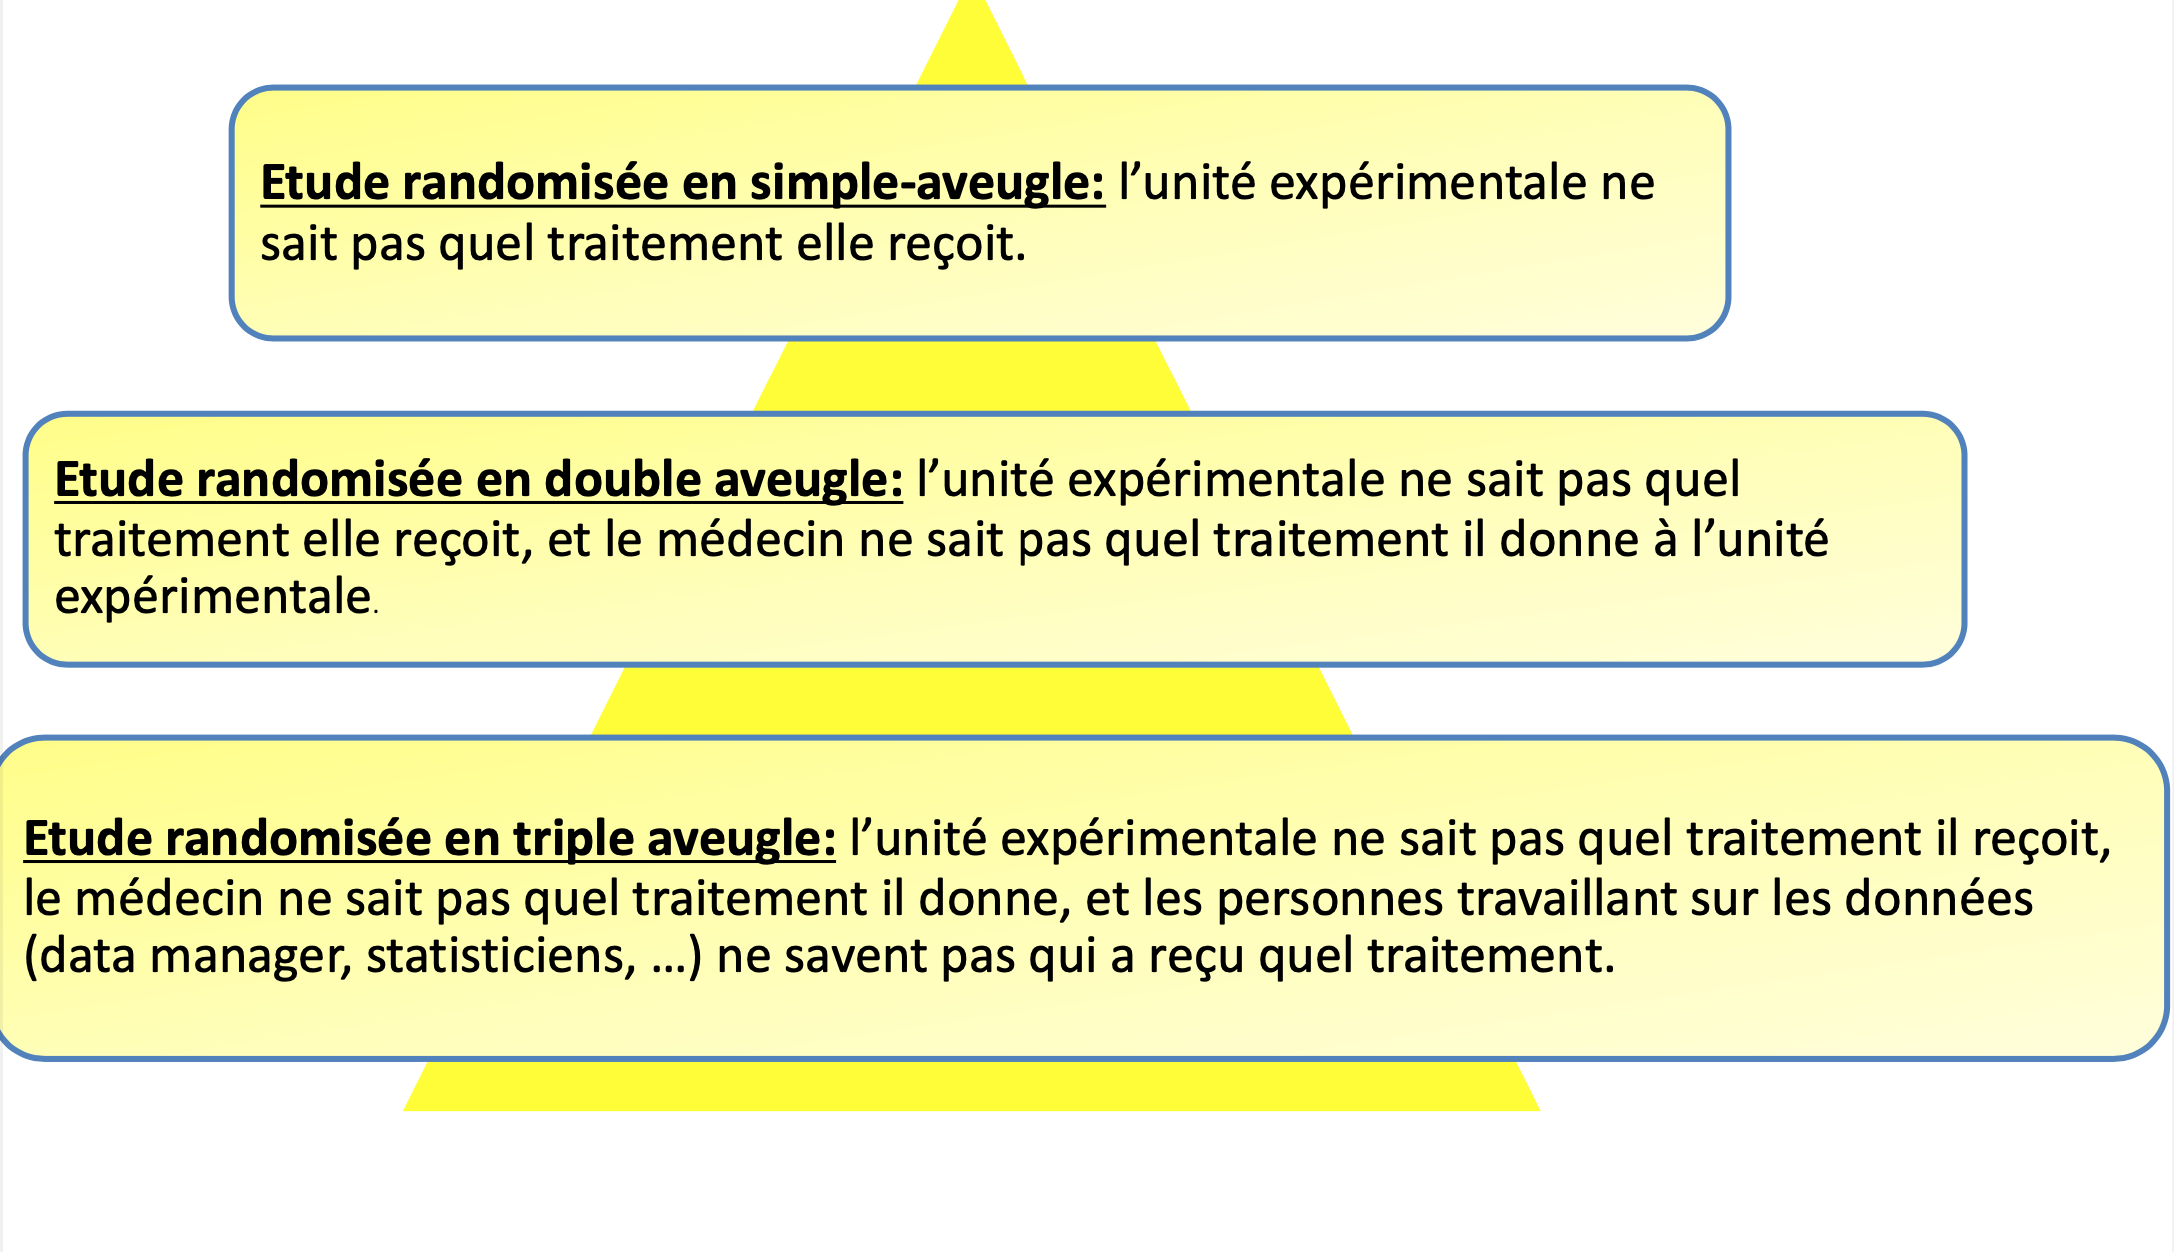
\includegraphics[scale = 0.3]{images/3_blind_levels.png}
    \caption{trois niveaux d'aveugle}
    \label{fig:my_label}
\end{figure}
\begin{enumerate}
    \item  Étude randomisée en simple-aveugle : l’unité expérimentale ne sait pas quel traitement elle reçoit
    \item  Étude randomisée en double aveugle: l’unité expérimentale ne sait pas quel traitement elle reçoit et le médecin ne sait pas quel traitement il donne à l’unité expérimentale.
    \item Étude randomisée en triple aveugle : l’unité expérimentale ne sait pas quel traitement il reçoit, le médecin ne sait pas quel traitement il donne et les personnes travaillant sur les données (data manager, statisticiens, etc) ne savent pas qui a reçu quel traitement.
    
\end{enumerate}
\vspace{0.15cm}



\textbf{\textit{Pourquoi masquer le traitement au patient ?}}\\

Masquer le traitement au patient : balancer l’effet placebo/essais clinique, éviter que le patient ne change de comportement en fonction du treatment, et éviter un découragement du patient si pas randomisé dans le bras souhaité.\\


\textbf{\textit{Pourquoi masquer le traitement à l’équipe médicale ?}}\\


Masquer le traitement à l’équipe médicale  permet de s’assurer que tous les patients seront traités et suivi de la même façon
– Par exemple management des effets secondaires et toxicités, réalisation
d’examens supplémentaires, soutien au patient, collection des
données, évaluation de l’outcome...\\

\textbf{\textit{Pourquoi masquer le traitement à l’équipe responsable de l’essai clinique ?}}\\
Masquer le traitement à l’équipe responsable de l’essai clinique : s’assurer que les décisions prises au cours de l’essai seront prises indépendamment du traitement reçu par le patient, permet d’éviter un suivi de l’effet traitement au cours de l'essai.

Quand on fait un test pas en aveugle. Il peut être difficile, à la fin de l’étude, de conclure si l’effet observé est dû à un réel effet du traitement ou a un effet du placebo. Alors que si l'étude se fait en aveugle. À la fin de l’étude, on peut conclure que  l’effet observé est dû à un effet réel du traitement (puisque l’effet placebo sera le même dans les deux groupes). Par contre, on ne peut pas évaluer l’effet traitement global.\\

\textbf{\textit{Si on est dans une situation ou l’utilisation d’un placebo est éthique, est-ce vraiment toujours possible ?}}\\

Non ce n'est pas toujours possible pour différentes raisons :
\begin{itemize}
    \item Les études avec placebo sont plus compliquée (et plus couteuse) à mettre sur pied
 \item peuvent avoir un recrutement plus difficile (les gens ne veulent pas recevoir de placebo)
 \item ne sont pas toujours possibles :
 \begin{itemize}
     \item soit, car il est impossible de fabriquer un placebo
\item soit parce que l’administration d’un placebo ne serait pas 
éthique
\item soit parce qu’il n’est pas possible de maintenir l’aveugle
 \end{itemize}
 \item ne sont pas toujours utile par exemple si : 
 \begin{itemize}
     \item on considère une maladie pour laquelle l’effet placebo est 
négligeable (cancer, malformation cardiaque, …)
\item l’effet placebo est négligeable sur la mesure utilisée pour 
mesurer l’effet traitement (réduction de la taille de la tumeur, 
survie, …)
\item on peut raisonnablement penser qu’aucun effet placebo n’est 
attendu.
 \end{itemize}
\end{itemize}
\vspace{0.15cm}

Dans certaines situations, il n'est pas éthique de prendre un placebo. Dans le cas où il existe un traitement connu, et qu'il prévient des dommages graves (décès ou morbidités non réversibles).

\begin{figure}[H]
    \centering
    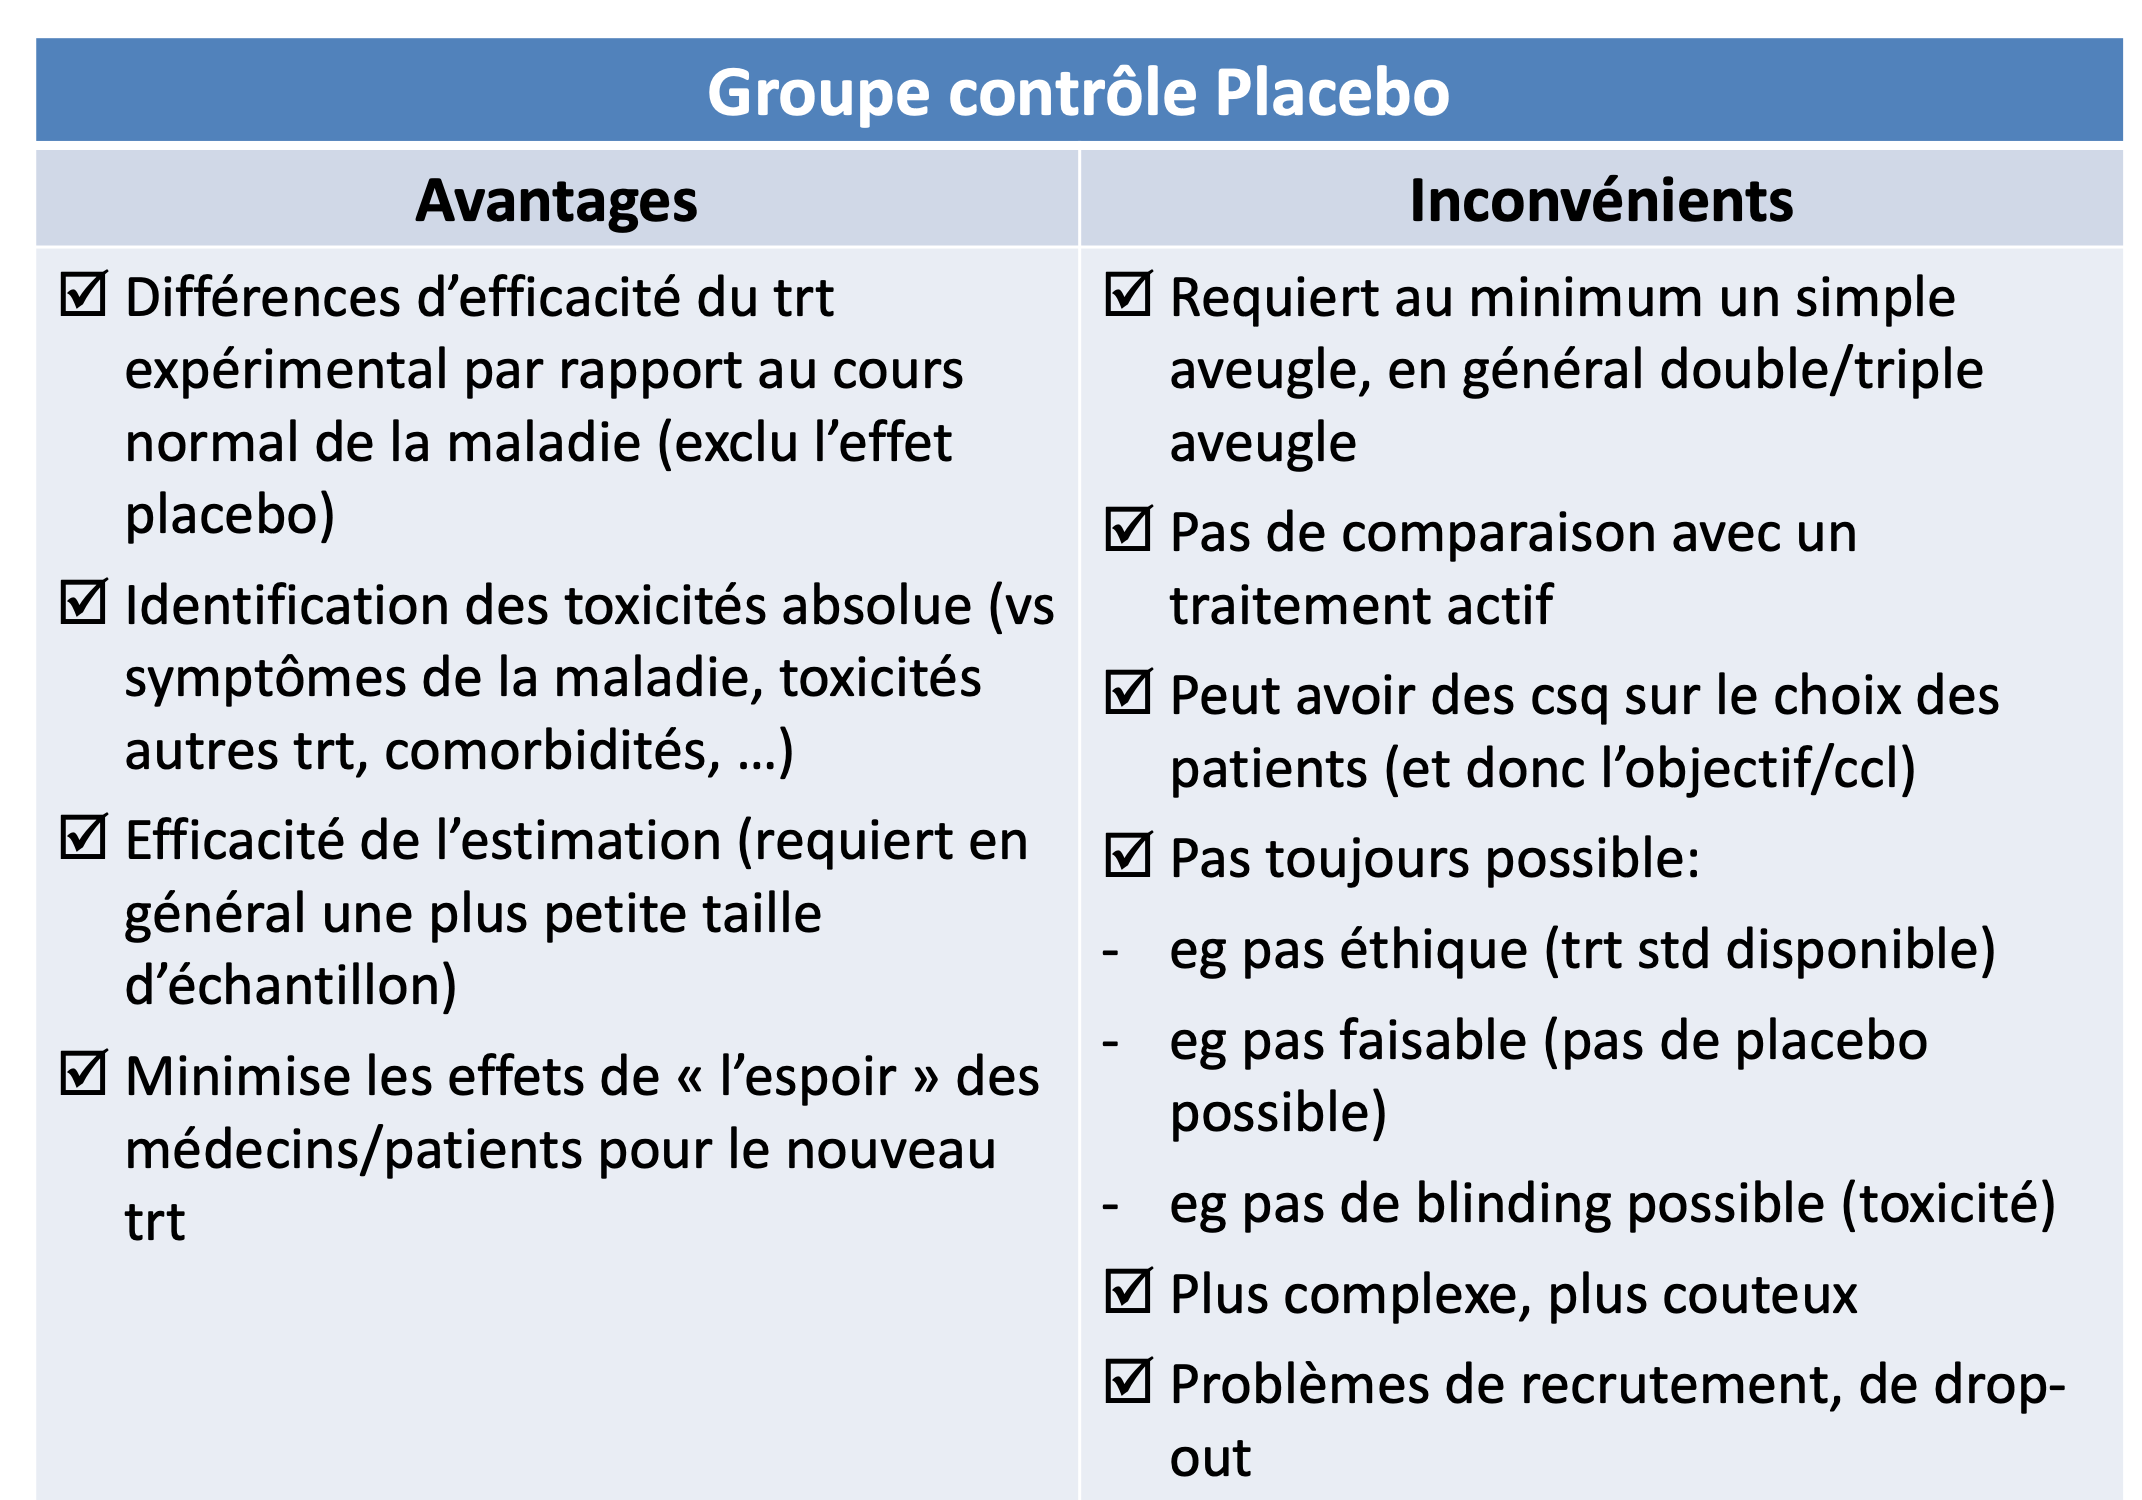
\includegraphics[scale=0.3]{images/placebo.png}
    \caption{}
    \label{fig:my_label}
\end{figure}

\begin{figure}[H]
    \centering
    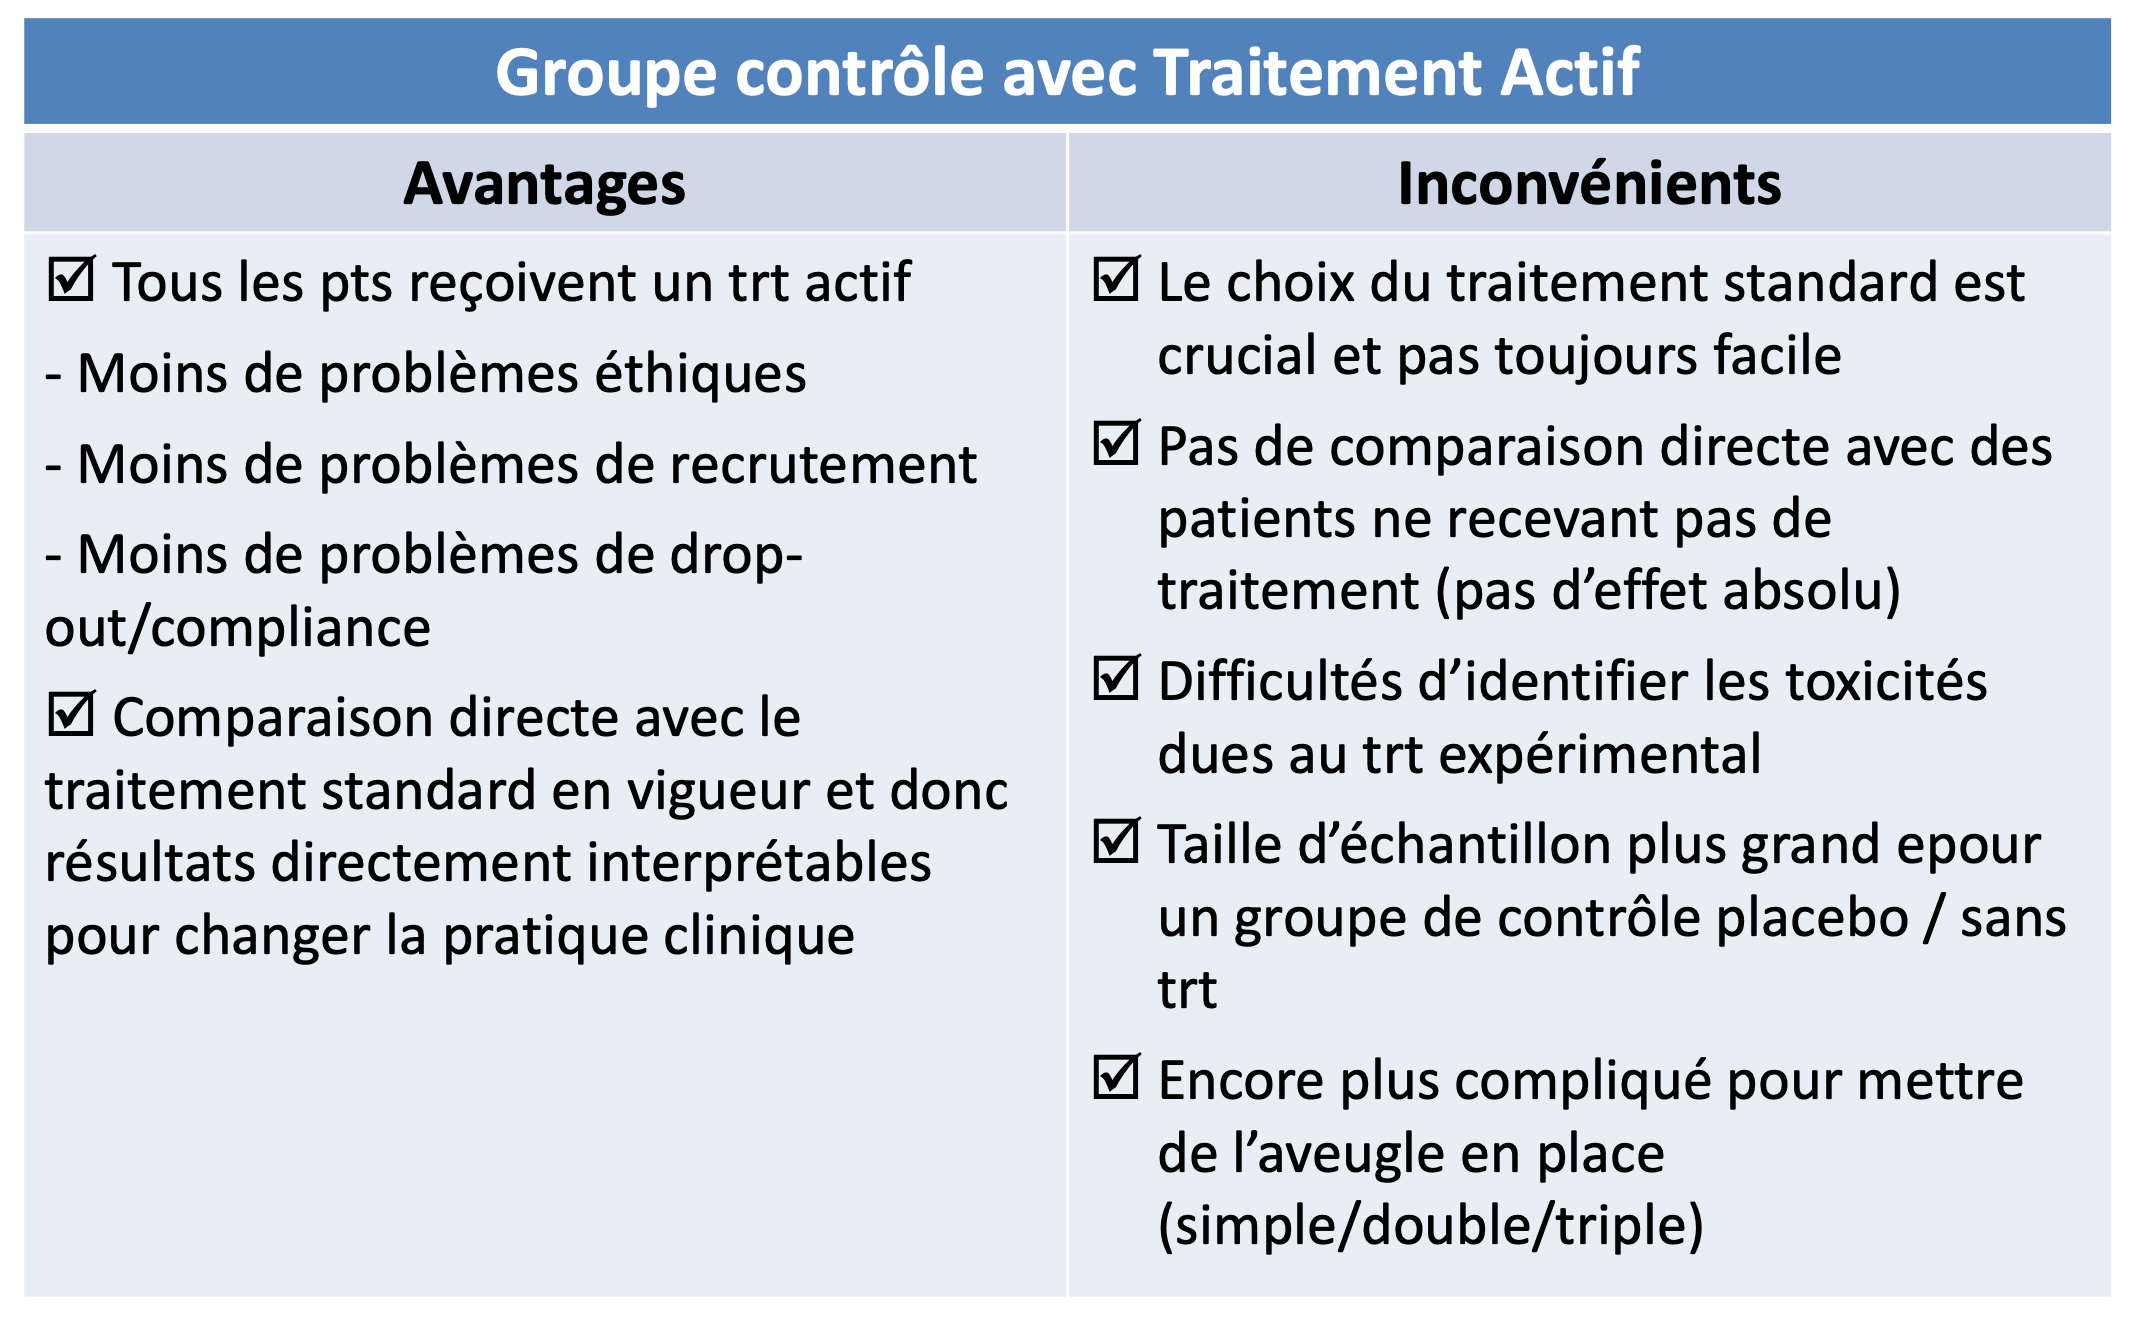
\includegraphics[scale=0.3]{images/actif_treatment.png}
    \caption{}
    \label{fig:my_label}
\end{figure}


\begin{figure}[H]
    \centering
    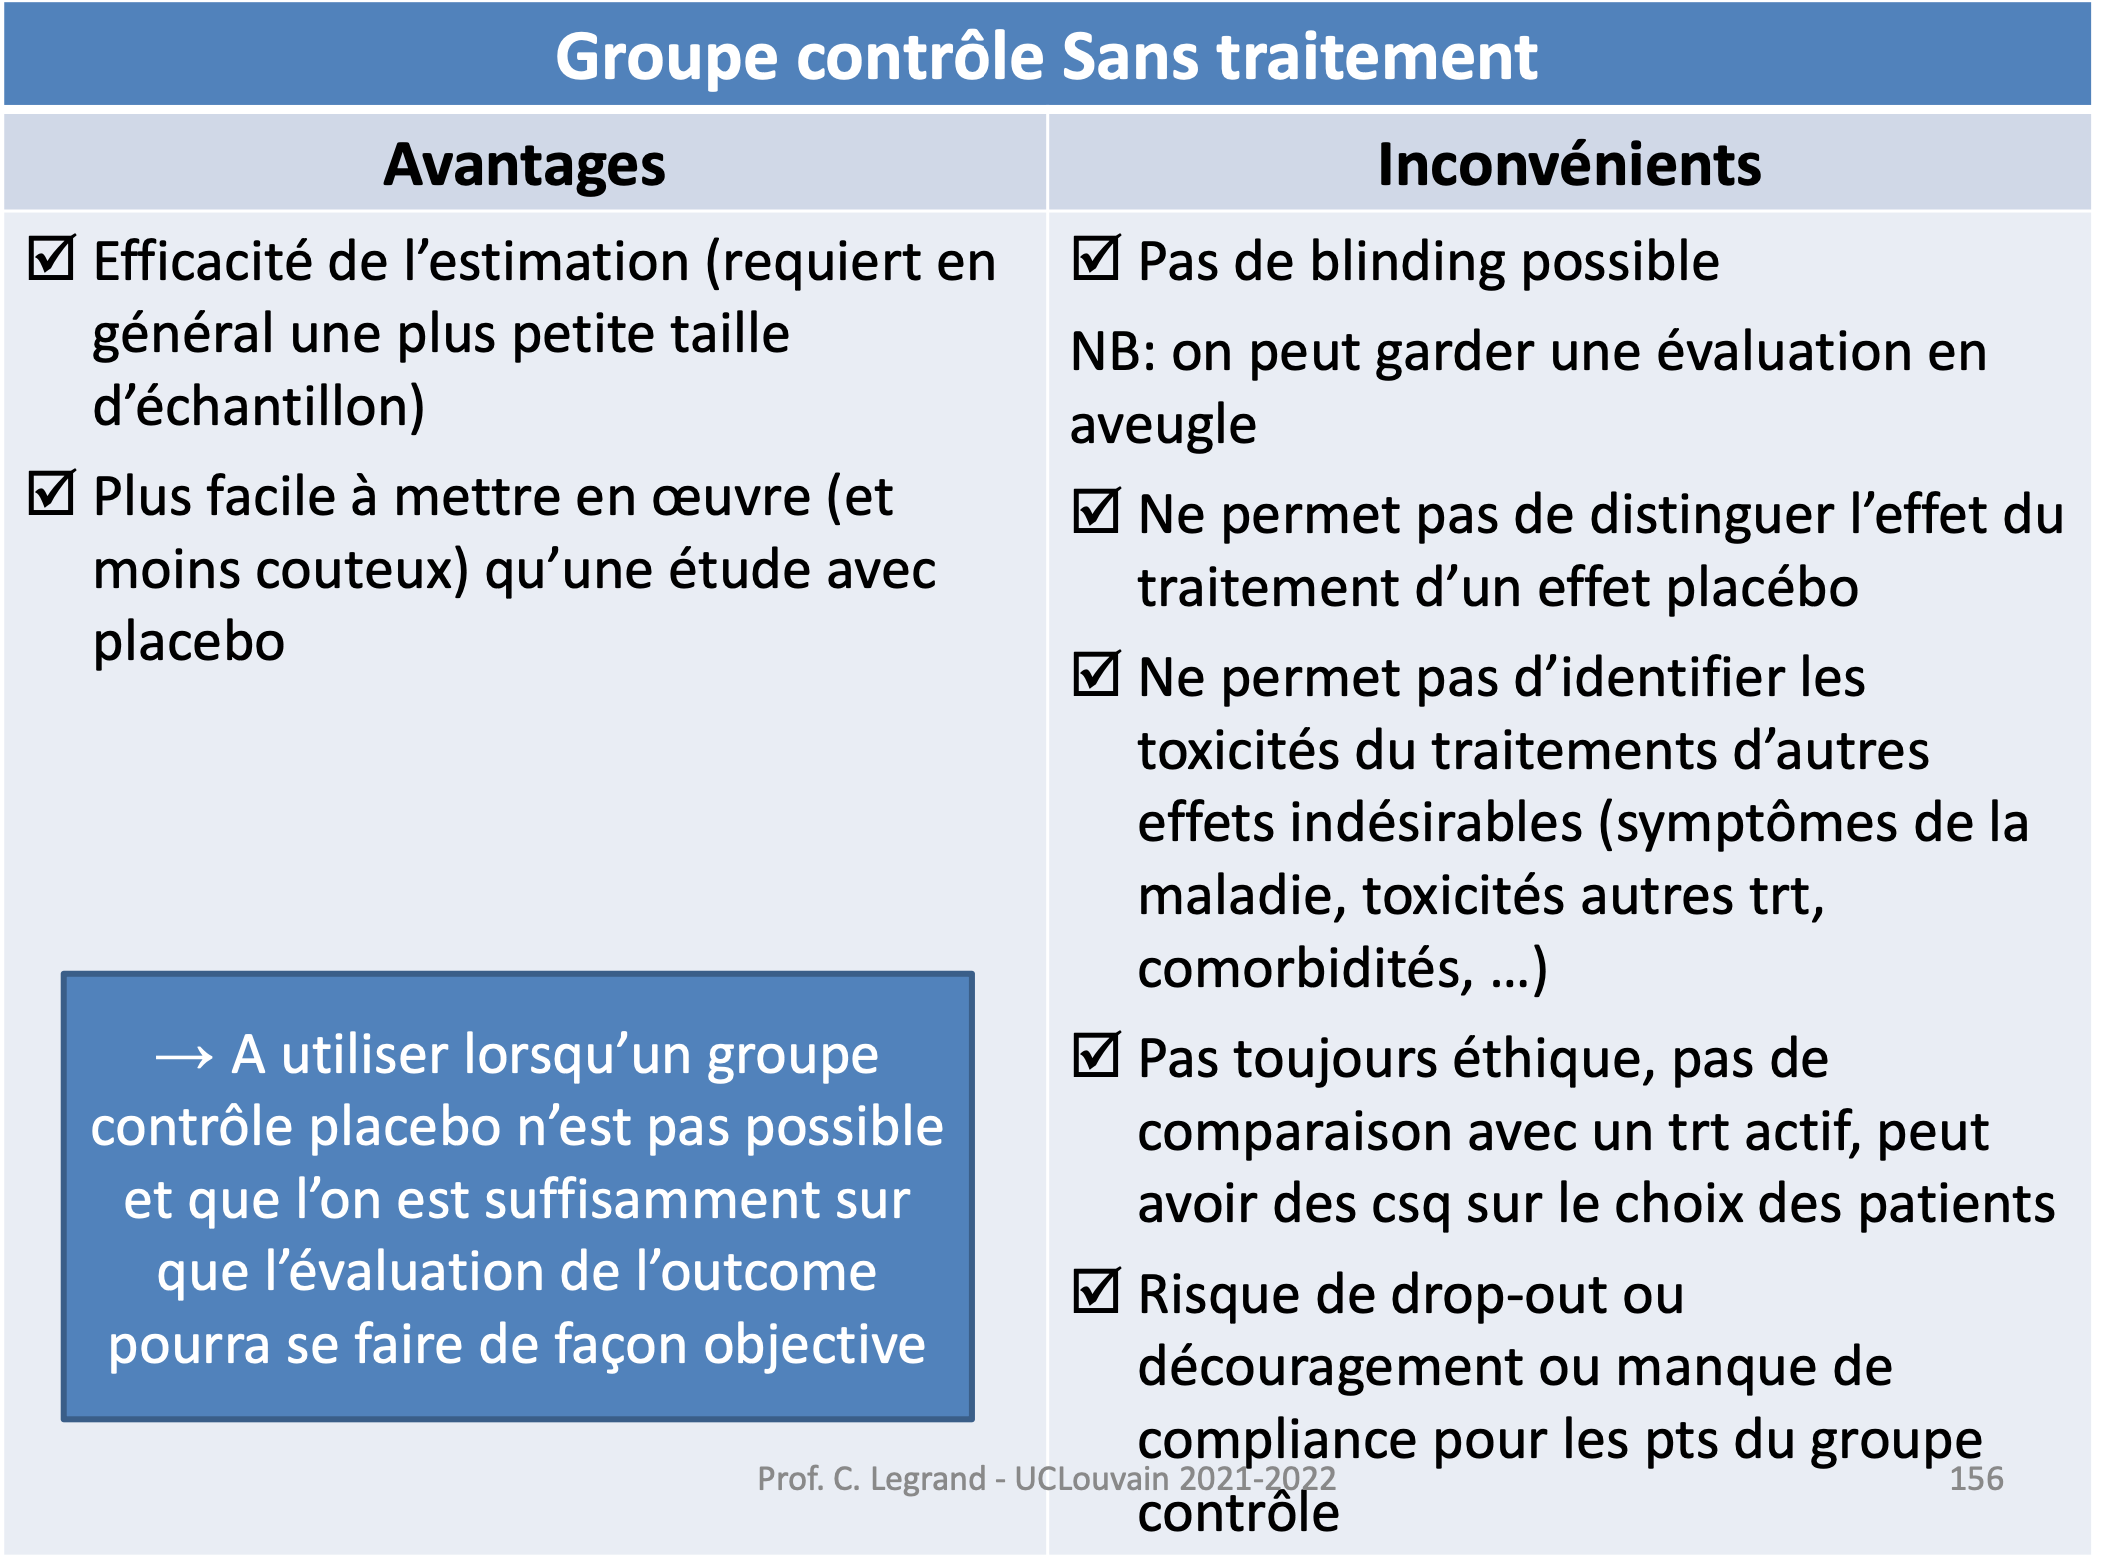
\includegraphics[scale=0.3]{images/no_treatment.png}
    \caption{}
    \label{fig:my_label}
\end{figure}

\section{Objectif de l’essai}

\subsection{Essai de Supériorité ou de Différence}
Le but est de déterminer si le traitement expérimental est plus efficace que le contrôle.

\begin{figure}[H]
    \centering
    
\includegraphics[scale=0.5]{images/essais_diff.png}
    \caption{}
    \label{fig:my_label}
\end{figure}

\textbf{Recommandations}\\

\begin{itemize}
    \item Choisir de faire un test bilatéral ou unilatéral en fonction de l’objectif de l’étude. On recommande en général de faire un test unilatéral uniquement lorsque la différence est d’office dans un sens.
    \item Choisir si le test sera bilatéral ou unilatéral avant d’avoir accès aux données de l’étude.
    \item Lorsque l’on présente une P-valeur, toujours spécifier à quel type de test celle-ci se rapporte.
    \item Toujours vérifier si un test est bilatéral ou unilatéral avant d’interpréter sa p-valeur et interpréter les résultats du test en fonction du type de test.
    \item Ne pas « surinterpréter » une p-valeur non significative
\end{itemize}

\subsection{Essai de Non-infériorité}
Déterminer si le traitement expérimental est "au moins aussi efficace" que le traitement standard, mais une des caractéristiques suivantes :
\begin{itemize}
    \item Moins agressif
    \item Moins toxique
    \item Moins invasif
    \item Moins couteux, plus faisable
\end{itemize}
Ces derniers points doivent être prouvés par \textbf{Endpoints secondaires}!

\begin{figure}[H]
    \centering
    
\includegraphics[scale=0.5]{images/nodiff.png}
    \caption{Hypothèse pour essai de non-infériorité}
    \label{fig:my_label}
\end{figure}

\textbf{Remarques}\\
\begin{itemize}
    \item Il s’agit donc clairement d’un test unilatéral, on verra que ce test est
souvent réalisé via le calcul d’un intervalle de confiance.
\item Si on démontre la non-infériorité, il faut obligatoirement montrer
l’avantage sur un autre endpoint.
\item Démontrer la non-infériorité contre un placebo ou un bras contrôle
non-actif n’a (en général) pas de sens
\end{itemize}


\subsection{Essai d’équivalence}
Déterminer si le traitement expérimental a la même efficacité que le traitement standard (ni moins bon, ni meilleur). Ces tests sont assez rares en recherche clinique et sont surtout utilisé pour les traitements « génériques ».

\begin{figure}[H]
    \centering
    
\includegraphics[scale=0.4]{images/equil.png}
    \caption{Hypothèse essai d'équivalence}
    \label{fig:essaisequi}
\end{figure}

\vspace{0.15cm}
\textbf{\textit{Peut-on conclure à la non-infériorité (ou
l’équivalence) au départ d’un essai clinique
de supériorité non significatif ?}}\\
On ne peut en général pas conclure la non-infériorité /
équivalence d’un essai clinique de supériorité non significatif. OK dans le cas particulier où une marge de non-infériorité $\Delta$ a
été prédéfinie dans le protocole.

\section{Plan d’expérience}

Le design d’un essai clinique de Phase III doit être choisi de façon à ce que l’essai ait un impact maximal sur la pratique clinique. Il doit avoir les caractéristiques suivantes :\\

\begin{itemize}
    \item simple, à grande échelle, multi-centrique (différents hôpitaux)
    \item randomisé (sauf maladie rare)
    \item endpoints approprié ("hard endpoint")
    \item suffisamment de puissance pour détecter une différence petite a modéré, mais cliniquement importante dans l’effet traitement
\end{itemize}


\begin{center}
    \textbf{ On donnera en général la préférence aux essais les plus simples}
\end{center}
Le plus simple il est, plus il sera facile de convaincre les autres des résultats du test.

On a différents designs de plan possibles.

Le premier est le \textbf{design parallèle à 2 groupes}. 
\begin{figure}[H]
    \centering
    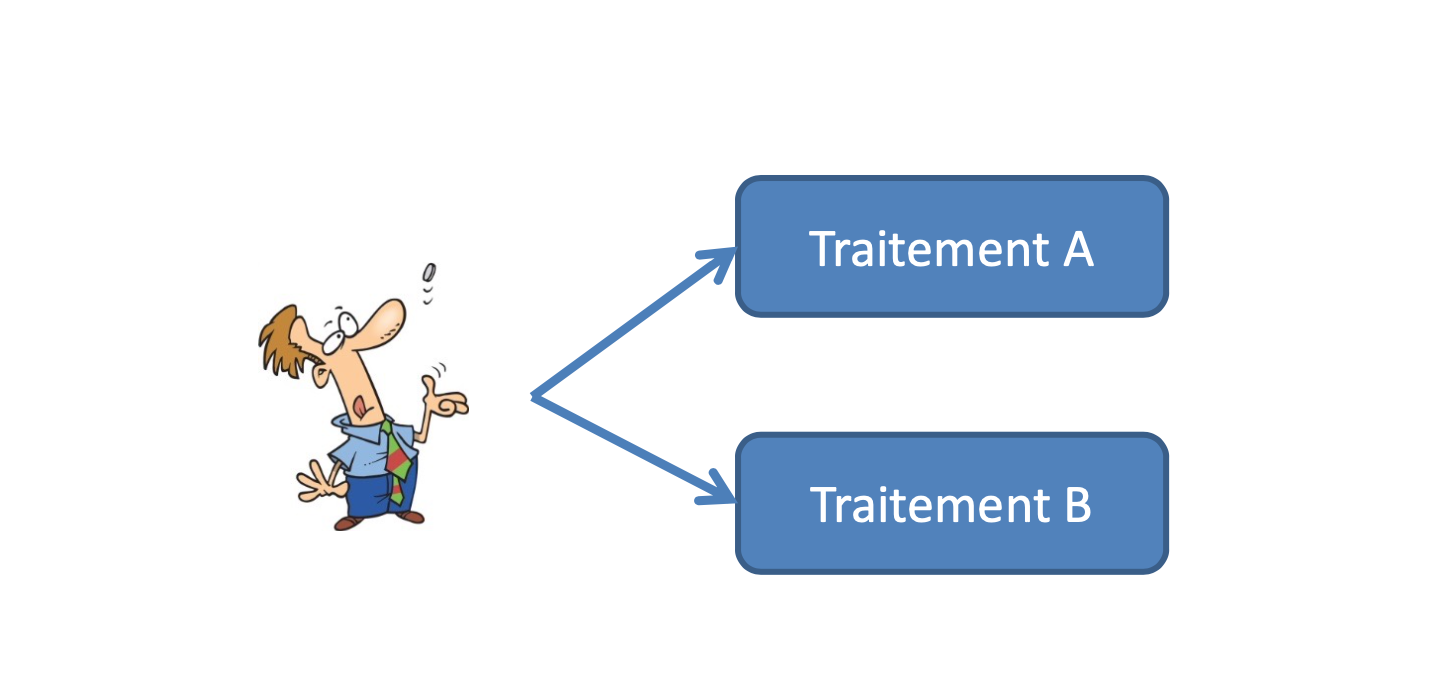
\includegraphics[scale =0.2]{images/2treatments.png}
    \caption{design parallèle à 2 groupes}
    \label{fig:design2}
\end{figure}

Le second est le \textbf{design parallèle à plus de 2 groupes}. Dans le cas de ce design, il est plus difficile de définir les hypothèses pour les tests. 
\begin{figure}[H]
    \centering
    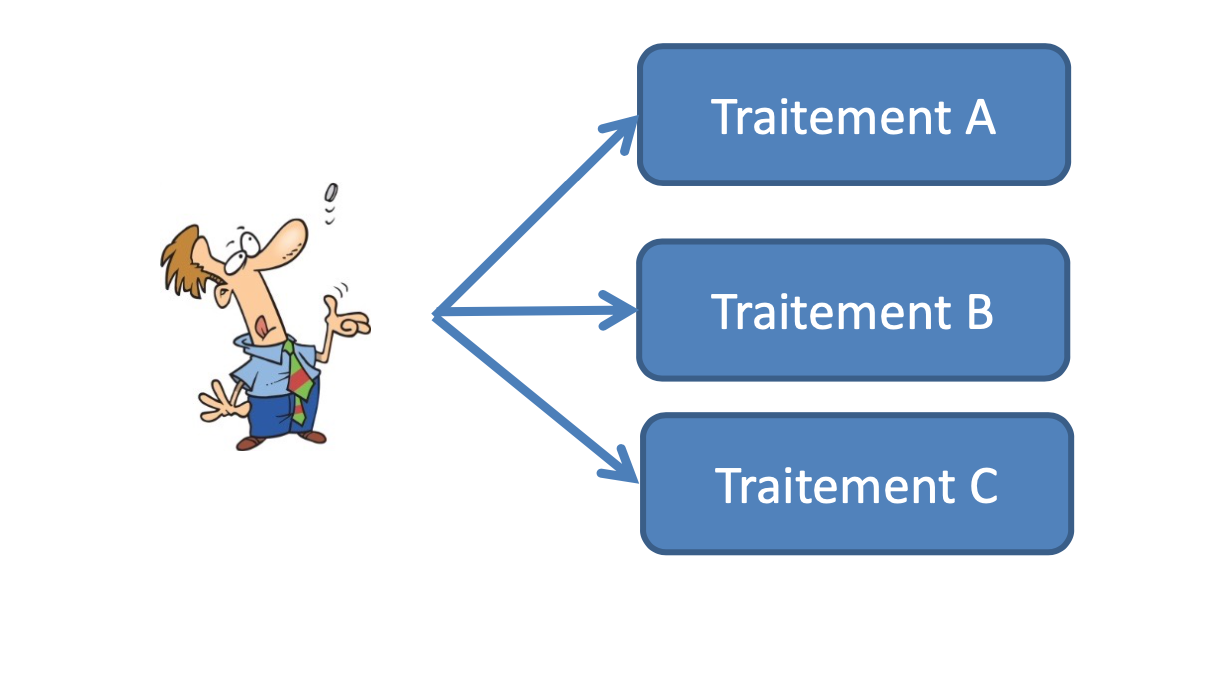
\includegraphics[scale =0.2]{images/more2.png}
    \caption{design parallèle à plus de 2 groupes}
    \label{fig:my_label}
\end{figure}

Il existe des designs plus compliqués où on a en parallèle plusieurs groupes et on réalise en plusieurs étapes les essais.Exemple : MAM (multiple arm) trial.

On a aussi le \textbf{design factoriel 2x2}. Ici, on doit avoir comme hypothèse qu'il n'y a pas d'interaction entre les traitements testés dans les 2 essais.
\begin{figure}[H]
    \centering
    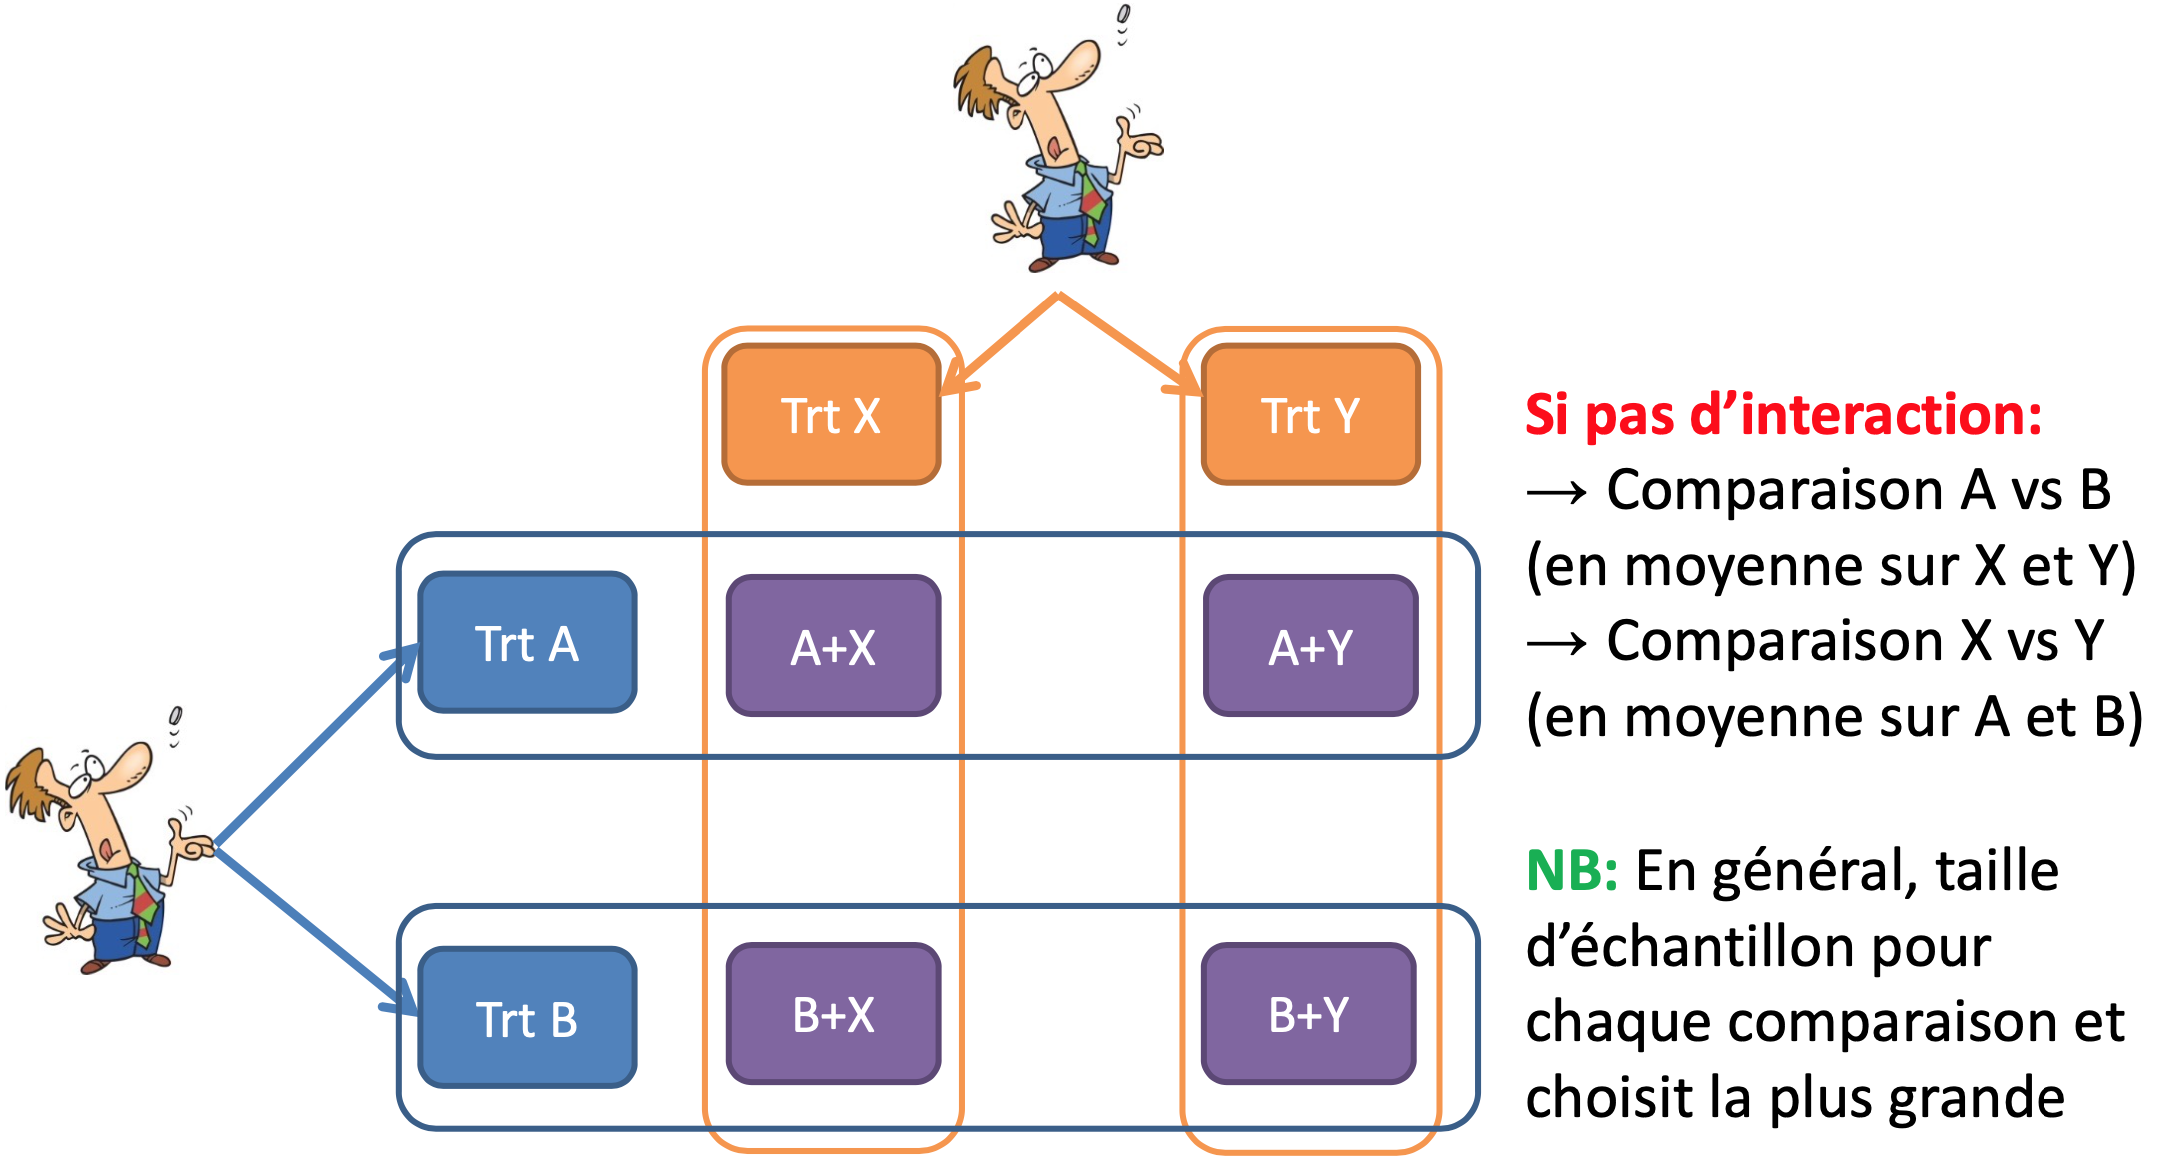
\includegraphics[scale = 0.2]{images/parallel.png}
    \caption{design factoriel 2x2}
    \label{fig:designfactoriel}
\end{figure}

Enfin, on a le \textbf{design cross-over}. Le patient va recevoir tous les traitements, mais dans des ordres différents. Cela a comme effet de diminuer la variabilité, car on fait des comparaisons \textbf{intra-patient}. Le patient est son propre contrôle. Le grand avantage est qu'on a besoin d'un échantillon réduit, mais les techniques de statistiques doivent être adaptées. 
Quelques hypothèses pour ce type de design :
\begin{itemize}
    \item Ordre dans lequel on donne les traitements n'a pas d'importance.
    \item Patients dans le même état avant de commencer chaque période. On n'a pas une dégradation ou une guérison entre les différentes phases.
    \item On travaille sur des endpoints à court terme. 
\end{itemize}


\begin{figure}[H]
    \centering
    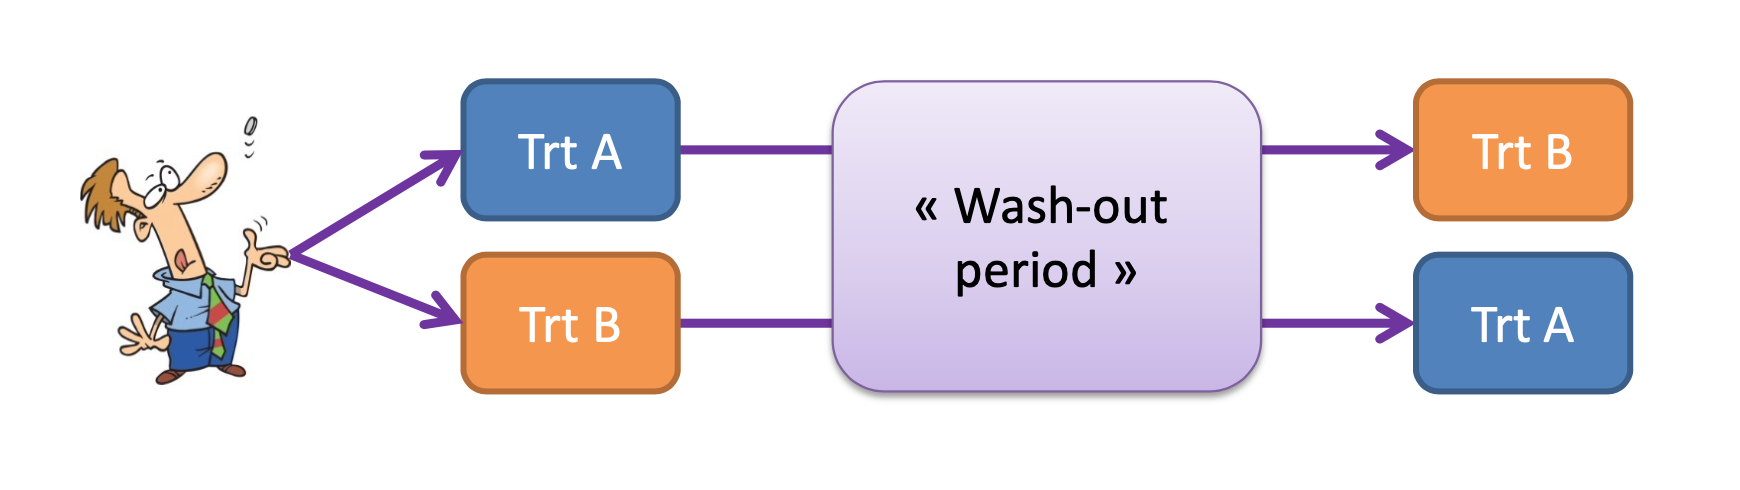
\includegraphics[scale =0.2]{images/overcrossing.png}
    \caption{design cross-over}
    \label{fig:my_label}
\end{figure}



\section{Sélection des patients}
Dernière phase du développement clinique d’un nouveau traitement. \textbf{La définition de la population d’intérêt est cruciale}. On va faire un compromis entre aussi que possible et très restrictif.

\begin{figure}
    \centering
    \includegraphics{}
    \caption{sélections des patients : compromis entre les deux situations}
    \label{fig:my_label}
\end{figure}


\section{Monitoring et IDMC}
La randomisation des patients entre les différents traitements n’est éthiquement acceptable que si le médecin (et de façon générale la communauté scientifique) est en état d’équipoise \footnote{L’équipoise du médecin-chercheur, cet état de réelle incertitude quant aux mérites respectifs de deux traitements à comparer, est, du moins théoriquement — parce qu’impossible dans l’absolu —, l’une des exigences éthiques de l’essai clinique, tout comme l’est l’adoption d’une méthodologie qui respecte les canons de la science.}.\\
Pendant le cours d'un essai clinique, il peut devenir claire que :
\begin{itemize}
    \item soit pour certains/tous les patients un des traitements est meilleur que les autres.
    \item soit que le traitement est trop toxique pour certains/tous les patients.
\end{itemize}

Dans ce cas, on n'est pas dans un état d'équipoise et donc il est nécessaire de stopper l'essai clinique même si cela entraine des conséquences négatives.

C'est pour cela qu'on fait appel à des gens extérieurs pour cette étape.







\chapter{Phase III - randomisation}
c'est la partie que la prof n'aime pas.\\

Affectation des différents traitements aux unités expérimentales de manière aléatoire.\\

\begin{itemize}
    \item Comparaison non biaisée des traitements [selection bias]
    \item Si grand nombre d’unités expérimentales : variables concomitantes
distribuée également entre les groupes trt [confondant facteurs]
    \item Base de l’inférence statistique
\end{itemize}

Principe de randomisation :
\begin{itemize}
    \item chaque patient à la même chance de recevoir chacun des traitements étudiés
    \item l’assignement d’un patient à un groupe traitement n’influence pas le choix du traitement des autres patients
    \item on ne sait pas à l’avance quel traitement chacun des patients va recevoir
\end{itemize}
\section{Randomisation simple}
Assignation des patients au traitement expérimental (EXP) ou
au traitement contrôle (CRT) sans raffinement.\\

Si la taille d’échantillon est petite, la randomisation simple n’est pas sans risque et peut quand même conduire à un facteur confondant n’étant pas équitablement réparti dans les deux groupes.


\section{Randomisation stratifiée}
La randomisation simple est réalisée séparément dans chacune des strates de la population définie par le facteur confondant.\\

La randomisation simple est réalisée séparément dans chacune des strates de la population définie par le facteur confondant.\\

Si la taille d’échantillon est petite, la randomisation simple et la randomisation stratifiée peut conduire à un nombre différent de patients dans chacun des groupes traitements.

\section{Randomisation restreinte ou par bloc}
La randomisation restreinte ou par bloc permet de limiter le déséquilibre dans l’assignement des groupes traitements. On choisit au préalable une taille n de bloc et on s’assure qu’un équilibre traitement est atteint après que n patients soient entrés dans l’étude.\\

 
Viole les principes de base de la randomisation, et notamment il devient possible de deviner à l’avance le traitement pour certains patients.


\section{Randomisation par minimisation}

Dans la randomisation par minimisation, la probabilité pour chaque patient d’être assigné à un bras ou un autre est modifiée de façon à favoriser le bras qui va réduire l’imbalance.\\

 
Viole les principes de base de la randomisation, mais moins que la randomisation par bloc ; et notamment garde un caractère aléatoire pour tous les patients.




\chapter{Phase III - analyse}

Différents types d'endpoint sont possibles :
\begin{enumerate}
    \item Endpoint continu
    \item Endpoint discret
    \item Endpoint de survie
\end{enumerate}

\section{Endpoint continu}
Pour chaque patient, on mesure un endpoint continu dont on va en général supposer qu’il suit une distribution approximativement normale. Par exemple, le Taux de cholestérol, Valeur de la pression artérielle, etc.\\

Si on peut supposer que notre endpoint suit une distribution normale, on va en général s’intéresser à la moyenne de cette distribution pour chaque bras de traitement

\subsection{Cas de deux groupes de traitements}

on considère deux groupes de traitement.
\begin{figure}[H]
    \centering
    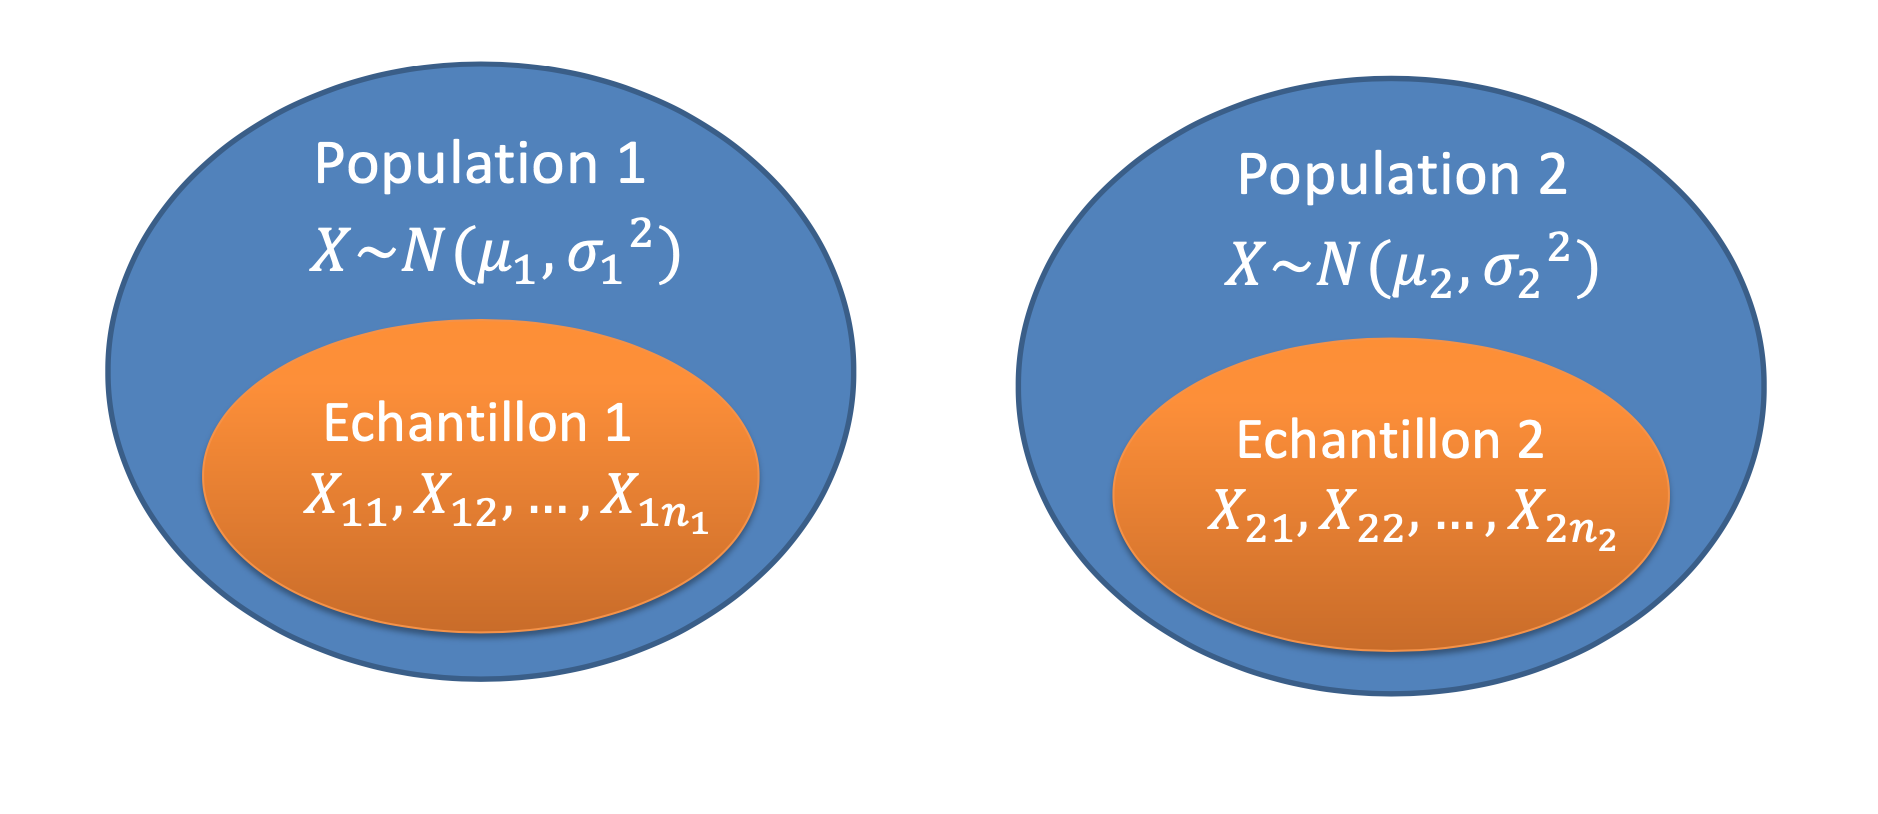
\includegraphics[scale = 0.5]{images/2groupescontinu.png}
    \caption{deux groupes de traitement}
    \label{fig:my_label}
\end{figure}




Test t de Student pour comparer deux moyennes :
\begin{figure}[H]
    \centering
    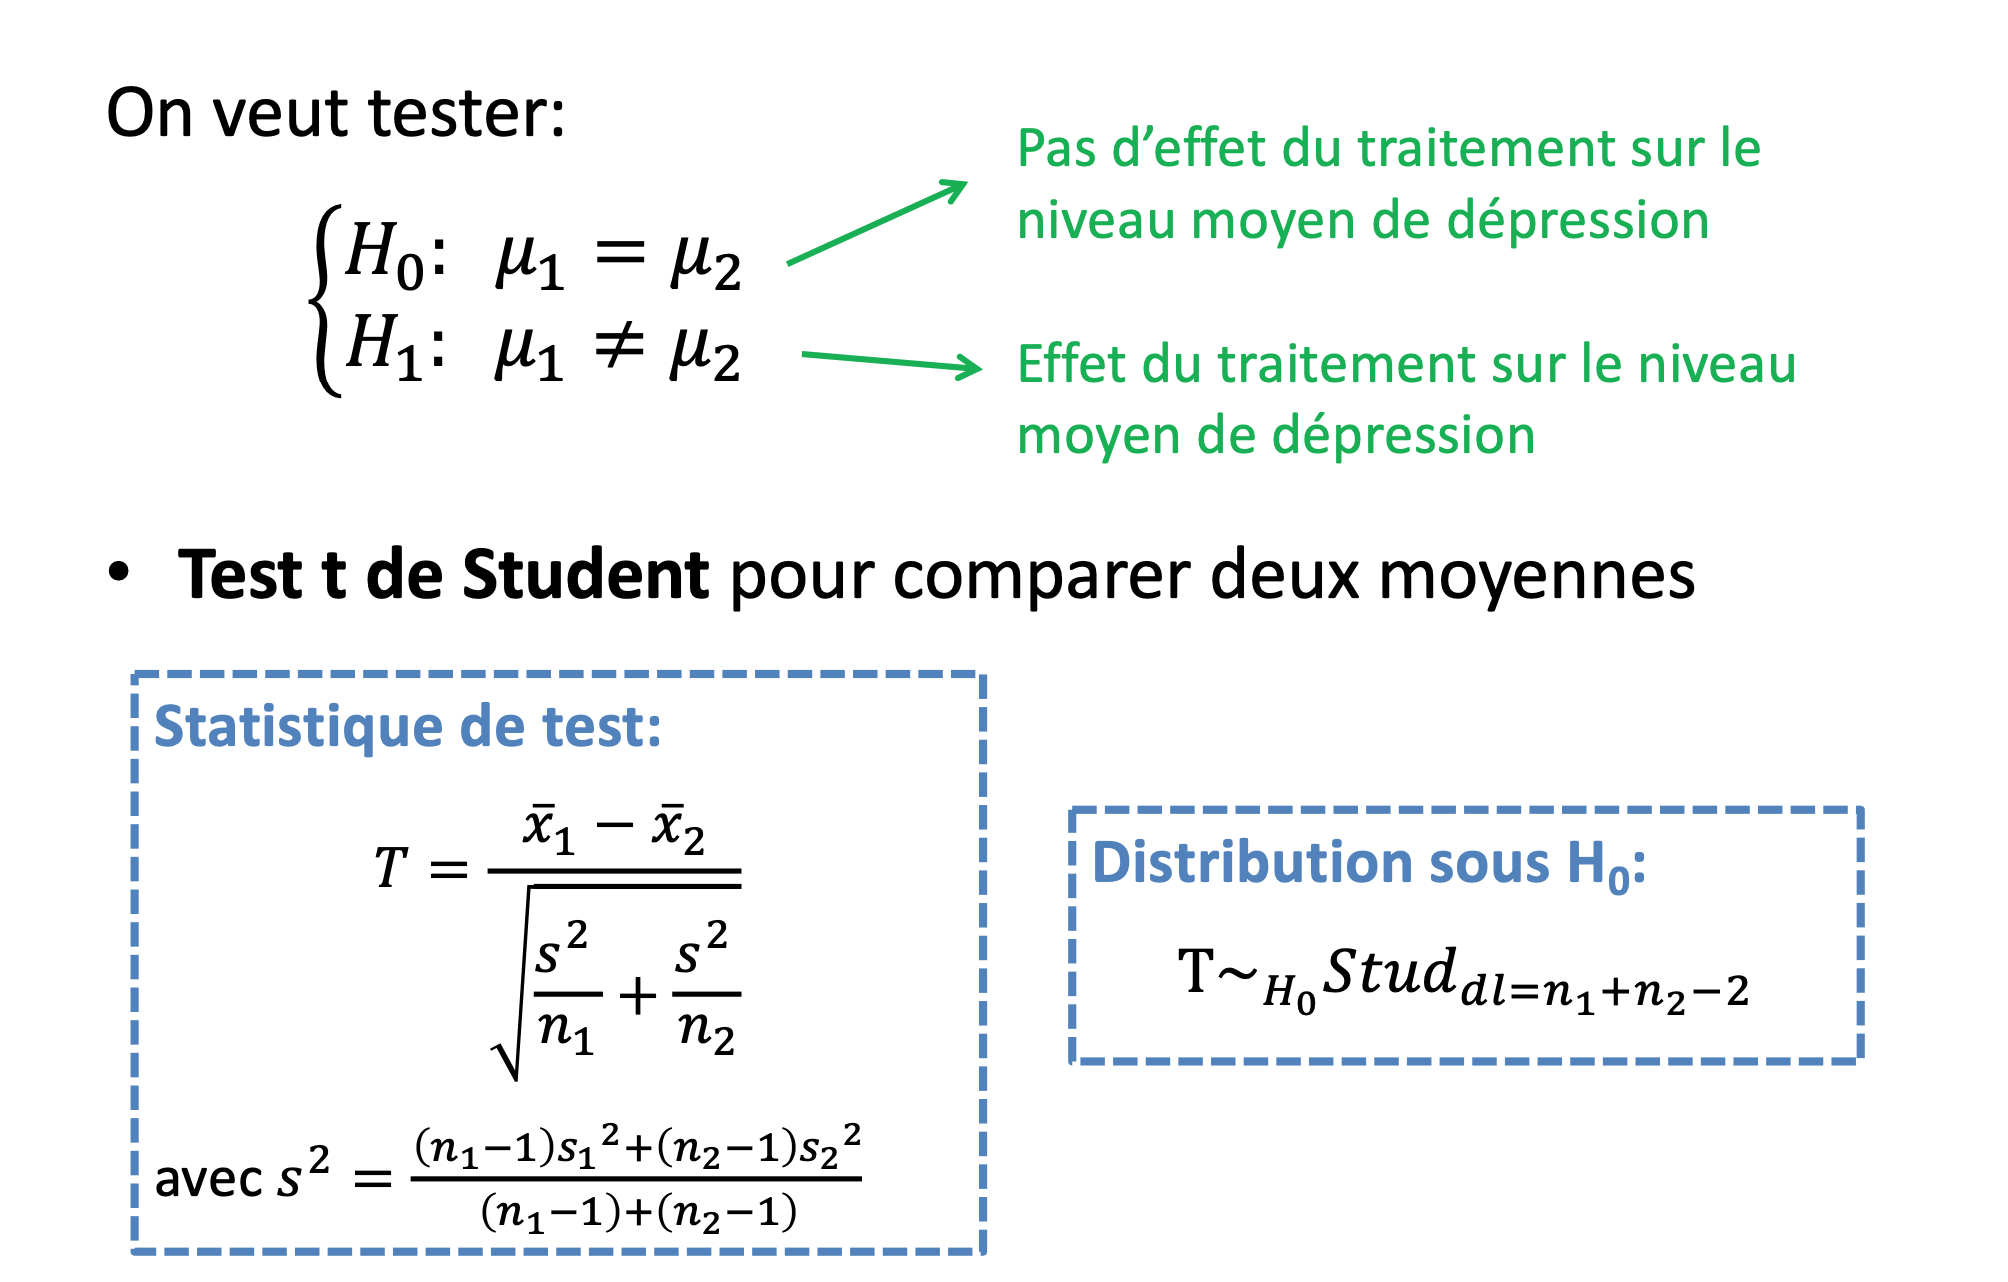
\includegraphics[scale=0.3]{images/student.png}
    \caption{Test t de Student pour comparer deux moyennes}
    \label{fig:my_label}
\end{figure}


\textbf{Remarques}
\begin{enumerate}
    \item \textbf{Conditions d’applications du test t de Student:}
    \begin{itemize}
        \item X est une variable continue de distribution (approximativement) normale, et de même variance dans les deux sous-populations considérées
        \item Les deux échantillons(aléatoires) sont indépendants
    \end{itemize}
    \item Si on ne peut pas supposer $\sigma_{1}^{2}=\sigma_{2}^{2}$, il existe une autre formulation de ce test
    
    \item Test de Welch: dans le cas où on ne peut supposer $\sigma_{1}^{2}=\sigma_{2}^{2}$, une meilleure approximation de la distribution sous H0 est donnée dans la figure \ref{fig:welch}
    \item Si on ne peut pas supposer la normalité approximative :
    \begin{itemize}
        \item On peut essayer de transformer la variable X, par exemple en considérant log(X), pour améliorer l’approximation normale
        \item On peut réaliser un test non paramétrique : Mann-Whitney-Wilcoxon U-test


    \end{itemize}
\end{enumerate}

\begin{figure}[H]
    \centering
    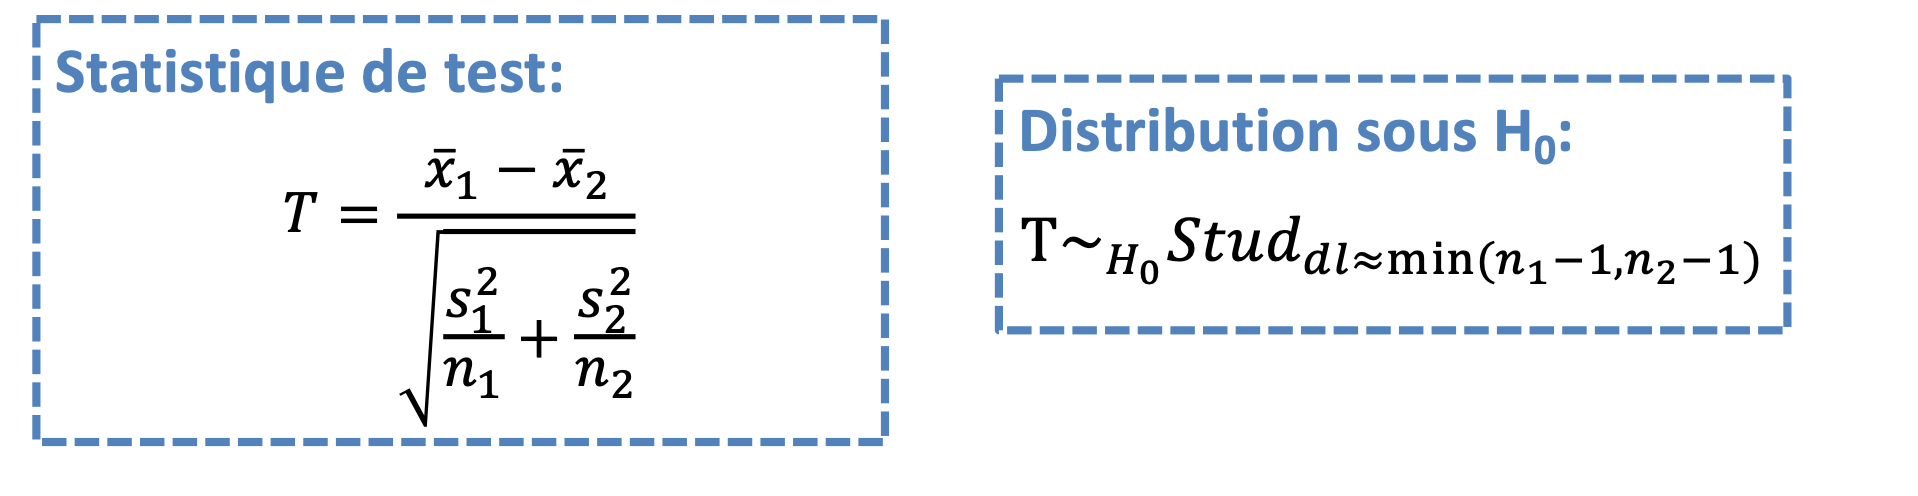
\includegraphics[scale = 0.5]{images/studentbis.png}
    \caption{Test t de Student pour comparer deux moyennes si $\sigma_{1}^{2} \neq \sigma_{2}^{2}$}
    \label{fig:studbis}
\end{figure}

\begin{figure}[H]
    \centering
    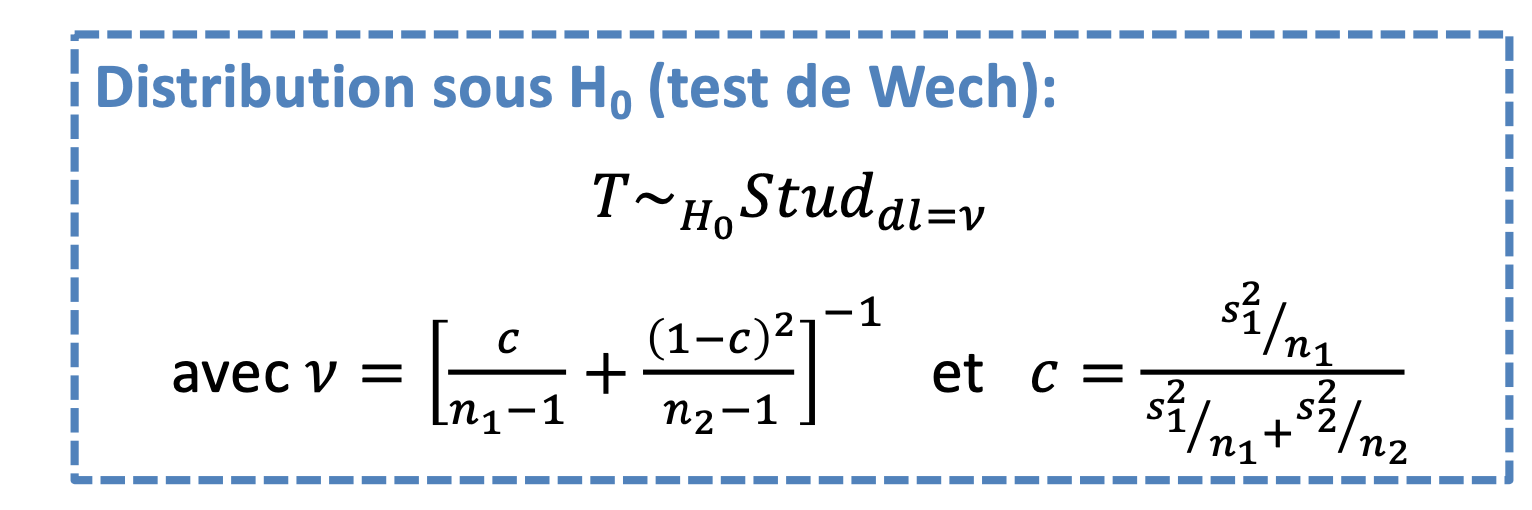
\includegraphics[scale = 0.5]{images/Welch.png}
    \caption{Test de Welch}
    \label{fig:welch}
\end{figure}

\subsubsection{Cas des données pairées}
Chaque observation du groupe 1 est liée à une (et une seule)
observation du groupe 2. On va faire un Test T pairé: pour chaque paire (i=1, ..., N) on considère la différence $d$

\begin{figure}[H]
    \centering
    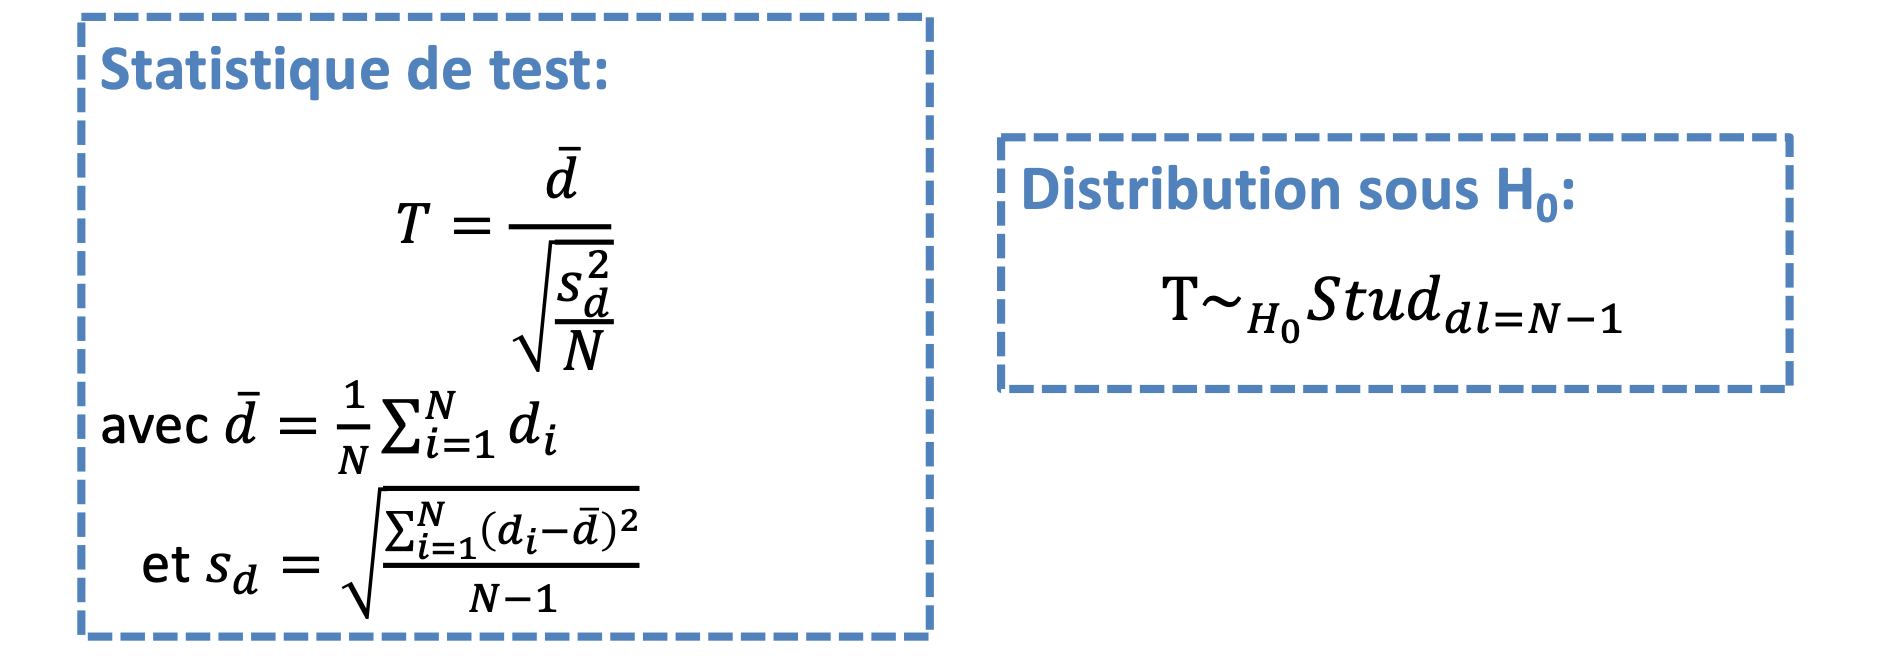
\includegraphics[scale = 0.5]{images/testTpaire.png}
    \caption{Test T pairé}
    \label{fig:my_label}
\end{figure}

\subsubsection{Estimation de l'effet traitement}
Pour un endpoint continu (approximativement normal), l’effet du traitement est typiquement résumé par l’estimation de la différence des moyennes $\mu_{1}-\mu_{2}$  et son intervalle de confiance à $1 − \alpha \%$
\subsection{Cas de plus de 2 groupes de traitement}
\textbf{Idée}: faire toutes les comparaisons deux à deux.\\ 

\textbf{MAIS}: le nombre de tests augmentent rapidement.
$$\tilde{n} = \frac{k*(k+1)}{2}$$

Il y a deux façons de définir l’erreur de type I dans le contexte de comparaisons multiples, soit Individuel (erreur de type I pour chaque test réalisé) ou Global (probabilité de faire au moins une erreur de
type I à un des tests [Family error rate])

Le risque global d’erreur de type I augmente (très rapidement) avec le nombre de comparaisons\\

$$\alpha_{G}=1-(1-\alpha)^{n_{k}}$$

\begin{figure}[H]
    \centering
    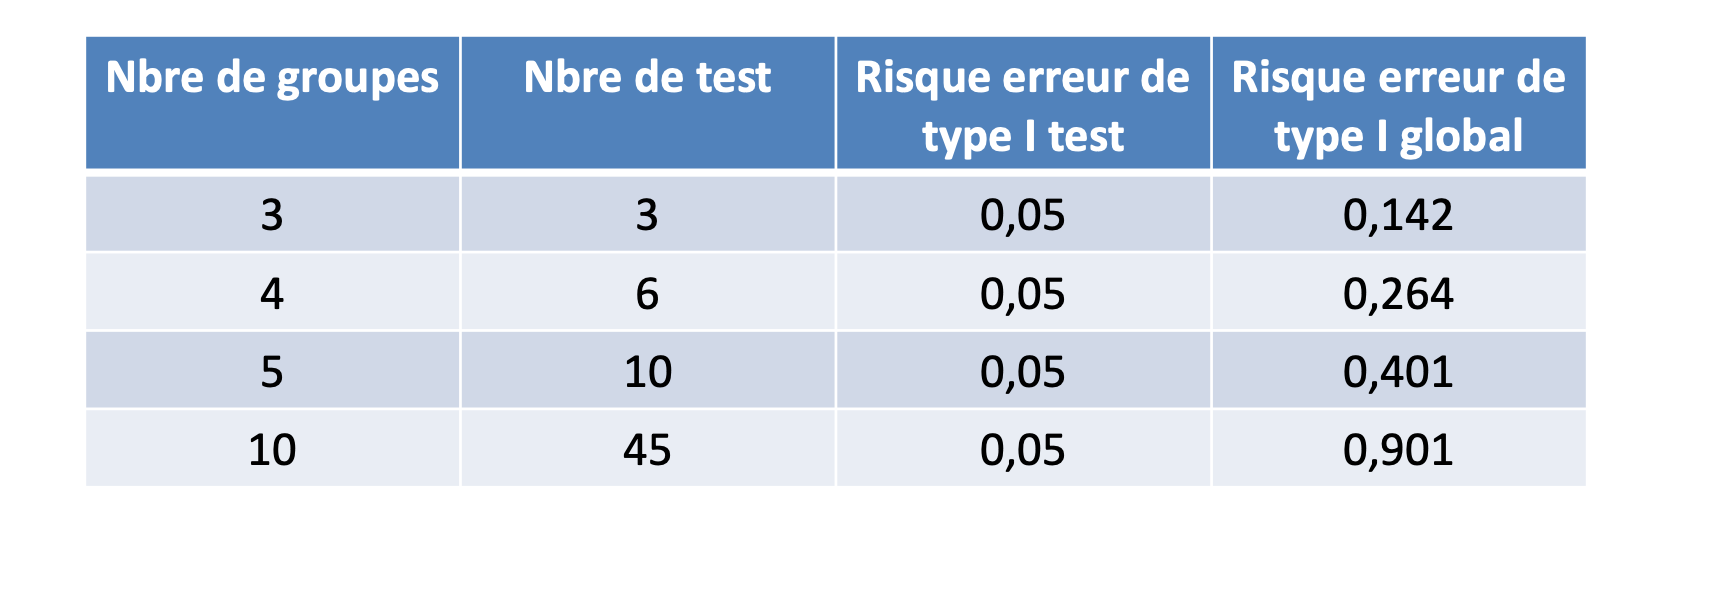
\includegraphics[scale = 0.5]{images/erreurglobal.png}
    \caption{augmentation erreur globale de type I}
    \label{fig:my_label}
\end{figure}

\begin{center}
    Donc on a des problèmes de multiplicité des tests
\end{center}

\textbf{Solutions}

\begin{figure}[H]
    \centering
    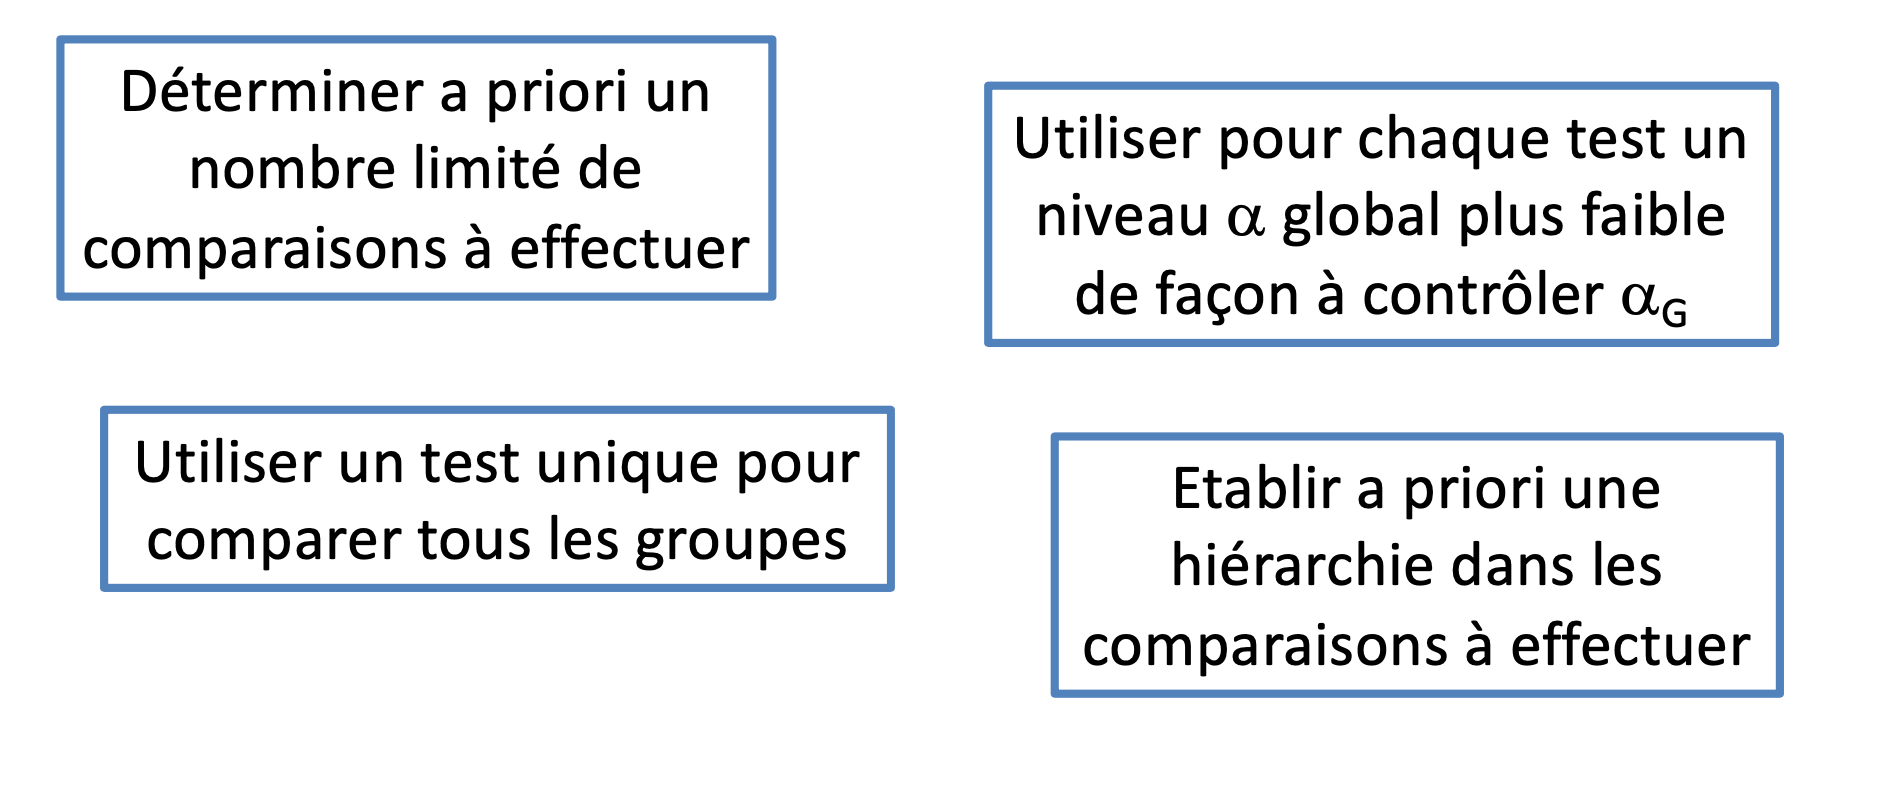
\includegraphics[scale = 0.5]{images/problememultitest.png}
    \caption{Solutions}
    \label{fig:my_label}
\end{figure}

\subsubsection{Utiliser pour chaque test un niveau a global plus faible de façon à contrôler $\alpha_{G}$:procédure de Bonferroni}
$$\tilde{\alpha}= \frac{\alpha}{\tilde{n_{k}}} \Rightarrow \alpha_{G}=1-(1-\tilde{\alpha})^{n_{k}} < \alpha$$

\subsubsection{Utiliser un test unique pour comparer tous les groupes :ANOVA}
\begin{figure}[H]
    \centering
    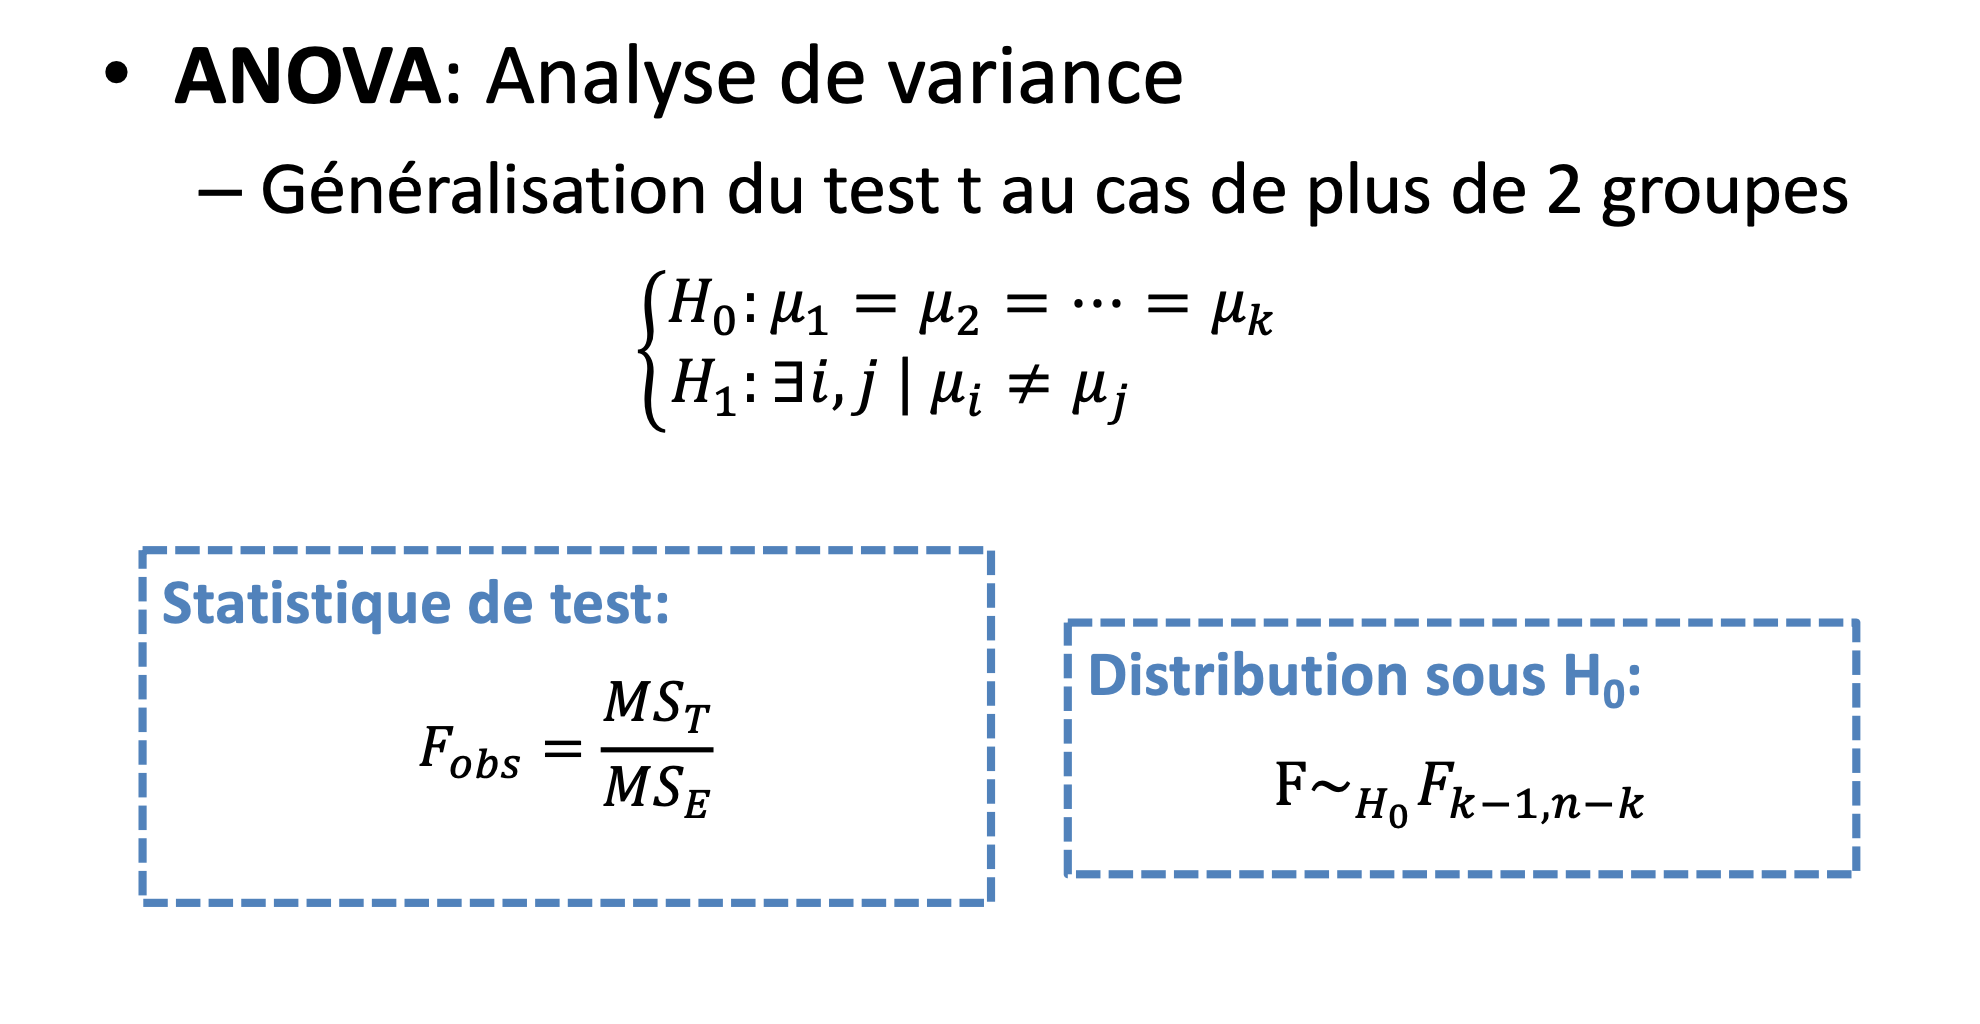
\includegraphics[scale=0.5]{images/anova.png}
    \caption{Test Anova}
    \label{fig:anova}
\end{figure}

\textbf{Remarques}
\begin{enumerate}
    \item Conditions d’applications du test F d’ANOVA:
    \begin{itemize}
        \item X est une variable continue de distribution (approximativement) normale, et de même variance dans toutes les sous-populations considérées
        \item Les observations sont indépendants
    \end{itemize}
    \item On présente souvent les résultats sous la forme d’une table d’ANOVA
    \item Si RHO, il faut encore déterminer quels sont les groupes qui ont des moyennes différentes ! Il faut alors calculer les intervalles de confiance pour les différences de moyennes deux à deux.
\end{enumerate}

Pour résoudre le problème de multiplicité, on plusieurs possibilités :
\begin{itemize}
    \item Méthode LSD de Fisher
    \item Méthode de Tukey-Kramer
    \item Méthode de Dunnett
    \item ...
\end{itemize}

\begin{figure}[H]
    \centering
    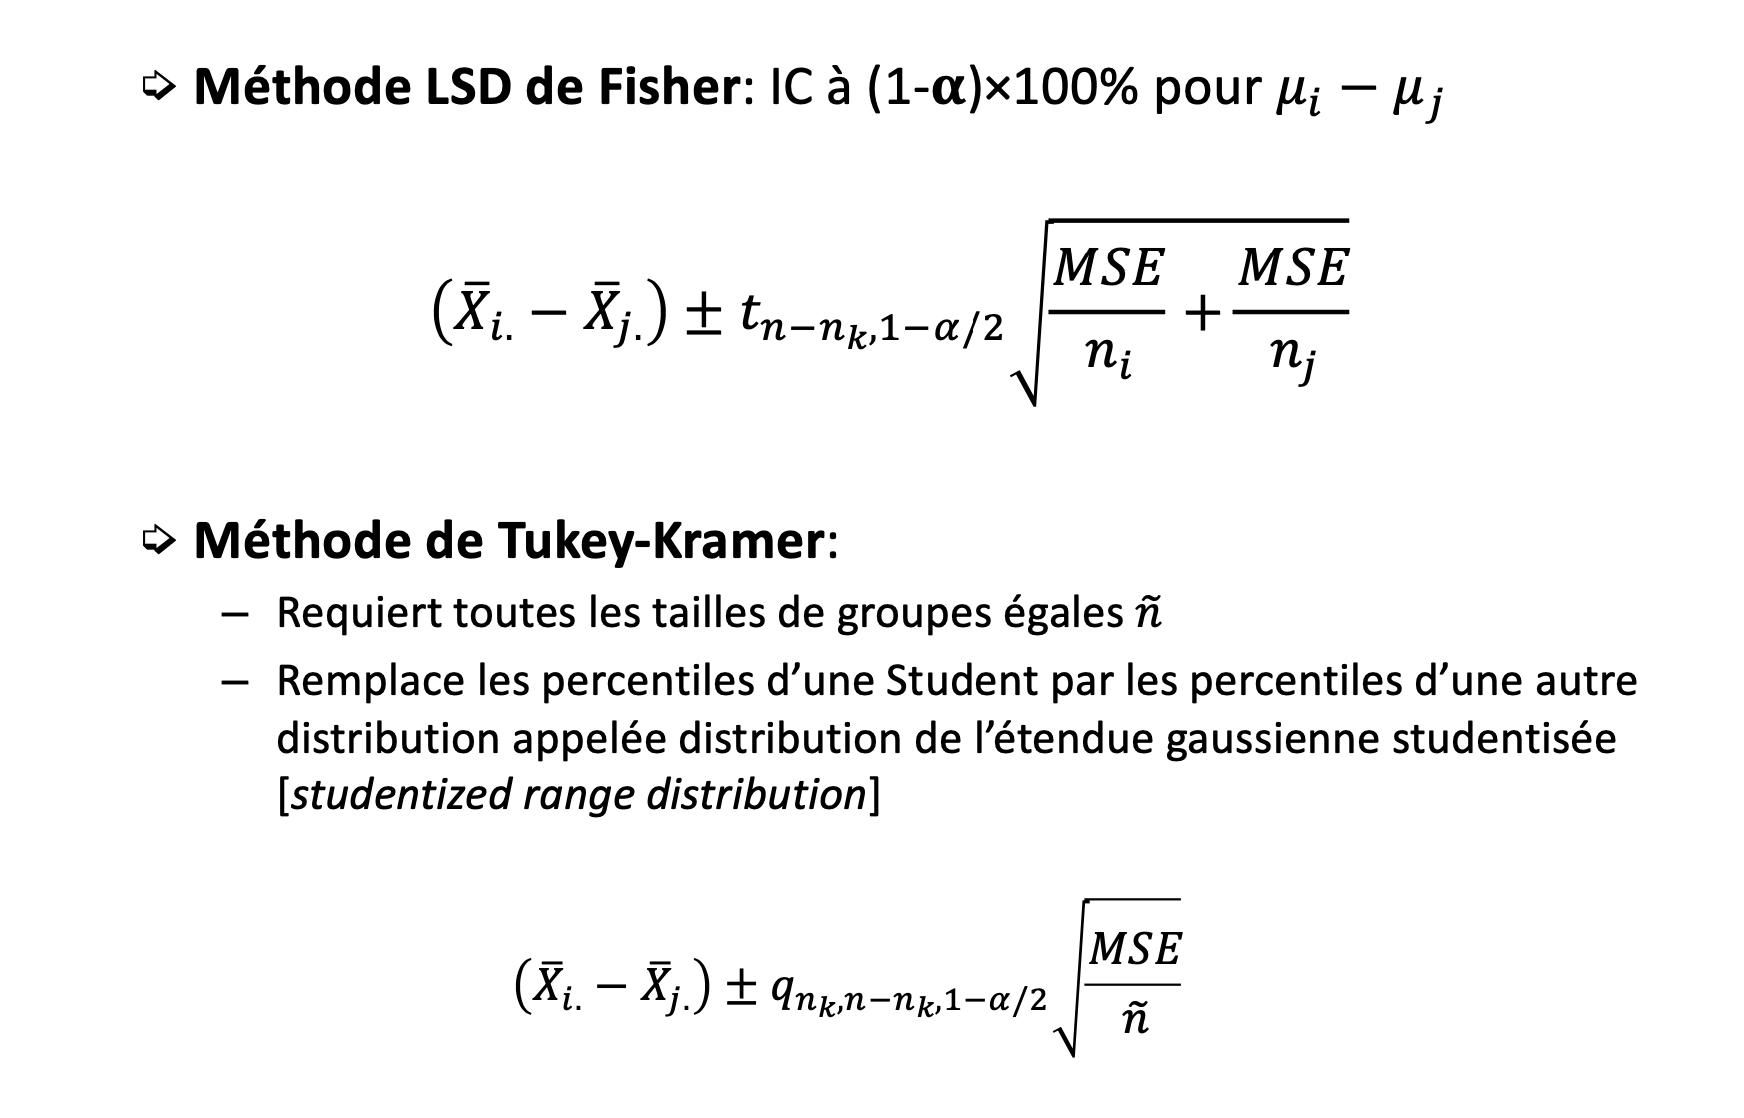
\includegraphics[scale=0.4]{images/LSD_Tukey.png}
    \caption{Méthode de LSD de Fisher et de Tukey-Kramer}
    \label{fig:my_label}
\end{figure}

\begin{figure}[H]
    \centering
    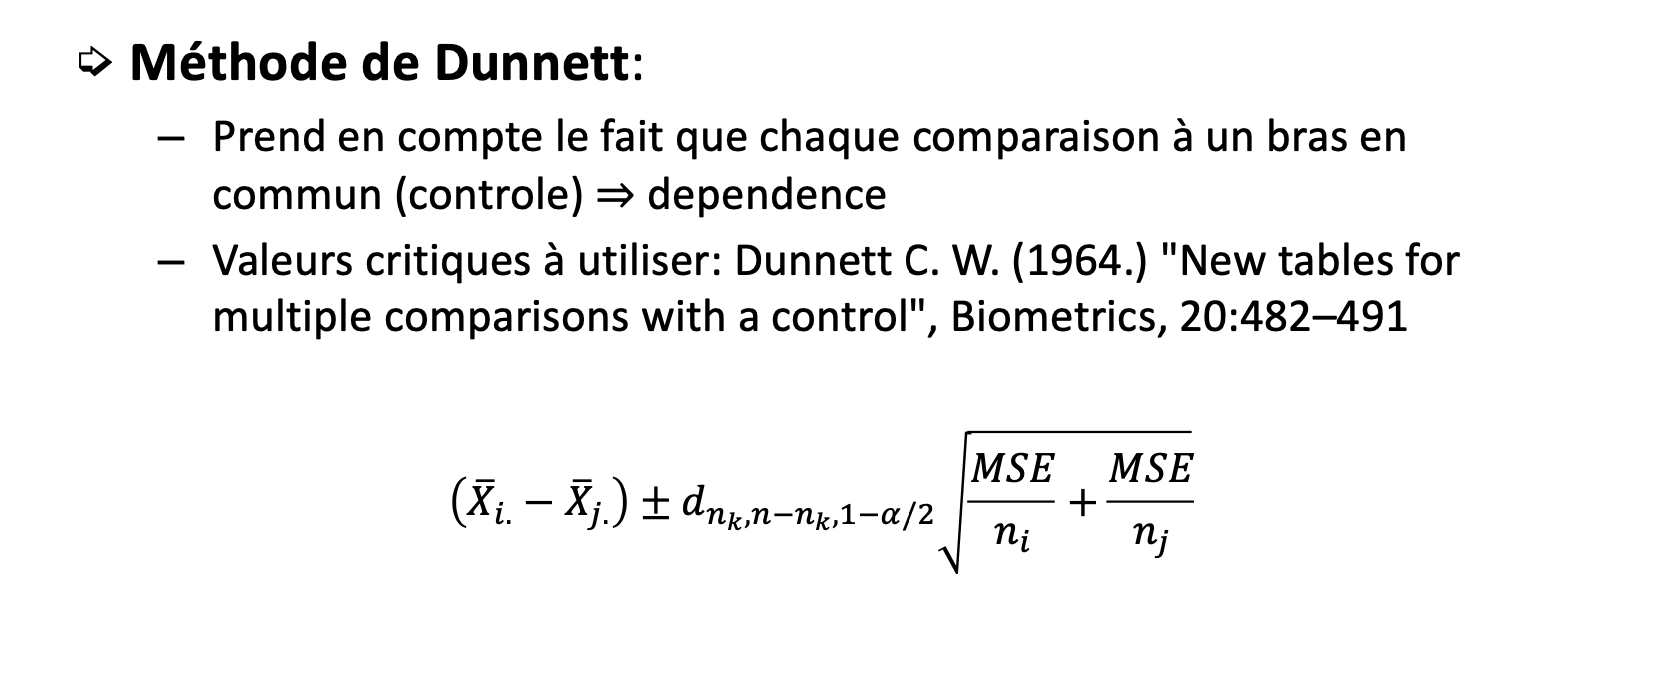
\includegraphics[scale=0.4]{images/Dunnett.png}
    \caption{Méthode de LSD de Dunnett}
    \label{fig:my_label}
\end{figure}


\subsection{Régression linéaire multiple}
On décrit l’association (linéaire) entre Une variable Y (= réponse) continue et plusieurs variables X explicatives.

\begin{figure}[H]
    \centering
    
\includegraphics[scale = 0.5]{images/regressionlineaire.png}
    \caption{formule régression linéaire}
    \label{fig:my_label}
\end{figure}
On trouve les valeurs de  soit par le critère des moindres carrées soit par la méthode du maximum de vraisemblance.\\

On peut interpréter $\beta_k$ comme le changement moyen de la valeur de Y quand $X_{k}$ augmente d’une unité (les valeurs de toutes les autres variables étant fixée).

\section{Endpoint binaire}
Pour chaque patient, l’endpoint binaire se mesure comme étant : Succès ou Échec. 

\subsection{Cas de deux groupes de traitements}

\begin{figure}[H]
    \centering
    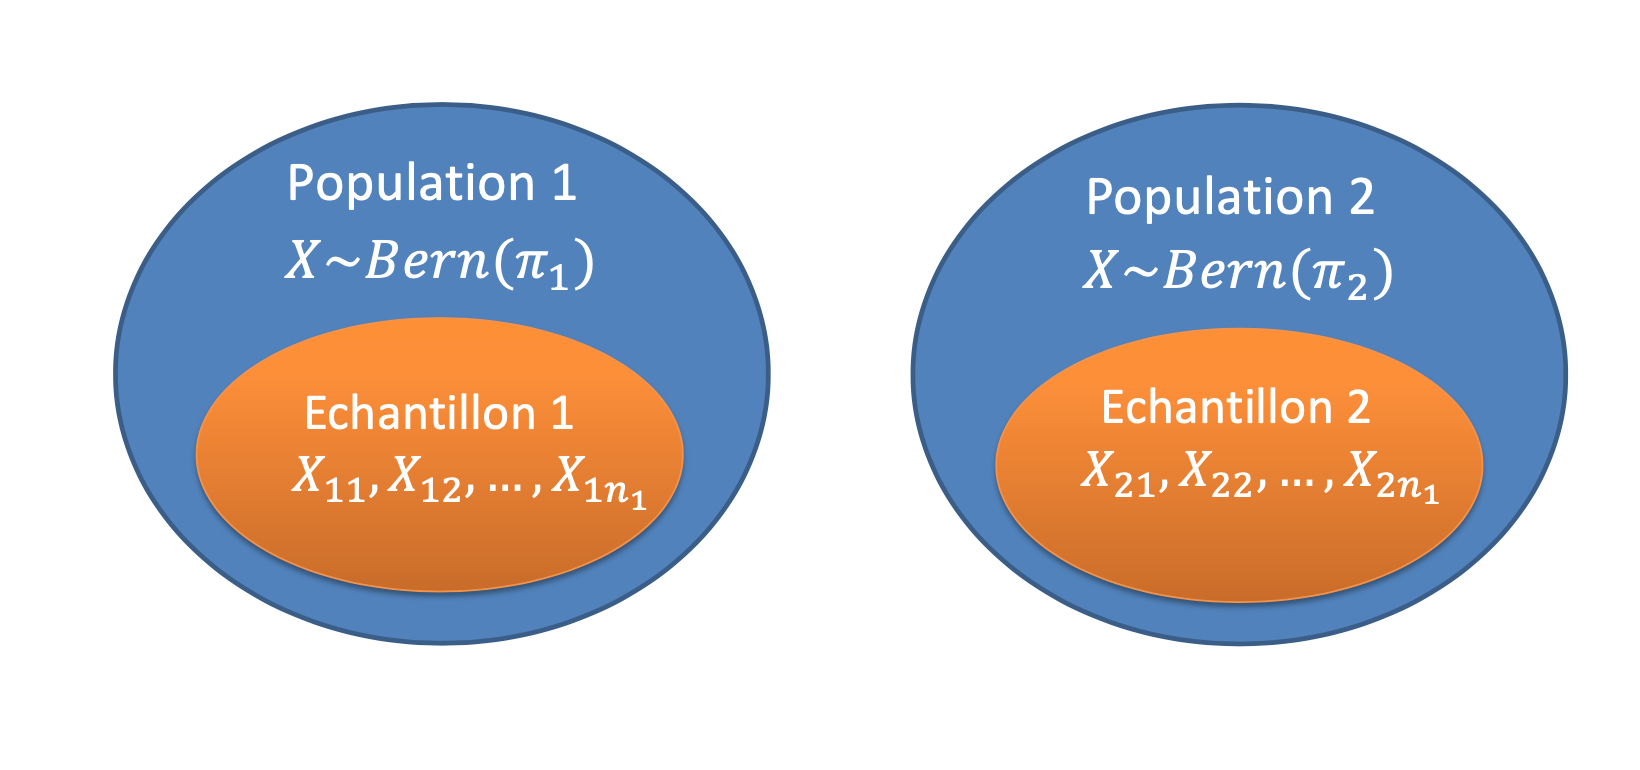
\includegraphics[scale = 0.5]{images/deuxgroupesbinaires.png}
    \caption{Cas de deux groupes de traitements}
    \label{fig:my_label}
\end{figure}

\subsubsection{Test Z pour comparer deux probabilités}

\begin{figure}[H]
    \centering
    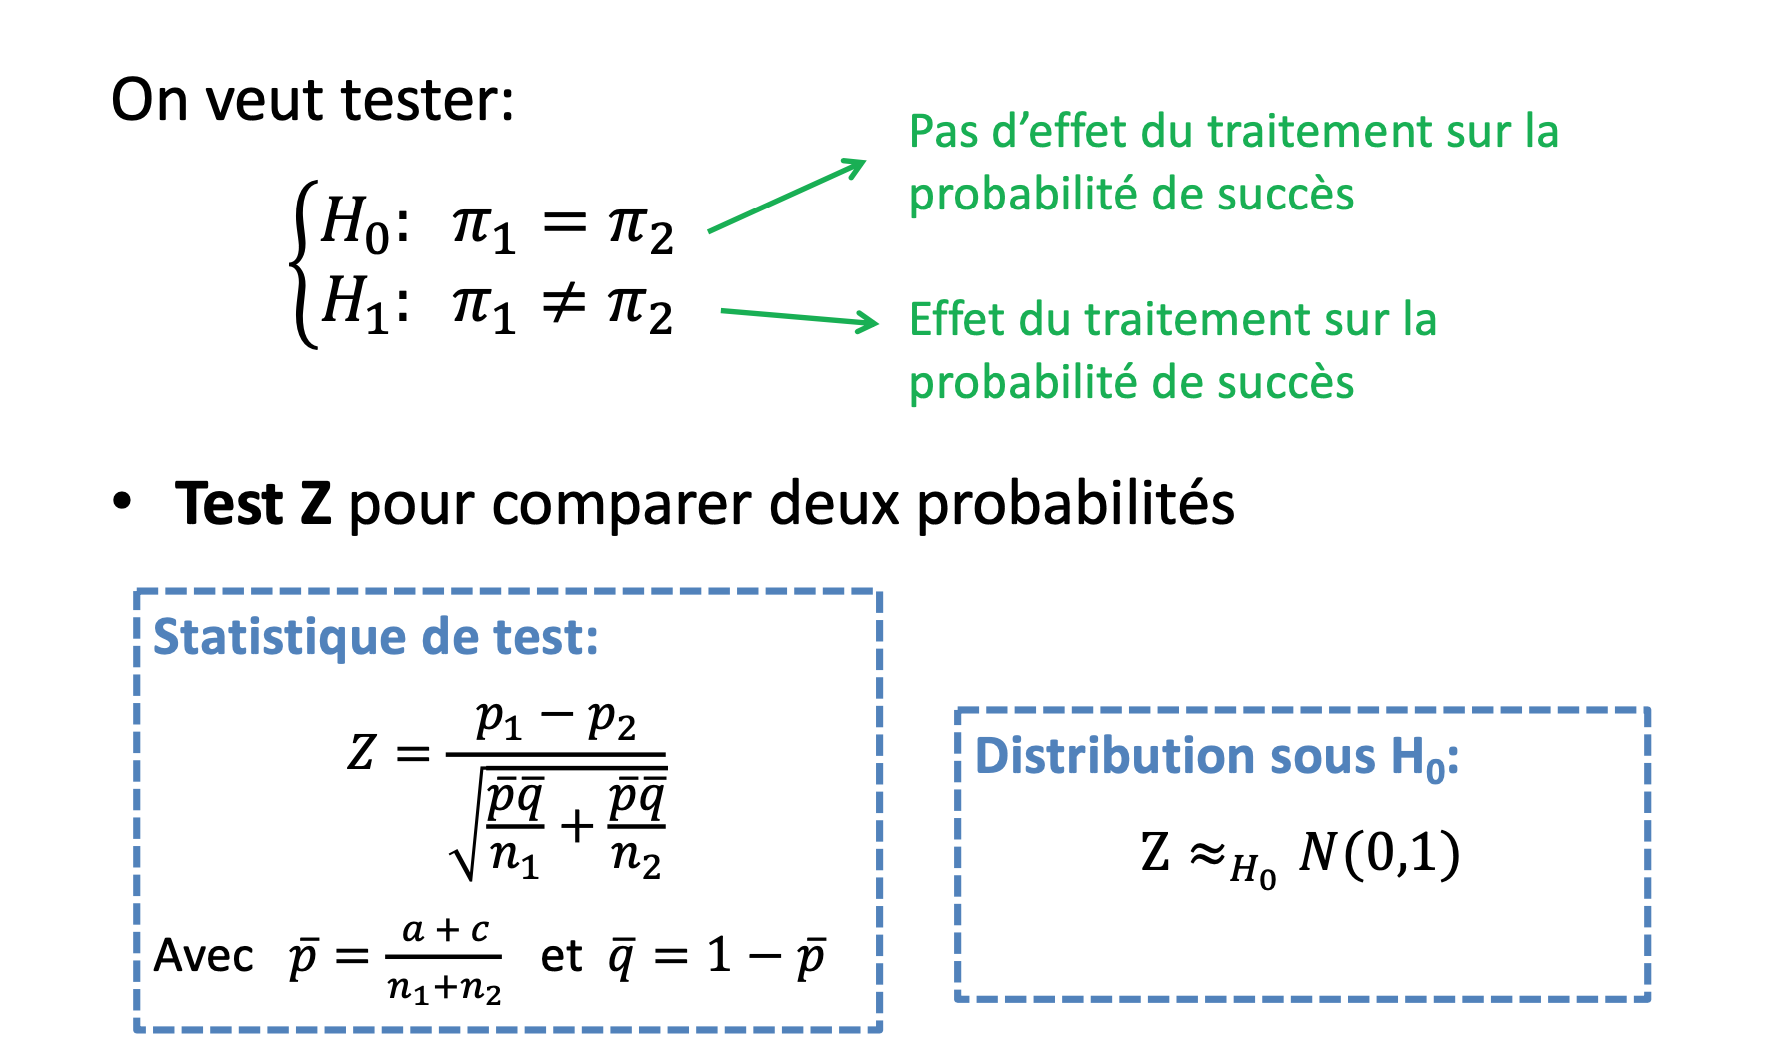
\includegraphics[scale=0.5]{images/testZ.png}
    \caption{Test Z pour comparer deux probabilités}
    \label{fig:my_label}
\end{figure}


\subsubsection{Test Chi-carré d’indépendance} 
\begin{figure}[H]
    \centering
    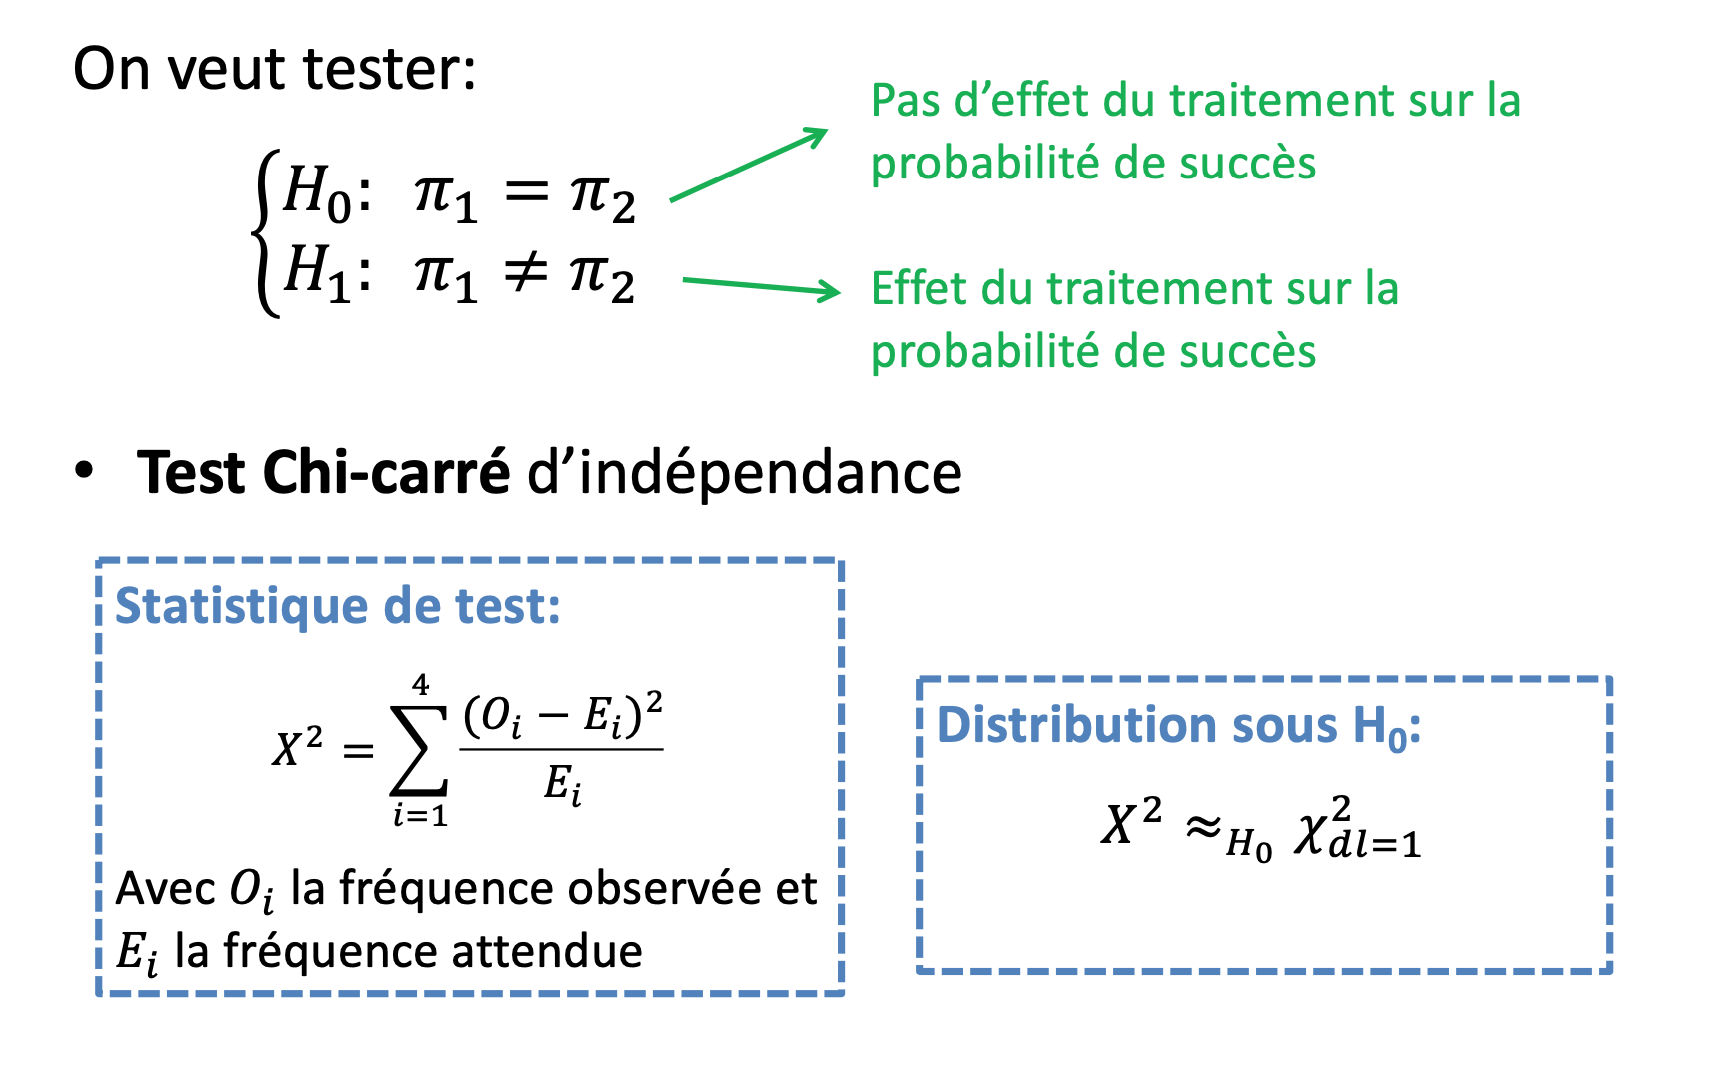
\includegraphics[scale =0.5]{images/testchisquare.png}
    \caption{Test Chi carré d'indépendance}
    \label{fig:my_label}
\end{figure}

\subsubsection{Remarques}
\begin{enumerate}
    \item Le test chi-carré est en fait équivalent au test Z, basé sur l’approximation normale de la distribution binomiale.
    $$X^{2} = (Z)^{2}$$
    \item Il existe aussi un test chi-carré avec une correction de continuité
    \begin{itemize}
        \item La statistique de test classique ne peut en réalité prendre qu’un nombre discret de valeurs alors que la distribution théorique (chi-carré) est une distribution continue.
        \item Le calcul de la P-valeur est approximatif, et on ne peut donc ne pas exactement contrôler $\alpha$ (surtout lorsque dl=1).
        \item Il est alors recommandé d’utiliser la correction de continuité de Yates (Yates,1934) Figure \ref{fig:Yates}.
    \end{itemize}
    \item Ces résultats reposent sur le TCL et sont asymptotiques.
    \begin{itemize}
        \item Si taille d’échantillon petite, mais toutes les fréquences attendues >5 : test chi-carré OK avec correction de continuité de Yates
        \item Si au moins une fréquence attendue $\leqslant 5$, alors le test chi-carré et le test Z ne peuvent pas être utilisé. On peut alors réaliser un test exact de Fischer
    \end{itemize}
\end{enumerate}

\begin{figure}[H]
    \centering
    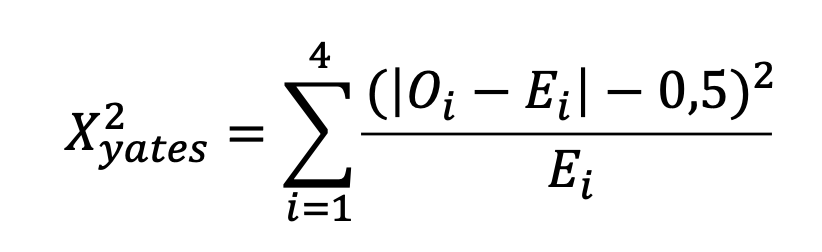
\includegraphics[scale = 0.5]{images/Yates.png}
    \caption{Correction de continuité de Yates}
    \label{fig:Yates}
\end{figure}

\subsubsection{Cas des données pairées}

\begin{figure}[H]
    \centering
    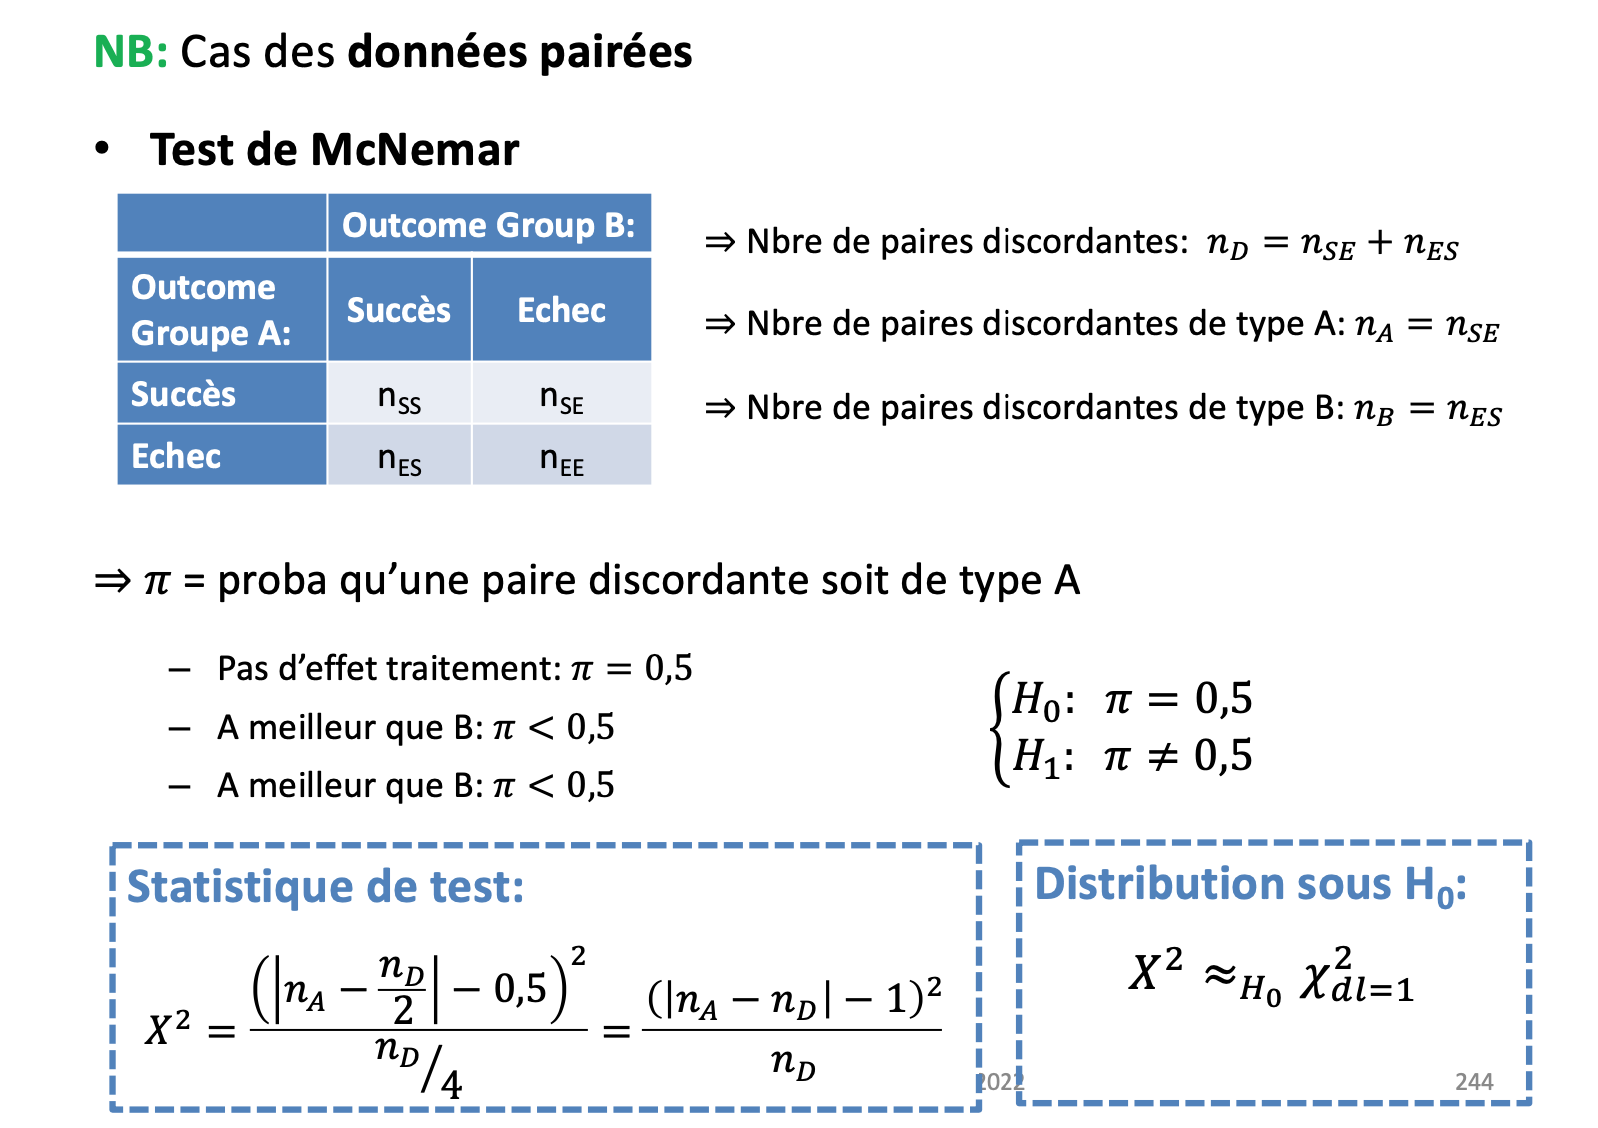
\includegraphics[scale = 0.5]{images/donnespaires.png}
    \caption{Test statistique dans le cas de données pairées}
    \label{fig:paires}
\end{figure}

\subsection{Estimation effet traitement}

Différentes possibilités :
\begin{itemize}
    \item Différence des proportions estimées
    \item Rapport de risques (Risks ratio, RR) estimé
    \item Rapport de cotes (Odds ratio, OR) estimé
\end{itemize}

\subsubsection{Différence des proportions estimées}
Cette technique consiste à faire la différence entre les deux probabilités de succès. Mais c'est rarement utilisé !

\subsubsection{Rapport de risques (Risks ratio, RR) estimé}
Cette technique revient à faire le ratio des proportions estimées. Le RR peut se calculer dans les études prospectives (et donc dans les essais cliniques) mais pas dans les études rétrospectives de type cas-contrôle.
$$\hat{RR} = \frac{\hat{\pi_{1}}}{\hat{\pi_{2}}}=\frac{p_{1}}{p_{2}} $$
Pour l'interprétation :
\begin{figure}[H]
    \centering
    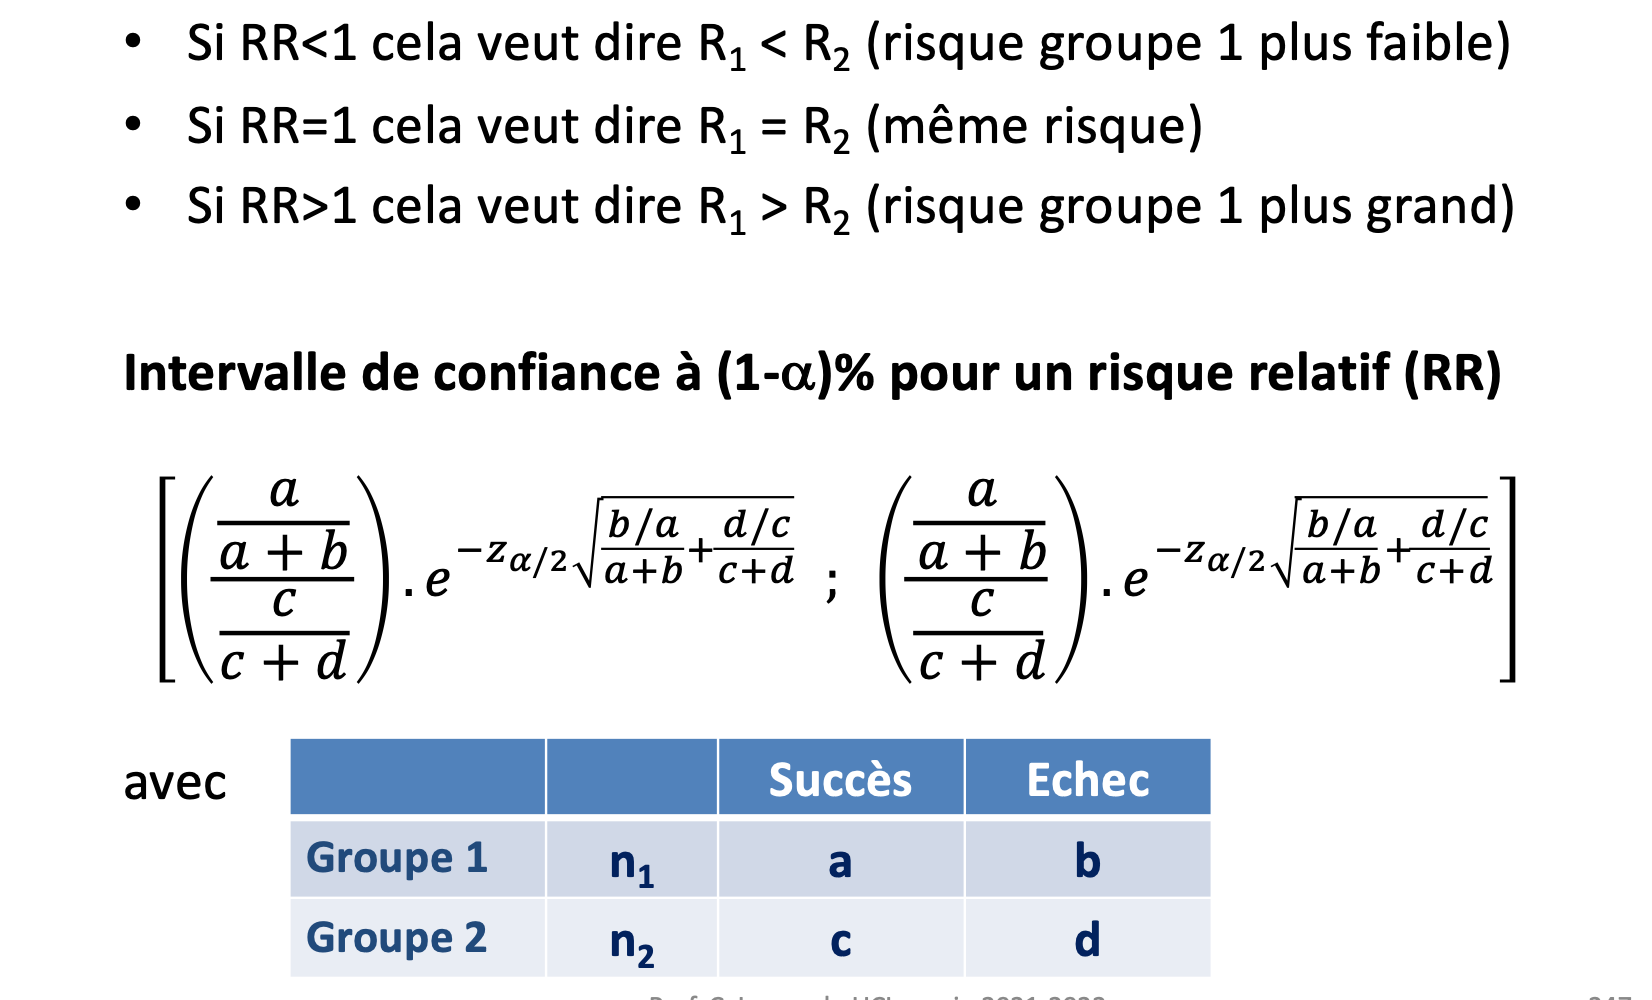
\includegraphics[scale = 0.5]{images/interpretationrisqueration.png}
    \caption{Interprétation du rapport de risque}
    \label{fig:my_label}
\end{figure}

\subsubsection{Rapport de cotes (Odds ratio, OR) estimé}

Cote = probabilité de succès sur probabilité d’échec.

\begin{figure}[H]
    \centering
    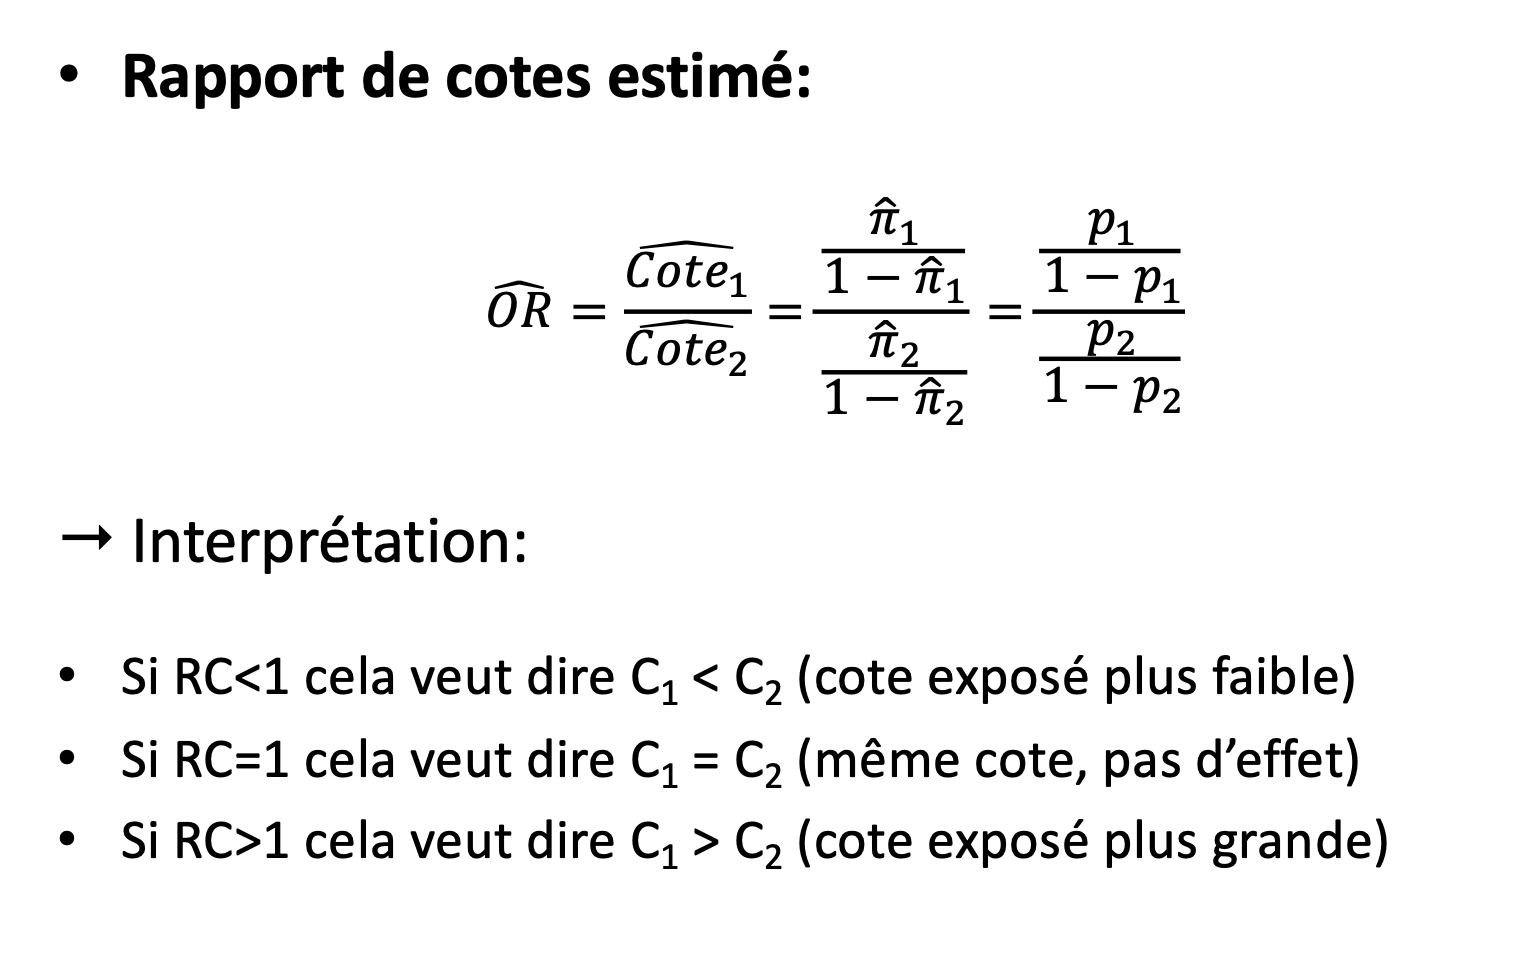
\includegraphics[scale=0.5]{images/rapportdescotes.png}
    \caption{Interprétation rapport des côtes}
    \label{fig:my_label}
\end{figure}


\begin{figure}[H]
    \centering
    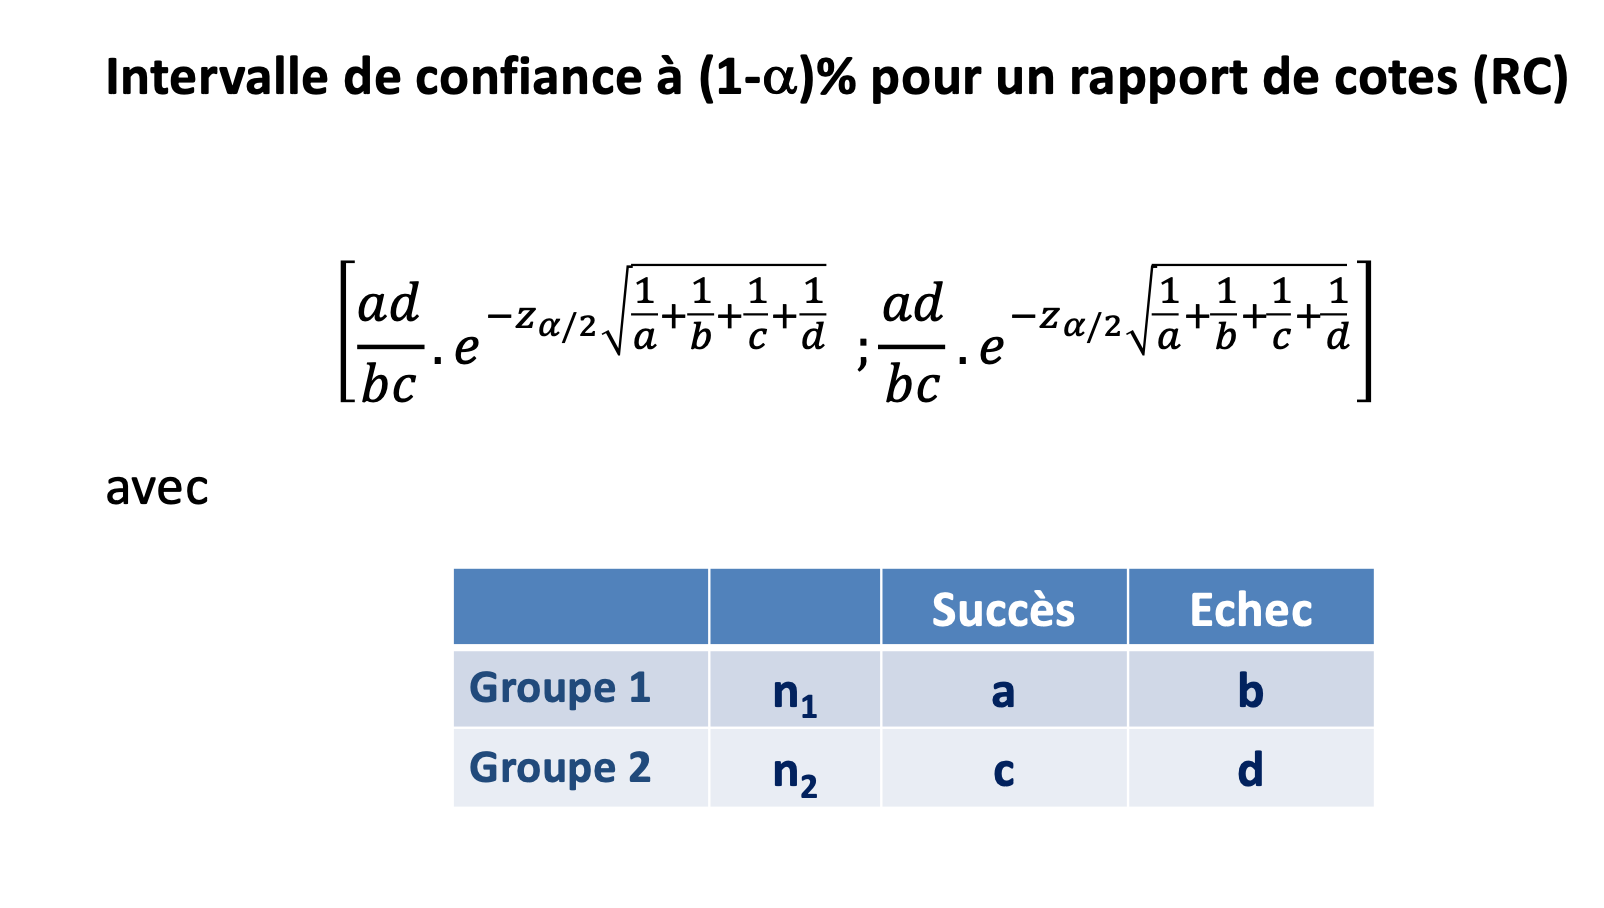
\includegraphics[scale=0.5]{images/intervaldeconfiance.png}
    \caption{Intervalle de confiance du rapport des côtes}
    \label{fig:my_label}
\end{figure}
Il faut attention à la manière d'interpréter le RR et OR. Ils ont la même interprétation qualitative, mais pas quantitative.
\begin{figure}[H]
    \centering
    
\includegraphics[scale =0.3]{images/RROR.png}
    \caption{Interprétation RR et OR}
    \label{fig:RROR}
\end{figure}
\subsection{Régression logistique}
On ne peut pas faire une régression linéaire, car nous avons une variable de réponse binaire Y (= 0 pour échec ou 1 pour succès) et un ou plusieurs facteurs : $X=(X_{1}, ..., X_{k})$\\

On voudrait modéliser le risque $\pi = P(Y=1|X)$. Mais En réalité, on va modéliser le logarithme de la cote, c.-à-d. le logit de $\pi$.

\begin{figure}[H]
    \centering
    
\includegraphics[scale = 0.3]{images/logit.png}
    \caption{Formule logit}
    \label{fig:my_label}
\end{figure}

$$ logit(\pi) = \beta_{0}+\beta_{1}X_{1}+...+\beta_{n}X_{n}$$

\begin{figure}[H]
    \centering
    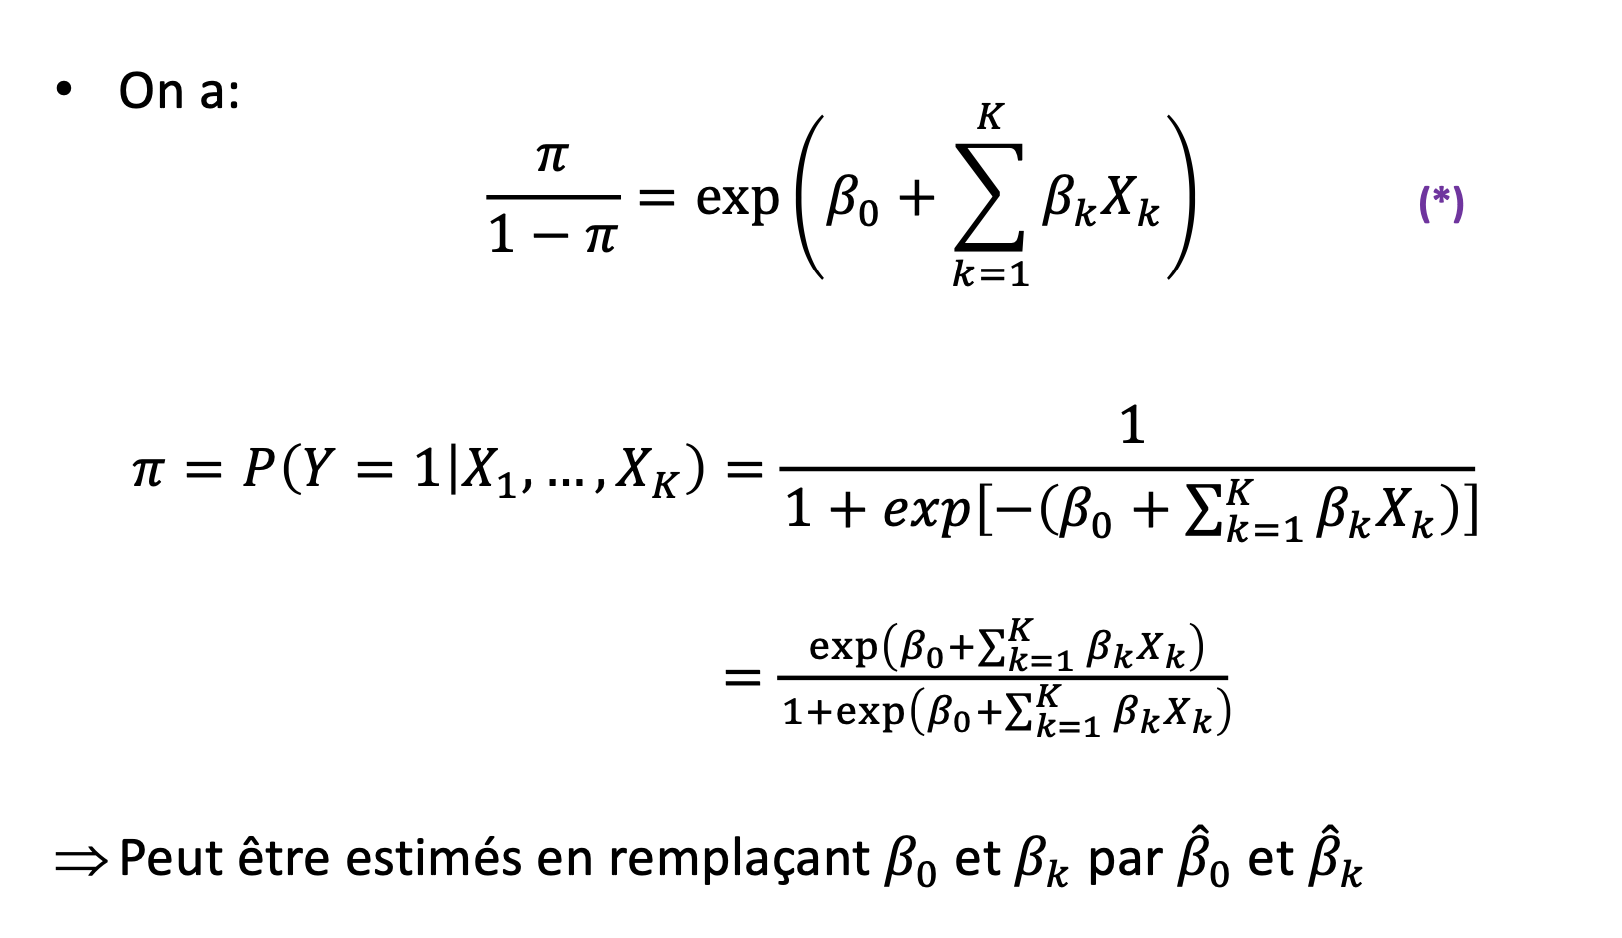
\includegraphics[scale=0.5]{images/pi_logit.png}
    \caption{Valeur de \pi pour logit régression}
    \label{fig:my_label}
\end{figure}

\begin{figure}[H]
    \centering
    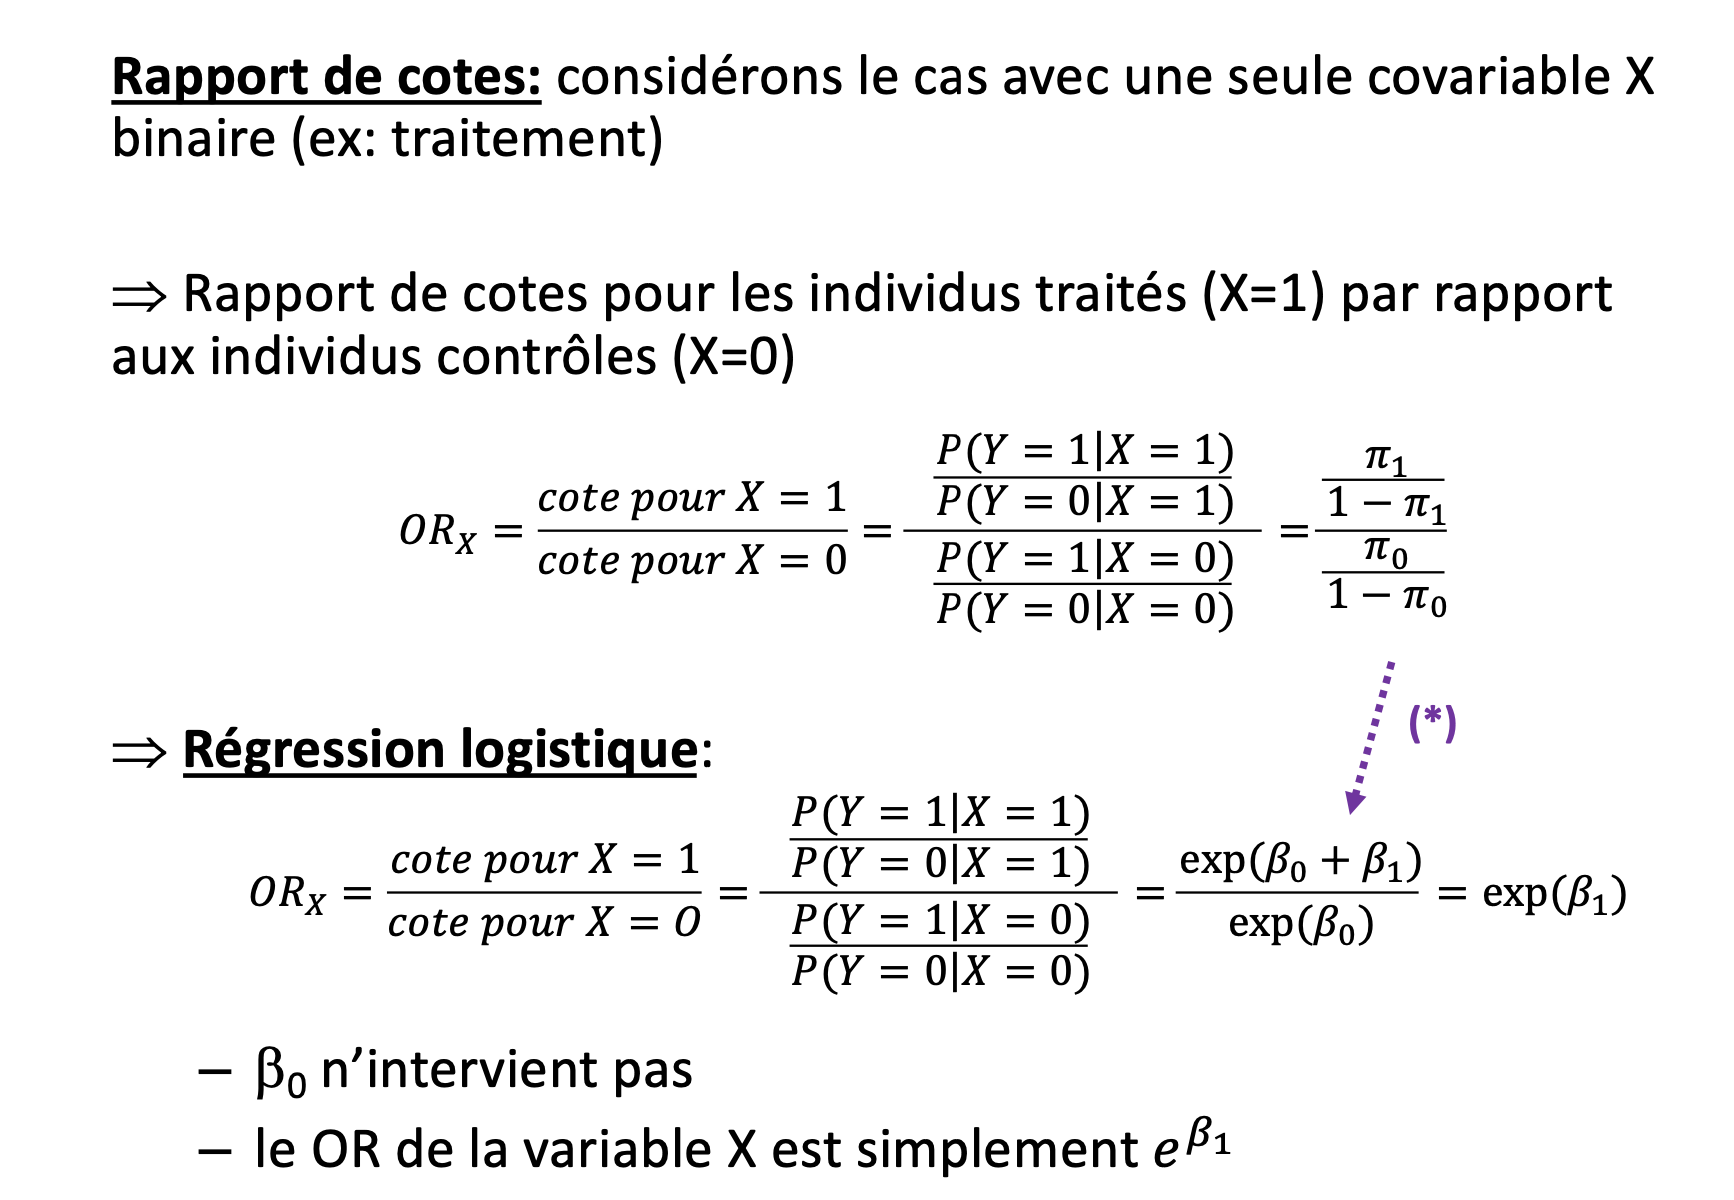
\includegraphics[scale=0.5]{images/rapportcote_logit.png}
    \caption{rapport des cotes en logit régression}
    \label{fig:my_label}
\end{figure}

\subsubsection{Estimation des paramètres}
L’estimation des paramètres peut se faire en appliquant le principe du maximum de vraisemblance. 
\begin{figure}[H]
    \centering
    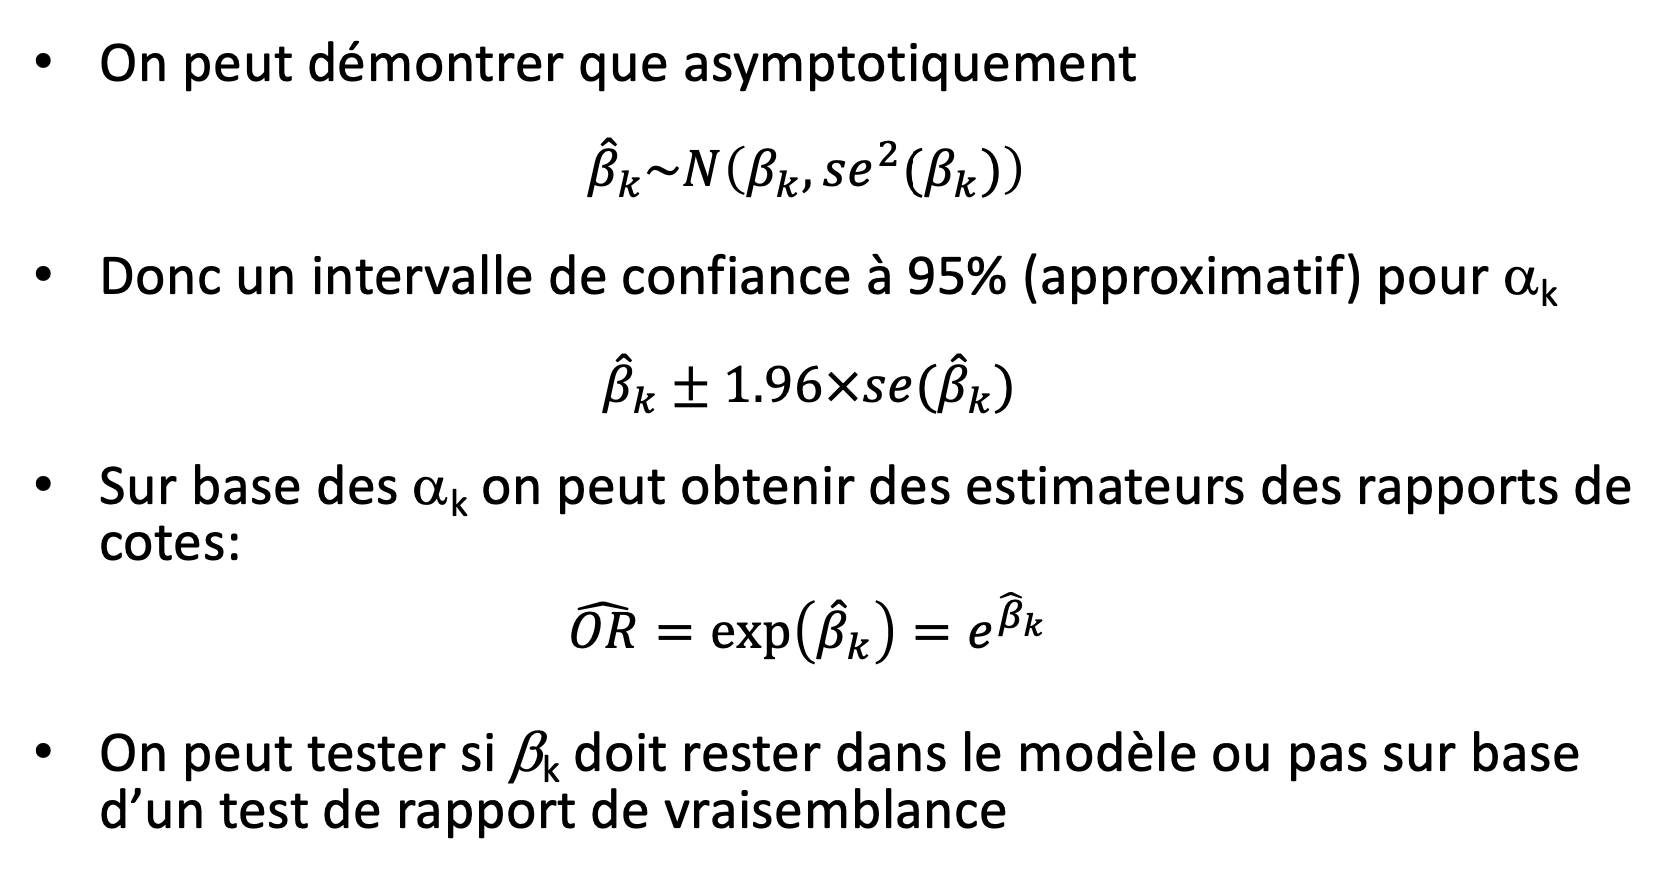
\includegraphics[scale =0.5]{images/estimation_logit.png}
    \caption{estimation des paramètres pour logit régression}
    \label{fig:my_label}
\end{figure}
\subsubsection{Test du maximum de vraisemblance}

\begin{figure}[H]
    \centering
    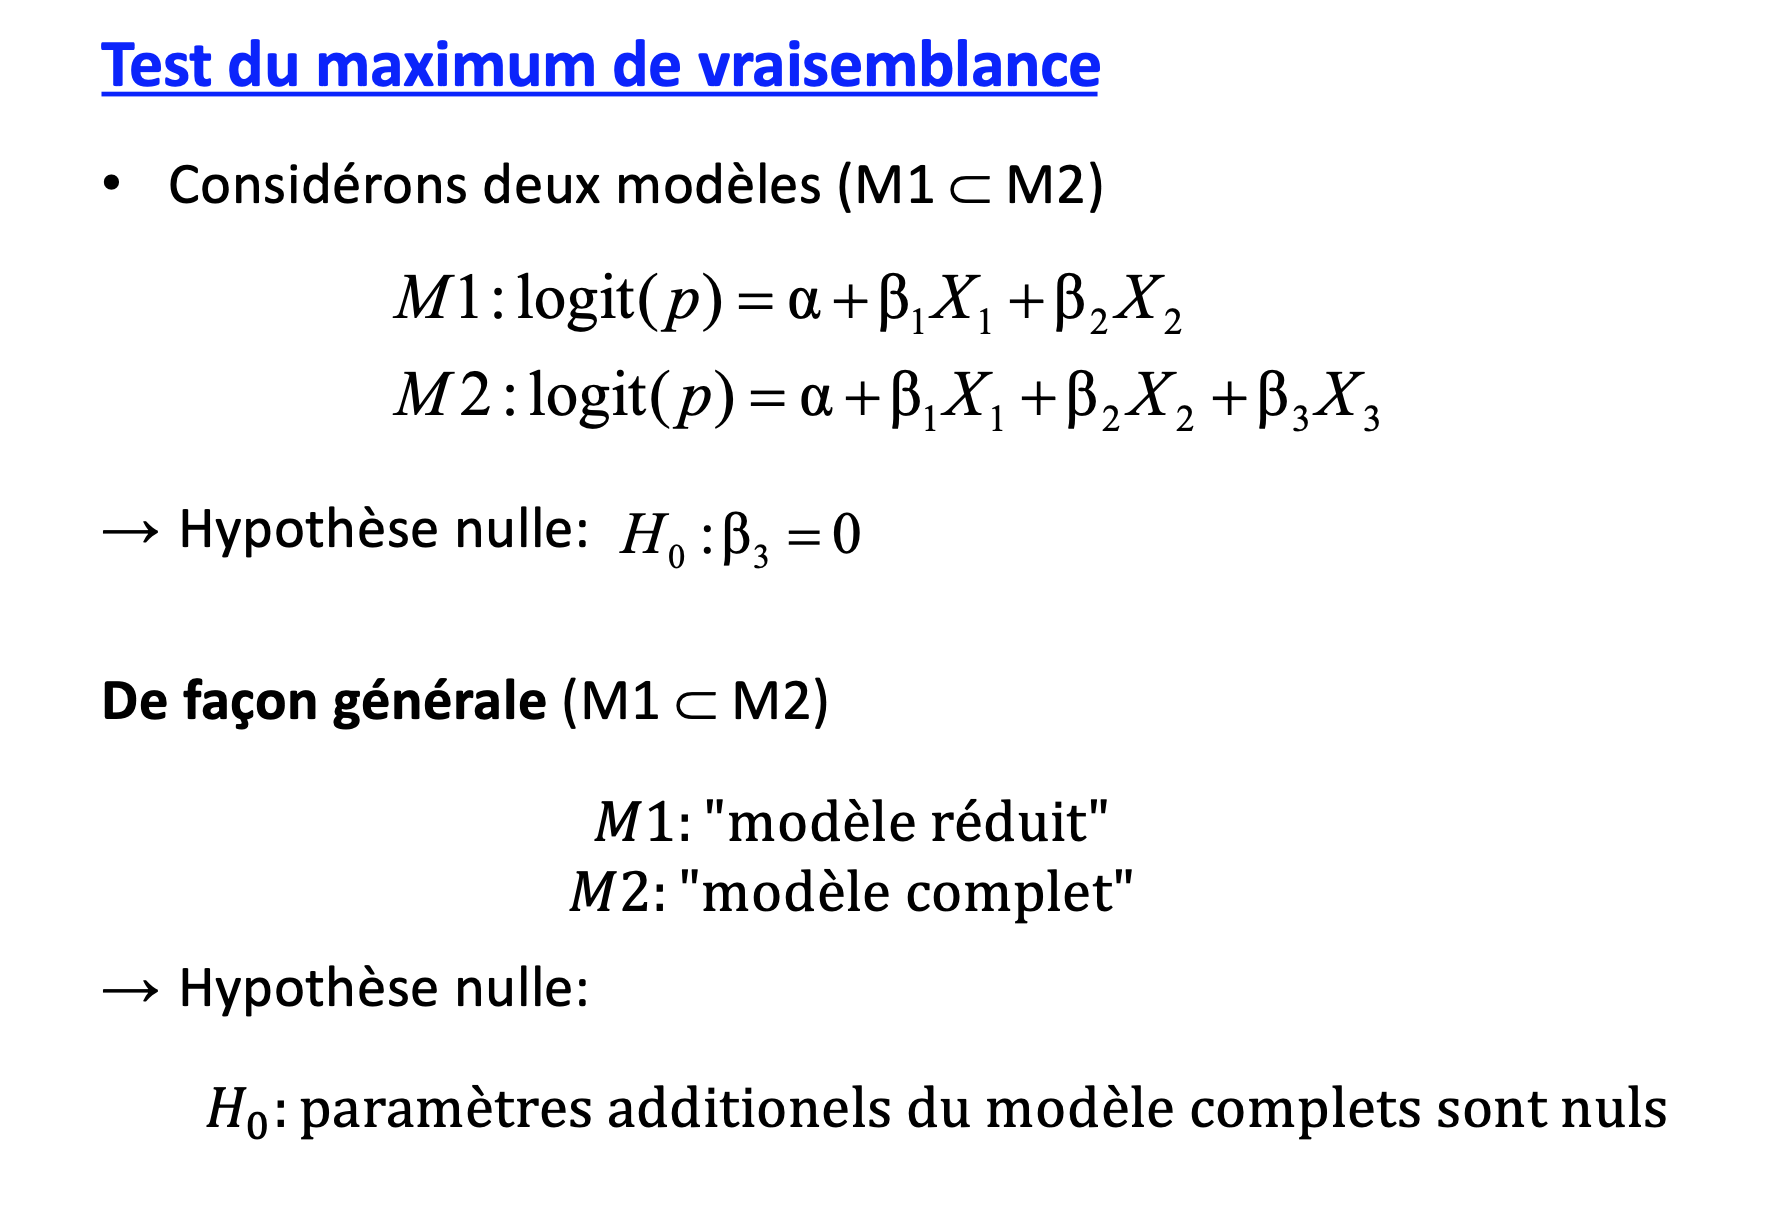
\includegraphics[scale = 0.5]{images/test_vraisemblance.png}
    \caption{Test du maximum de vraisemblance}
    \label{fig:my_label}
\end{figure}
\subsubsection{Test de Wald}
\begin{figure}[H]
    \centering
    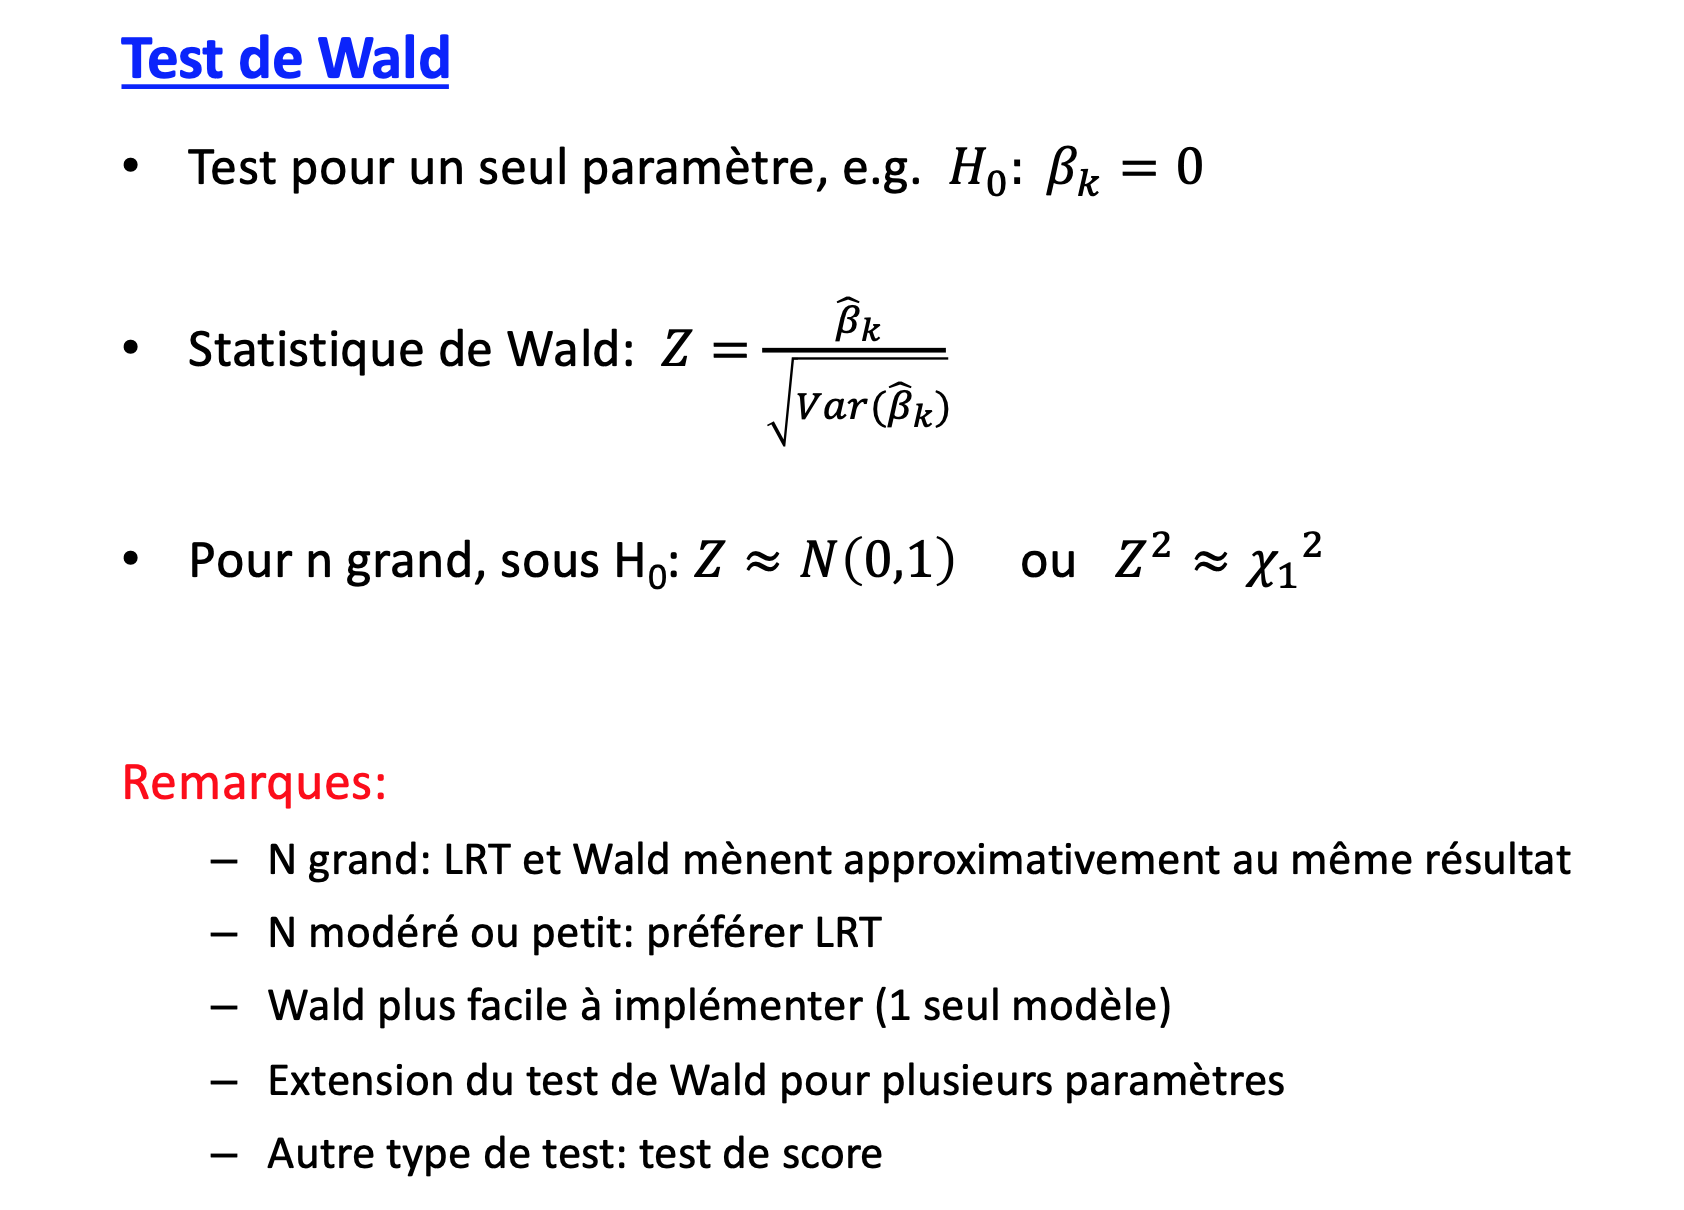
\includegraphics[scale = 0.5]{images/test_wald.png}
    \caption{Test de Wald}
    \label{fig:my_label}
\end{figure}
\subsection{Cas de plus de 2 groupes de traitement}
Soit, on peut faire une Comparaison globale et cela revient à une généralisation directe du test chi-carré pour une table de contingence $r×c$. Soit, on fait des comparaisons deux à deux mais cela implique un problème de multiplicité de test. Le même type de solutions que précédemment peut être utilisé. 

\section{Endpoint de survie}
Pour chaque patient : temps entre une origine et un événement prédéfini (exemple survie). On a une variable continue positive. Mais Au moment de la fin de l'étude, l'événement d'intérêt n'est généralement pas observé pour tous les patients. On parle dans ce cas-là de \textbf{données censurées (à droite)}. Il faut faire attention que ce processus de censure doit être indépendant de l'apparition des événements analysés (donc une censure administrative, c'est ok).


\subsection{Résumer des données de survie}
Méthodes "classiques" (moyenne, histogrammes, …) ne
fonctionnent pas (à cause de la censure !)\\
On peut utiliser une fonction de survie : 
$$S(t) = P(T>t)$$
$S(t)$ représente pour chaque instant t la probabilité que le temps jusqu'à l'événement soit le plus grand que cet instant. On va utiliser une représentation graphique de l'estimateur de la fonction de survie= \textbf{Estimateur de Kaplan-Meier} qui se calcule de la manière suivante :
$$\widehat{S}(t) = \prod_{j=0}^t (1-\frac{O_{j}}{n_{j}})$$
Un exemple est donné dans les slides.

\subsection{Effet traitement}
Pour mesurer l'effet d'un traitement, on va utiliser les éléments suivants.
\subsubsection{Test du Logrank}
On va comparer les courbes de survie pour 2 groupes.
On définit :
\begin{itemize}
    \item Groupe 1 = groupe expérimental $S_{exp}(t)$
    \item Groupe 2 = groupe standard $S_{std}(t)$
\end{itemize}
On va avoir comme test d'hypothèse :
\begin{figure}[H]
    \centering
    
\includegraphics[scale = 0.5]{images/logrank.png}
    \caption{test d'hypothèse pour un test du Longrank}
    \label{fig:my_label}
\end{figure}

\subsection{Hazards ratio (HR)}
Cela permet d'estimer le rapport de risques d'événement entre deux groupes. 
\begin{figure}[H]
    \centering
    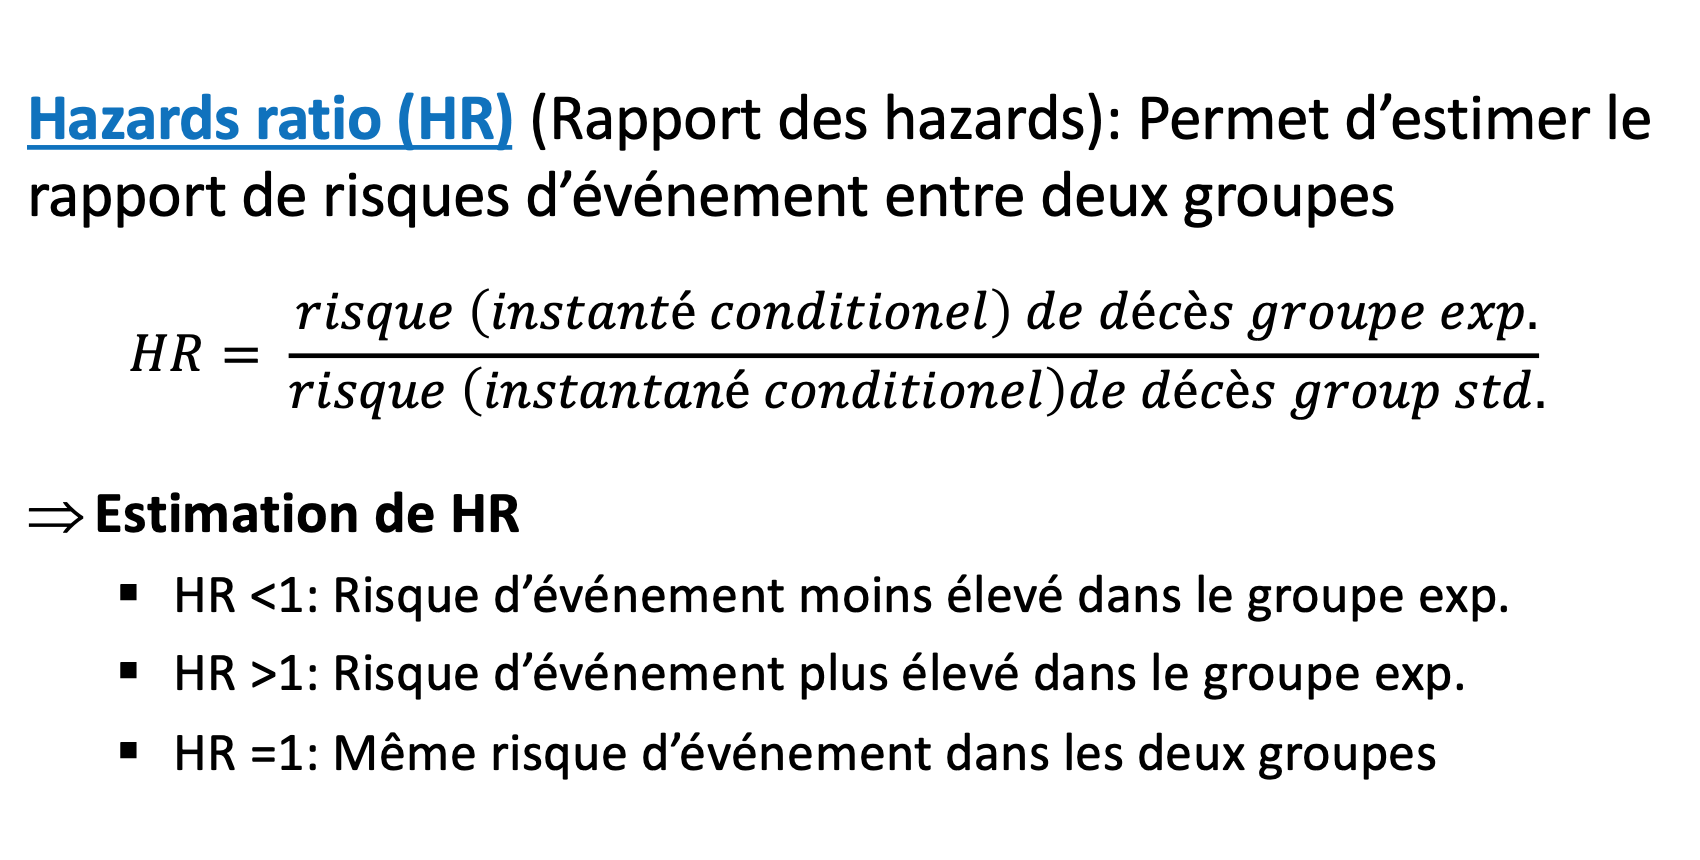
\includegraphics[scale=0.5]{images/hazardratio.png}
    \caption{Hazard ratio (HR)}
    \label{fig:my_label}
\end{figure}

\subsection{Modélisation des données de survie}
Il existe plusieurs modèles de régression s’appliquant aux données de survie, le plus connu est le modèle de Cox (modèle de hazards proportionnels).

\subsection{Modèle de Cox}
Modèle semi-paramétrique, car on a un terme qui dépend que du temps et l'autre des paramètres.
\begin{figure}[H]
    \centering
    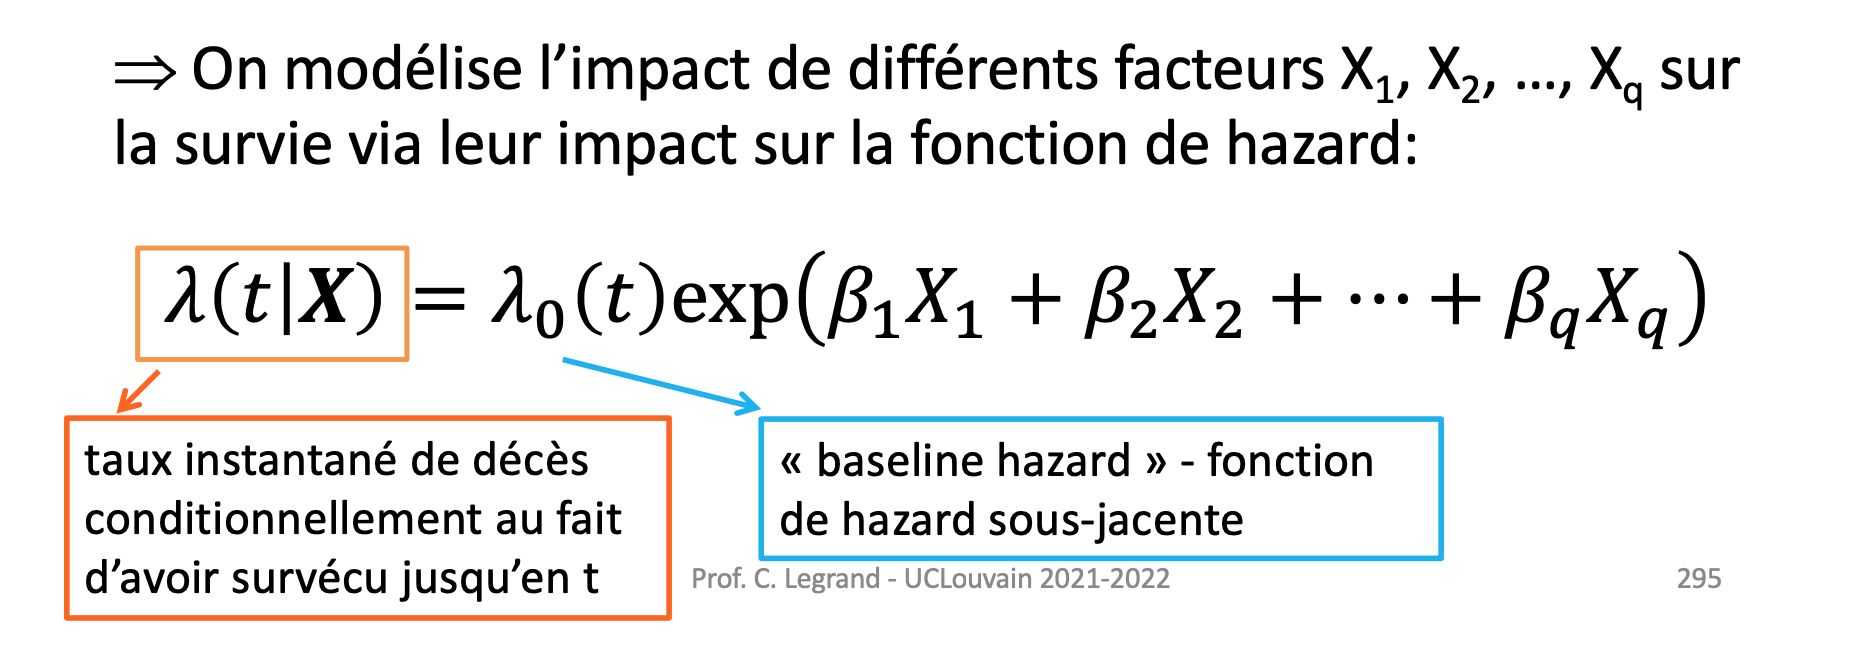
\includegraphics[scale=0.5]{images/modelecox.png}
    \caption{modèle de Cox}
    \label{fig:my_label}
\end{figure}

Quelques résultats importants :

\begin{figure}[H]
    \centering
    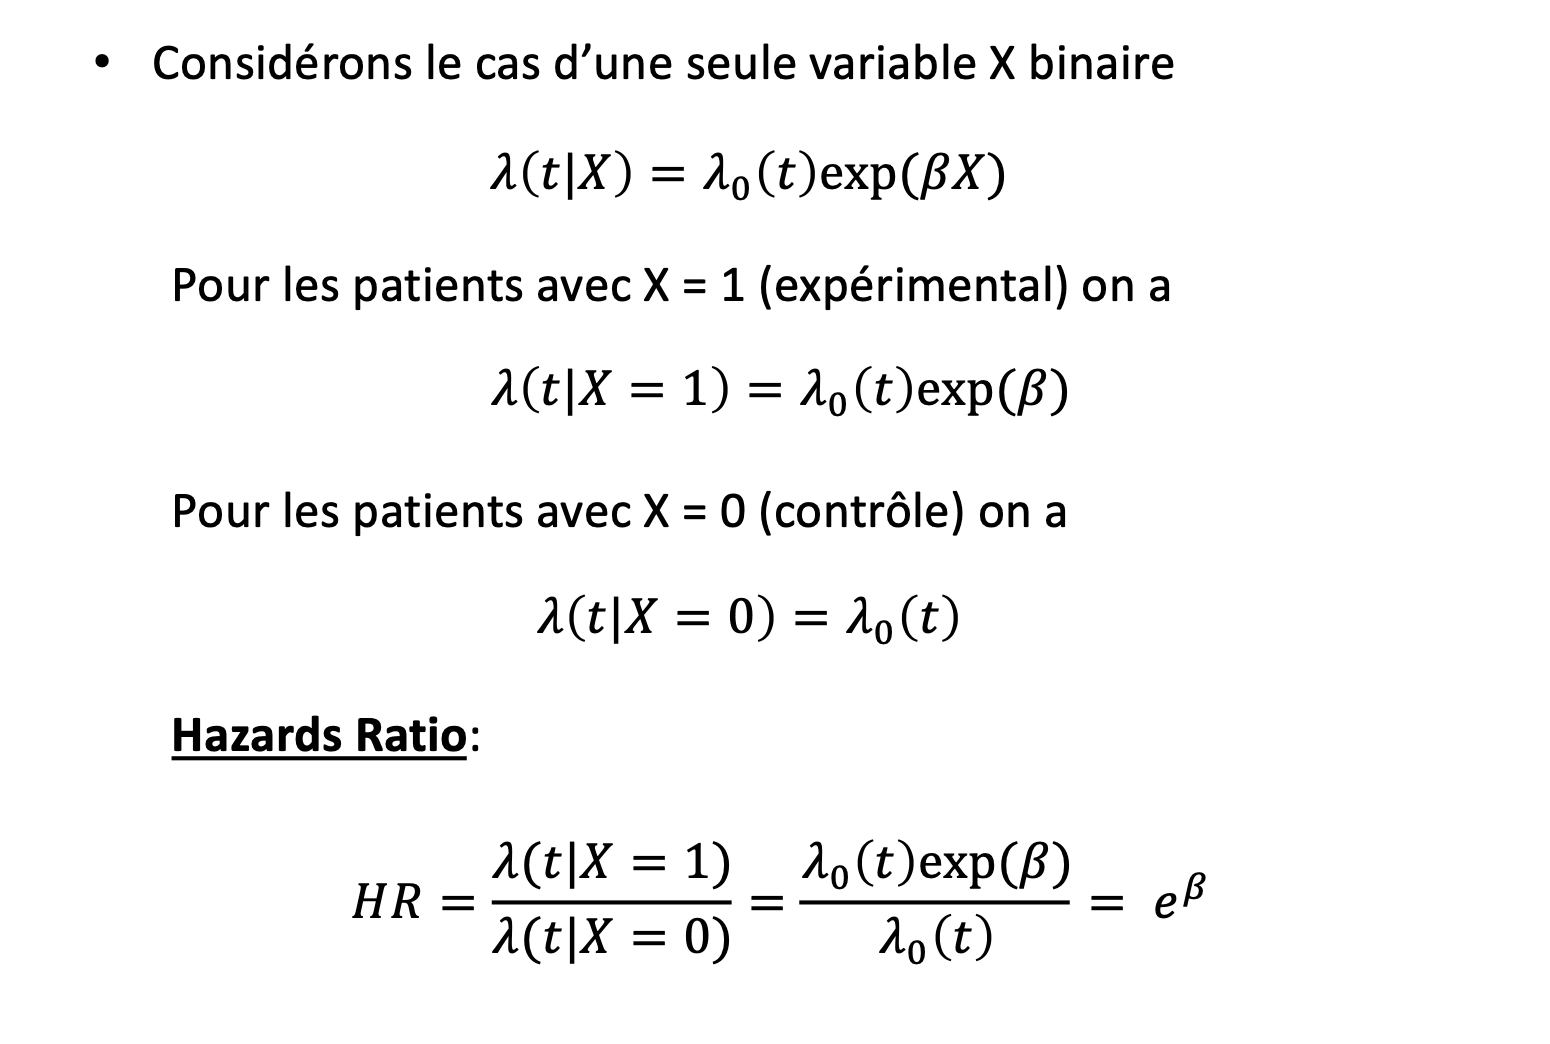
\includegraphics[scale=0.5]{images/cox_1.png}
    \caption{Résultat avec modèle de Cox}
    \label{fig:my_label}
\end{figure}

\begin{figure}[H]
    \centering
    \includegraphics[scale=0.5]{images/cox_2.png}
    \caption{Résultat avec modèle de Cox}
    \label{fig:my_label}
\end{figure}

\begin{figure}[H]
    \centering
    \includegraphics[scale=0.5]{images/cox_3.png}
    \caption{Résultat avec modèle de Cox}
    \label{fig:my_label}
\end{figure}

\subsection{Code R}
voir slides



\chapter{Phase III - Calcul de taille d'échantillon}

\section{Est-ce important ?}
Dans cette section, on va discuter de l'importance de calculer la taille d'échantillon pour réaliser un essai clinique de phase III.
Un rappel assez bref : \\

\textbf{Phase III}: comparer 2 (ou >2) traitements dans un échantillon de pts\\

\textbf{But}: généraliser nos conclusions à la population

\subsection{Important d’un point de vue méthodologique}
\begin{itemize}
    \item En général, échantillon hétérogène de patients
    \item Une différence observée peut être dû à la chance uniquement
    \item On peut ne pas observer dans notre échantillon une différence existant réellement.
\end{itemize}

\vspace{0.18cm}

\textbf{Les traitements doivent être donnés à un échantillon de patients suffisamment grand pour être représentatif de la population, et de taille adéquate pour contrôler les risques d’erreur de type I et II.}

\subsection{Important pour une utilisation optimale des ressources}
\begin{itemize}
    \item Si trop peu de pts : perte de temps, d’argent et d’efforts, car il est peu probable qu’une telle étude mette au jour des améliorations cliniques
    \item Si trop de pts : gaspillage de temps, d’argent et d’efforts.
\end{itemize}

\subsection{Important d’un point de vue éthique}
\begin{itemize}
    \item Si trop peu de pts : perte de temps, d’argent et d’efforts, car il est peu probable qu’une telle étude mette au jour des améliorations cliniques
    \item Si trop de pts : gaspillage de temps, d’argent et d’efforts.
\end{itemize}

\section{De quoi dépend la taille d’échantillon ?}
\begin{itemize}
    \item Objectif et design de l’essai
    \item Type d’endpoint
    \item Contrôle du risque d’erreur de type I et II (puissance) 
    \item Taille de l’effet traitement que l’on veut mettre en évidence
\end{itemize}

\vspace{0.15cm}

 La taille d’échantillon est déterminée pour obtenir une grande puissance pour détecter un effet du traitement de taille donnée avec un faible risque d’erreur de type I.
 
\subsection{En pratique}
On va se fixer un risque d’erreur de type II ($\beta$), ou de façon équivalente une puissance ($1 − \beta$) pour une alternative prédéfinie et on calcule la taille d’échantillon nécessaire n pour contrôler ce risque à cette valeur.\\

\textbf{Attention aux éléments suivants :}
\begin{itemize}
    \item Si en réalité l’effet du traitement dans la population est plus petit ($< \delta$) alors la puissance sera plus faible que prévu
    \item Si en réalité l’effet du traitement dans la population est plus grand ($> \delta $) alors la puissance sera plus grande que prévu
    \item Avec une taille d’échantillon suffisamment grande même une très petite différence peut être significative
\end{itemize}

\vspace{0.15cm}

\begin{center}
    \textbf{Statistiquement significatif ≠ Cliniquement significatif}
\end{center}

\subsection{Taille de l’effet traitement}
\textbf{Effet traitement cliniquement significatif : }Pour convaincre la communauté médicale de changer leur pratique, il faut démontrer non pas une amélioration, mais bien une amélioration clinique valant la peine de changer la façon de traiter les patients.\\
\textbf{Effet traitement plausible : }L’effet traitement que l’on cherche à mettre en évidence doit être plausible et réaliste.\\

\subsection{Erreur de type I et II}


\section{Comparaison de deux proportions}
\begin{figure}[H]
    \centering
    \includegraphics[scale=0.5]{images/comparasion2proportions.png}
    \caption{Comparaison de deux proportions}
    \label{fig:comp2propor}
\end{figure}
La fonction en R : \textbf{power.prop.test}

\section{Comparaison de deux moyennes}
\begin{figure}[H]
    \centering
    \includegraphics[scale =0.5]{images/comparaison2moyennes.png}
    \caption{Comparaison de deux moyennes}
    \label{fig:comp2moyennes}
\end{figure}
\section{Comparaison de deux courbes de survie}
\begin{figure}[H]
    \centering
    \includegraphics[scale=0.5]{images/comparasion2courbes.png}
    \caption{Comparaison de deux courbes de survies}
    \label{fig:survie}
\end{figure}

\textbf{Dans le cas des données de survie, la puissance n’est pas déterminée par le nombre de patients, mais bien par le nombre d’événements!}
\section{Remarques générales}
Quelques remarques : 
\begin{itemize}
    \item Plusieurs logiciels disponibles:
    \begin{itemize}
        \item Packages/fonctions R, macro/procédure SAS
        \item Packages spécifiques (EAST, Nquery, ...)
    \end{itemize}
\item Parfois plusieurs formules disponibles (solutions approximatives), dans certains cas plus compliqués il n’existe pas de formules ($\Rightarrow simulations$)
 \item Situations plus compliquées si analyses intérimaires (Procédure séquentielle).
\end{itemize}



\chapter{PHASE III - IDMC et analyses intérimaires}

\section{Idée générale}
Un essai clinique de phase III dure souvent plusieurs années, on a donc la nécessité de s’assurer que « tout va bien » pendant l’essai.
\begin{figure}[H]
    \centering
    \includegraphics[scale = 0.4]{images/IDMC.png}
    \caption{IDMC: idée générale}
    \label{fig:IDMC}
\end{figure}
Sauf qu'inspecter(régulièrement) les données par groupe est problématique pour différentes raisons :
\begin{itemize}
    \item Problèmes avec l’aveugle
\item Risque de sur-interprétation des résultats et de démotivation
pour l’essai en cours
\item Risque de suspicion de fraude (si des actions sont/doivent être prises)
\item Problème de méthodologie statistique (tests multiples).
\end{itemize}

\vspace{0.5cm}

\begin{center}
    $\Rightarrow$ Independent Data Monitoring Committee (IDMC)
\end{center}
\section{IDMC}


\section{Analyses intérimaires}

\begin{itemize}
    \item Toute une série de points n’ont pas d’impact sur la méthodologie statistique de l’essai :
    \begin{itemize}
        \item Monitoring des données individuelles des patients
\item Monitoring du recrutement, des centres actifs, de la participation des
investigateurs, etc
\item Monitoring des aspects logistique (approvisionnement en médicaments, encodage des données, etc)
\item Monitoring global de la safety/toxicité des patients sans comparaison formelle par groupe
    \end{itemize}
\item Par contre, réaliser une comparaison formelle des bras de traitement requiert une méthodologie adaptée !
– Contrôle du risque d’erreur de type I
\end{itemize}
\subsection{Problème de multiplicité}
On sait que le risque global d’erreur de type I augmente (très rapidement) avec le nombre de comparaisons.

\subsection{Analyses intérimaires : Comment contrôler le risque d’erreur de type I global}

L'idée est de diviser le $\alpha$ sur les différents tests réalisés(et prendre en compte la corrélation entre les statistiques de tests successives).


\chapter{Phase I - design et analyse}

La phase I d'un essai clinique est une phase cruciale pour les différentes raisons:

\begin{itemize}
    \item Première phase du développement clinique d’un nouveau traitement
    \item Concerne principalement les traitements médicamenteux
    \item Première administration du traitement chez des êtres humains. Soit des participants sains volontaires, soit des participants en stade avancé.
\end{itemize}

\vspace{0.25cm}
On peut la définir comme ceci :
\begin{center}
    \textbf{Determination of the maximal dose of drug, either alone or as part of a combination, that will, when administered by a specific schedule and route, produce an acceptable toxity.}
\end{center}
\vspace{0.25cm}

On parle aussi à cette étape d'essais cliniques non contrôlés car :
\begin{itemize}
    \item Pas de comparaison directe avec un autre traitement
     \item Pas de randomisation
      \item Tous les participants reçoivent le traitement étudié
\end{itemize}


\section{Objectifs}
Identifier la dose à étudier dans les phases suivantes du développement du traitement. Cela revient à identifier la plus forte dose produisant un taux acceptable de toxicité. On définit la \textbf{Dose maximum tolérée Maximum Tolerated Dose (MTD)} qui est la dose la plus élevée qui selon un design prédéfini est associée avec un taux "acceptable" de toxicité.\\

Le « taux acceptable de toxicité » dépend de la maladie traitée. En effet, pour des traitements en phase terminale, on accepte plus que pour des vaccins ou des traitements généraux.\\

On se base sur le paradigme "Dose-Intensité" :
Au plus la dose est élevée, au plus actif sera le traitement, mais également au plus toxique sera le traitement.\\

\begin{figure}[H]
    \centering
    \includegraphics[scale=0.3]{images/paradignmedoseintensite.png}
    \caption{Paradigme "Dose-Intensité"}
    \label{fig:dose_intensite}
\end{figure}

La \textbf{Dose Limiting Toxicity [DLT]} est une occurrence d’une toxicité inacceptable
\begin{enumerate}
    \item  Pas de définition universelle – dépend de la pathologie considérée
    \item Doit être défini clairement dans le protocole. 
    \item Souvent définie en termes de CTCAE like in the Figure \ref{CTCAE}
\end{enumerate}

\begin{figure}[H]
    \centering
    \includegraphics[scale =0.5]{images/CTCAE.png}
    \caption{CTCAE}
    \label{fig:CTCAE}
\end{figure}

\textbf{Dose maximum tolérée Maximum Tolerated Dose (MTD)} est la dose à laquelle la probabilité d’observer une DLT atteint un seuil donné.\\

La MTD est en général définie comme la proportion de cas de DLT :
$$Pr(DLT|MTD)=q_{0}$$

$q_{0}$ est généralement compris entre 0.1 et 0.4.\\

La MTD identifiée est ensuite utilisée comme dose de référence dans la suite du développement clinique (phase II).\\


\section{Contraintes}

\subsection{Contraintes pratiques}
seul un petit nombre de doses peuvent être observés par sujet. Cela a pour but d'éviter l'effet cumulatif des doses attribuées à un même patient, une longue période de « wash-out » étant en général pratiquement impossible.\\
Donc en général, une seule dose est testée sur chaque sujet.

\subsection{Contraintes éthiques}

On ne veut/peux pas exposer des patients à des doses associées à un niveau trop élevé de toxicité. On veut aussi éviter d'exposer des patients à des doses trop basses pour être efficaces. 

\section{Design}

\begin{figure}[H]
    \centering
    \includegraphics[scale=0.3]{images/designphase1.png}
    \caption{Différents designs en phase 1}
    \label{fig:designphase1}
\end{figure}

\subsection{Design classique 3+3}

\begin{figure}[H]
    \centering
    \includegraphics[scale=0.3]{images/3et31.png}
    \caption{Design 3+3}
    \label{fig:Design3et31}
\end{figure}

\begin{figure}[H]
    \centering
    \includegraphics[scale=0.3]{images/3et32.png}
    \caption{Design 3+3}
    \label{fig:Design3et32}
\end{figure}

\begin{figure}[H]
    \centering
    \includegraphics[scale=0.3]{images/3et33.png}
    \caption{Design 3+3}
    \label{fig:Design3et33}
\end{figure}
\subsubsection{Dose initiale $a_{1}$}
En général 1/10 de la $LD_{10}$(dose létale dans 10\% des souris traitées) pour la souris ajustée pour le poids. Pour les doses suivantes, on utilise des séquences mathématiques (Fibonacci, etc). 
\subsubsection{Inconvénients}
Cette méthode a des mauvaises propriétés statistiques.
\begin{figure}[H]
    \centering
    \includegraphics[scale=0.3]{}
    \caption{Statistique de 3+3}
    \label{fig:stat3+3}
\end{figure}
D'un point de vue statistique et éthique, on a une mauvaise utilisation de l’info. Seulement d'un point de vue éthique, cette méthode est très conservative et en pratique, c'est peu flexible.


\subsection{Continual Reassessment Method (CRM)}
Les objectifs de cette méthode sont de minimiser le nombre de pts traités à une dose trop faible ; de minimiser le nombre de pts traités à une dose trop haute ; de minimiser le nombre de pts total.

\subsubsection{Principes}
\begin{figure}[H]
    \centering
    \includegraphics[scale=0.3]{images/CRM.png}
    \caption{CRM principe}
    \label{fig:CRMprincipe}
\end{figure}

\begin{figure}[H]
    \centering
    \includegraphics[scale=0.3]{images/CRMdose.png}
    \caption{Choix de la douse}
    \label{fig:CRMdose}
\end{figure}

\subsubsection{Choix de la courbe dose-toxicité}
Il existe différentes fonctions continues monotones : exponentielle, logistique, probit, ...\\
En général, on prend des fonctions à 1 ou 2 paramètres, car on a peu de données (la courbe autorisée à se modifier seulement sous un seul aspect (en général la pente)). 


\section{Remarques}

\begin{itemize}
    \item On n’est pas concerné par une estimation précise de toute la courbe de dose-toxicité, mais uniquement par son adéquation à proximité de la MTD
    \item Il a été démontré que la technique CRM est robuste pour la détermination de la MTD, même sous un choix de courbe de dose- toxicité modérément incorrecte.
\end{itemize}
\chapter{Phase II - Design et analyse}


\section{Avant les phases II}

Avant les phases II, on a la phase I, les études PK/PD (pharmacokinetic / pharmacodynamic) et les  études précliniques.

\begin{itemize}
    \item Phase I
    \begin{itemize}
    \item MTD : Maximum Tolerated Dose : dose maximum pouvant
être administrée au patient
    \item Première idée du profil de toxicité.
\end{itemize}
\item études PK/PD (pharmacokinetic / pharmacodynamic)
\begin{itemize}
    \item Information sur l’absorption et l’élimination du traitement
     \item Permet de déterminer la dose et le schedule
d’administration pour maintenir la concentration du
traitement dans le sang, le plasma, …
\end{itemize}
\item études précliniques.
\end{itemize}



\section{Objectifs}

L'objectif de cette phase de l'essai clinique est d'évaluer l’activité thérapeutique du traitement sous une dose et un schédule déterminé et de compléter l’information disponible sur le profil de toxicité du traitement considéré. On veut savoir si l’activité du traitement est suffisant pour continuer le développement /l’investigation de ce traitement.

\section{Définition}

La définition la plus simple pour ce la phase II est 
\begin{center}
    \textbf{« It is to some extent easier to define phase II as the studies which are carried out following phase I assessment of a new agent but before large-scale assessment as part of a randomized phase III trial.}
\end{center}

Il y aussi différentes définitions/classifications ont été proposées:
\begin{itemize}
    \item Early Phase II versus Late Phase II
    \item Phase IIA versus Phase IIb
    \item Single agent Phase II versus Combined modality treatment Phase II
     \item Early Phase II versus Feasibility Phase II

\end{itemize}

\section{Analyse}

En général, on fait test d’hypothèse sur un « taux de réponse » par rapport à une norme considérée comme acceptable/inacceptable.\\
La taille d’échantillon est calculée sur base de deux taux de réponse :
\begin{itemize}
    \item P0 : le taux de succès en dessous duquel le traitement sera déclaré
inactif,
    \item P1 : le taux de succès au-dessus duquel le traitement sera déclaré
actif.
\end{itemize}

\section{Différents designs}

Il existe toute une série de designs et plusieurs améliorations/modifications ont été proposés dans la littérature.

Les plus courants sont : 
\begin{itemize}
    \item Gehan’s two stage design (1961)
    \item Fleming multiple-stage design (1982)
    \item Simon two-stage design (1989)
    \item Bryant and Day two-stage design (1995)
\end{itemize}

\subsection{Design de Gehan (1971)}
C'est un design en deux étapes et non randomisé. 

\subsubsection{étape 1}

Lors de l'étape 1, on a $n_{1}$ patients sont traités et on calcule $Y{1}$ = nombre de patients parmi les $n_{1}$ pour lesquels une activité thérapeutique du traitement a été observé (endpoint). 

On a ainsi la règle de décision :
\begin{itemize}
    \item Si Y1 = 0 on arrête l’étude et le développement clinique du traitement
    \item Si Y1 > 0 on continue l’étude
\end{itemize}
\begin{figure}[H]
    \centering
    \includegraphics[scale = 0.3]{images/gehan1.png}
    \caption{Gehan: étape 1}
    \label{fig:gehan1}
\end{figure}

\subsubsection{étape 2}
n2 patients sont traités de façon à obtenir une estimation de $\pi$
avec une erreur standard maximum donnée $\sigma_{M}$ (dans
l’échantillon global : $n = n_1 + n_2$)

\begin{figure}[H]
    \centering
    \includegraphics[scale = 0.3]{images/gehan2.png}
    \caption{Gehan: étape 2}
    \label{fig:gehan2}
\end{figure}

\subsection{Design de Fleming (1982)}
C'est une amélioration du design de Gehan. 

\subsection{Two-stage Simon design (1989)}
C'est un design en deux étapes. On considère que le traitement ne peut pas être accepté après la $1^{1}$ étape. 
\subsubsection{Étape 1}
on recrute n1 patients
\begin{itemize}
    \item Si r1 réponses ou moins : on arrête l’étude et on recommande de ne
pas poursuivre le développement
     \item Si plus de r1 réponses : on passe à l’étape 2 
\end{itemize}
\subsubsection{Étape 2}
on recrute n2 patients supplémentaires.
\begin{itemize}
    \item Si r réponses ou moins : on arrête l’étude et on recommande de ne pas
poursuivre le développement
   \item Si plus de r réponses : on arrête l’étude et on recommande de poursuivre le développement.
\end{itemize}
\subsection{Ensign design (1994)}
Le Simon design ne permet en général pas de s’arrêter tôt au cas où beaucoup d’échec sont observé en début d’étude.

\subsubsection{Idée}
\begin{itemize}
    \item Étape 1 : étape 1 d’un design de Gehan
    \item Étape 2 et 3 : Simon design 
\end{itemize}

La taille d’échantillon moyenne sera en général plus petite pour ce 3 stage design que pour le Simon two-stage.
\subsection{Bryant and Day design (1995)}
C'est un design similaire par sa structure au Simon design, mais on
évalue à la fois la réponse et la toxicité.

On peut utiliser ce type de design pour des traitements pour lesquels le profil de toxicité est peu connu. Par exemple :
\begin{itemize}
    \item Traitement pour lequel le concept de « phase I » n’a pas vraiment de
sens (par exemple radiothérapie, chirurgie, …)
\item Pas vraiment d’information « utilisable » venant des phases I (autre
patients, autre schédule, possible interaction avec d’autres agents, …).
\itemPhase I peu précise au niveau de l’estimation de la fréquence des
toxicités (peu de patients, patients différents)
\end{itemize}

Pour ce design, on spécifie :
\begin{itemize}
    \item PR0: le taux de réponse le plus élevé ne méritant pas la continuation du
développement du traitement
 \item PR1 : le taux de réponse le plus bas méritant la continuation du
développement du traitement
 \item PT0 : le plus haut taux de non-toxicité inacceptable
 \item PT1 : le plus bas taux de non-toxicité inacceptable
 \item αr : limite maximum pour la probabilité de recommander un traitement
dont l’activité thérapeutique est en fait trop faible
 \item αt : limite maximum pour la probabilité de recommander un traitement
dont le taux de toxicité est en fait inacceptable
 \item $\beta$ : limite maximum pour la probabilité de ne pas recommander un
traitement dont l’activité thérapeutique est en fait suffisante et le taux de
toxicité est en fait acceptable.
\end{itemize}
\vspace{0.5cm}
Enfin, Les tailles d’échantillons (n1, n) et les critères de décision (CR1, CR,
CT1, CT) sont choisis de façon à minimiser la taille d’échantillon
attendue étant donné que le traitement est inacceptable en termes
d’activité thérapeutique ou de toxicité.


\newpage

%récupérer les citation avec "/footnotemark"
\nocite{*}

%choix du style de la biblio
%\bibliographystyle{plain}
%inclusion de la biblio
%\bibliography{bibliographie.bib}
%voir wiki pour plus d'information sur la syntaxe des entrées d'une bibliographie

\end{document}